\section{Proofs}
%oli5*: next seven pages are new. 


\recall{prop:joint-inc-correct}

%joe7: no need; your proof is careful enough.
%We'll do the first one particularly carefully.
\begin{lproof}
    \label{proof:joint-inc-correct}
    Suppose that $(\mu, \mat u)$ is a solution to \eqref{prob:joint-inc}.
    The exponential cone constraints ensure that, for every $(a, s,t) \in \V\!\Ar$, 
    $$
        u_{a,s,t} \ge \mu(s,t) \log \frac{\mu(s,t)}{\p_a(t|s)\mu(s)}
    $$
    where $\mu(s,t)$ and $\mu(s)$, as usual, are shorthand for $\mu(\Src a{=}s, \Tgt a{=}t)$ and $\mu(\Src a {=} s)$, respectively.
    
    Suppose, for contradiction, that one of these inequalities is strict at some an index $(a',s',t') \in \V\!\Ar$ for which $\beta_{a'} > 0$.
    Explicitly, this means
    $$
        u_{a',s',t'} > \mu(s_0,t_0) \log \frac{\mu(s',t')}{\p_{a'}(t'|s')\mu(s')}.
    $$
    In that case, we can define a vector $\mat u' = [u'_{a,s,t}]_{(a,s,t)\in\V\!\Ar}$ which is identical to $\mat u$, except that at $(a',s',t')$, it is halfway between the two quantities described as different above.  More precisely:
    $$
        u'_{a',s',t'} = \frac12 u_{a',s',t'} + \frac12 \log \mu(s',t') \log \frac{\mu(s',t')}{\p_a(t'|s')\mu(s')}.
    $$
    Note that $u'_{a',s',t'} < u_{a',s',t'}$,
    and also that, by construction, $(\mu, \mat u')$ also satisfies the constraints of \eqref{prob:joint-inc}.
    In more detail: for $(a', s', t')$ it doesn't violate the associated exponential cone constraint, as
    $$
        \left( \text{formally:} \quad
        u'_{a',s',t'} = \frac12 u_{a',s',t'} + \frac12 \log \mu(s',t')\log \frac{\mu(s',t')}{\p_{a'}(t'|s')\mu(s')}
        > 
        % \frac12 \mu(s_0,t_0) \log \frac{\mu(s,t)}{\p_a(t|s)\mu(s)} + \frac12 \mu(s_0,t_0) \log \frac{\mu(s,t)}{\p_a(t|s)\mu(s)}
        % =
        \mu(s',t') \log \frac{\mu(s',t')}{\p_{a'}(t'|s')\mu(s')}
        \right),
    $$
    and $\mat u'$ remains unchanged at the other indices, and so satisfies the constraints at those indices, becasuse $\mat u$ does. 
    But now, because $u'_{a', s', t'} < u_{a',s',t'}$, and $\beta_{a'} >0$, we also have
    \[
        \sum_{(a,s,t) \in \V\!\Ar} \beta_a u'_{a,s,t}
            > \sum_{(a,s,t) \in \V\!\Ar} \beta_a u'_{a,s,t}.
    \]
    Thus the objective value at $(\mu, \mat u')$ is strictly
    smaller than the one at $(\mu, \mat u)$, both of which are feasible points. 
    This contradicts the assumption that $(\mu, \mat u)$ is optimal. 
    We therefore conclude that none of these inequalities can be strict at points where $\beta_{a} > 0$. 
    This can be compactly written as: 
    \begin{align*}
        \forall (a,s,t) \in \V\!\Ar.\quad
        \beta_a u_{a,s,t} &= \beta_a \mu(s,t) \log \frac{\mu(s,t)}{\p_a(t|s)\mu(s)} \\
        \implies\qquad
        \sum_{(a,s,t) \in \V\!\Ar}\beta_a u_{a,s,t} 
            &= \sum_{(a,s,t) \in \V\!\Ar} \beta_a \mu(s,t) \log \frac{\mu(s,t)}{\p_a(t|s)\mu(s)} 
            %\\&
            = \OInc_{\dg M}(\mu).
    \end{align*}
    In other words, the objective of problem \eqref{prob:joint-inc} at
    $(\mu, \mat u)$ is equal to the observational incompatibility $\OInc_{\dg M}(\mu)$ of $\mu$ with $\dg M$. 
     % because $(\mu, \mat u)$ minimizes this quantity, 
    And, because $(\mu, \mat u)$ minimizes this value among all joint distributions, $\mu$ must be a minimum of $\OInc_{\dg M}$. 
    
    More formally: assume for contradiciton that $\mu$ is not a minimizer of $\OInc_{\dg M}$. Then there would be some other distribution $\mu'$ for which $\OInc_{\dg M}(\mu') < \OInc_{\dg M}(\mu)$. 
    Let $\mat u'' := [ \mu'(s,t) \log \frac{\mu'(s,t)}{\p_a(t|s) \mu'(s)} ]_{(a,s,t) \in \V\!\Ar}$. Clearly $(\mu', \mat u'')$ satisfies the constraints of the problem, and moreover,
    \[
        \sum_{(a,s,t)\in \V\!\Ar} \beta_a u_{a,s,t} =
        \OInc_{\dg M}(\mu) >
        \OInc_{\dg M}(\mu') =            
        \sum_{(a,s,t)\in \V\!\Ar} \beta_a u'_{a,s,t},
    \]
    contradicting the assumption that the $(\mu, \mat u)$ is optimal for problem \eqref{prob:joint-inc}. Thus, $\mu$ is a minimizer of $\OInc_{\dg M}$, and the objective value is $\inf_{\mu} \OInc_{\dg M}(\mu) = \aar{\dg M}_0$, as desired.  
\end{lproof}

\recall{prop:joint-small-gamma-correct}
For convenience, we repeat problem \eqref{prob:joint-small-gamma}
(left) and an equivalent variant of it (right) below.

\begin{minipage}{0.49\linewidth}
\begin{align*}
\minimize_{\mu, \mat u, \mat v} & ~~
    % \Vert t \Vert_1
    % \sum_{L}\beta_L\, | \mat u\ssub {\mskip 1muL}\mskip 1mu |
    % \sum_{a \in \Ar} (\beta_a - \alpha_a \gamma) \, \sum_{\mathrlap{\!\!\!\!\! s,t \in \V(\Src a\!, \Tgt a)}} u^a_{s,t} ~\quad +~  \sum_{\mathclap{w \in \V\!\X}} v_w
    \sum_{\mathrlap{\!\!\!(a,s,t) \in \V\!\Ar}}
        (\beta_a \!- \alpha_a \gamma) u_{a,s,t}
        \,+
        \gamma
        \sum_{\mathclap{w \in \V\!\X}} v_w
    \tag{\ref{prob:joint-small-gamma}}
\\[-0.2ex]
    &\qquad
    - \sum_{\mathrlap{\!\!\!(a,s,t) \in \smash{\V\!\Ar^+}}} 
        \alpha_a \gamma \, 
        \mu(\Src a{=}s,\Tgt a {=} t) \log \p_a (t|s)
\\[0.2ex]
\subjto&\quad \mu \in \Delta\V\!\X, 
        \quad ( -\mat v,  \mu,  \mat 1) \in K_{\exp}^{\V\!\X},
\\[-0.4ex]
    \forall a \in \Ar.~
        &\big(-\mat u_a, \mu( \Tgt a,\Src a),\p_a(\Tgt a | \Src a)  \mu(\Src a) \big)
            \in K_{\exp}^{\V a}, 
\\[-0.2ex]
    \forall (a,s,t) &\in \V\!\Ar^0\!.~
    % \forall a \in \Ar. &~ \forall (s,t) \in \V(\Src a, \Tgt a)
    % \text{ s.t. } \p_a(t|s) \!=\! 0.~
    \mu(\Src a{=}\mskip2mus, \Tgt a{=}\mskip2mut) = 0;
\end{align*}
\end{minipage}
%
~~\vrule~~
%
\begin{minipage}{0.49\linewidth}
\begin{align*}
\minimize_{\mu, \mat u, \mat v} & ~~
    \sum_{\mathrlap{\!\!\!(a,s,t) \in \V\!\Ar}}
        (\beta_a \!- \alpha_a \gamma) u_{a,s,t}
        \,+
        \gamma
        \sum_{\mathclap{w \in \V\!\X}} v_w
        \tag{\ref*{prob:joint-small-gamma}b}\label{prob:joint-small-gamma-b}
\\[-0.2ex]
    &\qquad
    - \sum_{\mathrlap{\!\!\!(a,s,t) \in \smash{\V\!\Ar^+}}} 
        \beta_a \, 
        \mu(\Src a{=}s,\Tgt a {=} t) \log \p_a (t|s)
\\[0.2ex]
\subjto&\quad \mu \in \Delta\V\!\X, 
        \quad ( -\mat v,  \mu,  \mat 1) \in K_{\exp}^{\V\!\X},
\\[-0.4ex]
    \forall a \in \Ar.~
    &\big(-\mat u_a, \mu( \Tgt a,\Src a),
        \big[\,\mu(\Src a=s) \big]_{(s,t) \in \V a} \big)
        \in K_{\exp}^{\V a}, 
\\[-0.2ex]
    \forall (a,s,t) &\in \V\!\Ar^0\!.~
    % \forall a \in \Ar. &~ \forall (s,t) \in \V(\Src a, \Tgt a)
    % \text{ s.t. } \p_a(t|s) \!=\! 0.~
    \mu(\Src a{=}\mskip2mus, \Tgt a{=}\mskip2mut) = 0.
\end{align*}
\end{minipage}
\medskip

\begin{lproof}\label{proof:joint-small-gamma-correct}
    We start with the problem on the left, which is \eqref{prob:joint-small-gamma} from the main text.
    Suppose that $(\mu, \mat u, \mat v)$ is a solution to \eqref{prob:joint-small-gamma}.
    The exponential constraints ensure that
    \[
        \forall (a,s,t) \in \V\!\Ar.~
        u_{a,s,t} \ge \mu(s,t) \log \frac{\mu(t|s)}{\p_a(t|s)}
    \qquad\text{and}\qquad
        \forall w \in \V \X.~
        v_{w} \ge \mu(w) \log \mu(w).
    \]
    As in the previous proof, we claim that these must hold with equality (except possibly for $u_{a,s,t}$ at indices satisfying $\beta_a = \gamma \alpha_a$, when it doesn't matter). 
    This is because otherwise one could reduce the value of a component of $u$ or $v$ while still satisfying all of the constraints, to obtain a strictly smaller objective, contradicing the assumption that $(\mu, \mat u, \mat v)$ minimizes it. 
    
    Thus, $\mat v$ is a function of $\mu$, as is every value of $\mat u$ that affects the objective value of \eqref{prob:joint-small-gamma}, meaning that this objective value can be written as a function of $\mu$ alone: 
    \begin{align*}
    % \textit{(\ref{prob:joint-small-gamma}.obj)} =
        &\sum_{\mathrlap{\!\!\!(a,s,t) \in \V\!\Ar}}
            (\beta_a \!- \alpha_a \gamma) u_{a,s,t}
        ~+ \gamma \sum_{\mathclap{w \in \V\!\X}} v_w
        ~- \sum_{\mathrlap{\!\!\!(a,s,t) \in \smash{\V\!\Ar^+}}}
            \alpha_a\gamma \, \mu(s,t) \log \p_a (t|s) \\
    &=
        \sum_{\mathrlap{\!\!\!(a,s,t) \in \V\!\Ar}}
            (\beta_a \!- \alpha_a \gamma) \pqty*{\mu(s,t) \log \frac{\mu(t|s)}{\p_a(t|s)}}
        ~+~ \gamma \sum_{\mathclap{w \in \V\!\X}} \mu(w) \log \mu(w)
        ~-~ \sum_{\mathrlap{\!\!\!(a,s,t) \in \smash{\V\!\Ar^+}}}
            \alpha_a\gamma \, \mu(s,t) \log \p_a (t|s) \\
    &=
        \sum_{a \in \Ar} (\beta_a \!- \alpha_a \gamma) \sum_{(s,t) \in \V a}
             \pqty*{\mu(s,t) \log \frac{\mu(t|s)}{\p_a(t|s)}}
        - \gamma \H(\mu)
        - \sum_{a \in \Ar} \alpha_a\gamma \, \sum_{(s,t) \in \V\!\Ar}
             \mu(s,t) \log \p_a (t|s) \\
     &=
         \sum_{a \in \Ar} (\beta_a \!- \alpha_a \gamma)
          \sum_{(s,t) \in \V a}
             \mu(s,t) \pqty*{\log \frac{1}{\p_a(t|s)} - \log \frac{1}{\mu(t|s)}}
         - \gamma \H(\mu)
         - \sum_{a \in \Ar} \alpha_a\gamma \, \Ex_{\mu} [ \log \p_a (\Tgt a|\Src a) ] \\
    &= 
        \sum_{a \in \Ar} (\beta_a \!-\! \alpha_a \gamma)
           \Ex_{\mu}[ - \log \p_a(\Tgt a | \Src a)]
        - \sum_{a \in \Ar} (\beta_a \!-\! \alpha_a \gamma)
           \H_{\mu}(\Tgt a | \Src a)
        - \gamma \H(\mu)
        - \sum_{a \in \Ar} \alpha_a\gamma \, \Ex_{\mu} [ \log \p_a (\Tgt a|\Src a) ] \\
    &= 
        \sum_{a \in \Ar} \Big( - \alpha_a\gamma - (\beta_a \!-\! \alpha_a \gamma) \Big)
           \Ex_{\mu}[ \log \p_a(\Tgt a | \Src a)]
        + \sum_{a \in \Ar} (\alpha_a \gamma \!-\! \beta_a)
           \H_{\mu}(\Tgt a | \Src a)
        - \gamma \H(\mu) \\
    &= 
        -\sum_{a \in \Ar} \beta_a
           \Ex_{\mu}[ \log \p_a(\Tgt a | \Src a)]
        + \sum_{a \in \Ar} (\alpha_a \gamma \!-\! \beta_a)
           \H_{\mu}(\Tgt a | \Src a)
        - \gamma \H(\mu).
    \end{align*}
    ( In the third step, we were able to convert $\V\!\Ar^+$ to $\V\!\Ar$ because, as usual in when dealing with information-therotic quantities, we interpret $0 \log \frac{1}0$ as equal to zero, which is its limit. ) 
    
    The algebra, for the right side variant 
    % (\ref{prob:joint-small-gamma}b)
    \eqref{prob:joint-small-gamma-b}
    is slightly simpler. In this case the middle conic constraint is almost the same, except for that $\p_a(t|s)$ has been replaced with $1$, and so it ensures that $u_{a,s,t} = \mu(s,t) \log \mu(t\mid s)$ (i.e., the same as before, but without the probability in the denomiator). So,
    \begin{align*}
    % \textit{(\ref{prob:joint-small-gamma}b.obj)} =
        &\sum_{\mathrlap{\!\!\!(a,s,t) \in \V\!\Ar}}
            (\beta_a \!- \alpha_a \gamma) u_{a,s,t}
        ~+ \gamma \sum_{\mathclap{w \in \V\!\X}} v_w
        ~- \sum_{\mathrlap{\!\!\!(a,s,t) \in \smash{\V\!\Ar^+}}}
            \beta_a \, \mu(s,t) \log \p_a (t|s) \\
    &=
        \sum_{\mathrlap{\!\!\!(a,s,t) \in \V\!\Ar}}
            (\beta_a \!- \alpha_a \gamma) \mu(s,t) \log \mu(t|s)
        ~+~ \gamma \sum_{\mathclap{w \in \V\!\X}} \mu(w) \log \mu(w)
        ~-~ \sum_{\mathrlap{\!\!\!(a,s,t) \in \smash{\V\!\Ar^+}}}
            \beta_a \, \mu(s,t) \log \p_a (t|s) \\
    &=
        \sum_{a \in \Ar} (\beta_a \!- \alpha_a \gamma) \sum_{(s,t) \mathrlap{\in \V a}}
             \mu(s,t) \log \mu(t|s)
        - \gamma \H(\mu)
        - \sum_{a \in \Ar} \beta_a \, \sum_{(s,t) \mathrlap{\in \V\!\Ar}}
             \mu(s,t) \log \p_a (t|s) \\
        &= 
        % -
        \sum_{a \in \Ar}
         (\alpha_a \gamma \!-\! \beta_a)
         % (\beta_a  \!-\! \gamma \alpha_a)
           \H_{\mu}(\Tgt a | \Src a)
        - \gamma \H(\mu)
        -\sum_{a \in \Ar} \beta_a
           \Ex_{\mu}[ \log \p_a(\Tgt a | \Src a)].
    \end{align*}
    
    
    In either case, the objective value is equal to $\bbr{\dg M}_\gamma(\mu)$, by \eqref{eq:altscore}.
    % Since another distribution with lower would make $(\mu, \mat u, \mat v)$ 
    Because $(\mu, \mat u, \mat v)$ is optimal for this problem, we know that $\mu$ is a minimizer of $\bbr{\dg M}_{\gamma}(\mu)$, and that the objective value equals $\aar{\dg M}_\gamma$. 
\end{lproof}


\begin{lemma}\label{lem:hess-relent}
    The gradient and Hessian of the conditional relative entropy
    are given by
    \begin{align*}
        \Big[ \nabla_{\mu} \kldiv{\mu(X,Y)}{\mu(X) p(Y|X) } &\Big]_u
            = \log \frac{\mu(Y\! u | X\! u)}{  p(Y\! u | X\! u)} \\
        \Big[ \nabla^2_\mu \kldiv{\mu(X,Y)}{\mu(X)p(Y|X)}&\Big]_{u,v}
            = \frac{\mathbbm1[X\!u {=} X\!v \land Y\!u {=} Y\!v]}{\mu(Y\! u, X\! u)}
            - \frac{\mathbbm1[X\!v = X\!u]}{\mu(X\!u)}
        .
    \end{align*}
\end{lemma}
\begin{lproof} 
    \allowdisplaybreaks

    \def\pd/d#1[#2]{\,\frac{\partial}{\partial #1}\!\! \left[\vphantom{\Big|}#2\right]}
   
    Represent $\mu$ as a vector $[\mu_{w}]_{w \in \V\X}$.
    We will make repeated use of the following facts:
    \begin{align*}
        \pd/d\mu_u [\mu(X{=}x)]=
        \pd/d\mu_u [\mu(x)]
         &= \sum_w \pd/d\mu_u[\mu_w] \! \mathbbm1[X\!w{=}x]
            ~=~  \mathbbm1[ X\! u {=} x] ; \quad\text{and}\\
        % \pd/d \mu_u [\mu(Y{=}y|X{=}x)] = 
        \pd/d\mu_u [\mu(y|x)] &=  
            % \pd/d \mu_u [ \frac{\mu(X{=}x,Y{=}y)}{\mu(X{=}x)}]
            \pd/d\mu_u [ \frac{\mu(x,y)}{\mu(x)}] \\
        &= - \mu(x,y) \pd/d\mu_u[ \frac{1}{\mu(x)} ]
            + \frac1{\mu(x)} \pd/d\mu_u[ \mu(x,y) ] \\
        &= - \frac{\mu(x,y)}{\mu(x)^2} 
            \mathbbm1[ X\!u = x] + \frac{1}{\mu(x)} \mathbbm1[XY(u){=}xy] \\
        &= \frac{\mathbbm1[X\!u = x]}{\mu(x)}\Big( \mathbbm1[Y\!u=y] - \mu(y|x) \Big).
        % \implies\quad\nabla_\mu \mu(y|x) &= \frac{\mathbbm1_x}{\mu(X)}\Big( \mathbbm1_y - \mu(y|x) \Big).
    \end{align*}
    
    We now apply this to the (conditional) relative entropy:
    \begin{align*}
        &\pd/d\mu_u [ \kldiv{\mu(X,Y)}{\mu(X) p(Y|X) }] \\
            &= \pd/d\mu_u [ \sum_{w} \mu_w \log \frac{\mu(Y\! w | X\! w)}{ p(Y\! w | X\! w)} ] \\
            &= \sum_{w} \mathbbm1[u{=}w]  \log \frac{\mu(Y\! w | X\! w)}{  p(Y\! w | X\! w)}
                + \sum_{w} \mu_w  \pd/d\mu_u [  \log \frac{\mu(Y\! w | X\! w)}{  p(Y\! w | X\! w)} ] \\
            &=  \log \frac{\mu(Y\! u | X\! u)}{  p(Y\! u | X\! u)}
                + \sum_{w} \mu_w  
                \frac{  p(Y\! w | X\! w)}{\mu(Y\! w | X\! w)}
                \pd/d\mu_u [ \frac{\mu(Y\! w | X\! w)}{  p(Y\! w | X\! w)} ] \\
            &=  \log \frac{\mu(Y\! u | X\! u)}{  p(Y\! u | X\! u)}
                + \sum_{w} \mu_w  
                \frac{1}{\mu(Y\! w | X\! w)}
                \pd/d\mu_u [\mu(Y\! w | X\! w) ] \\
            &=  \log \frac{\mu(Y\! u | X\! u)}{  p(Y\! u | X\! u)}
                + \sum_{w} \mu_w  
                \frac{1}{\mu(Y\! w | X\! w)}
                 \frac{\mathbbm1[X\!u = X\!w]}{\mu(X\!w)}\Big( \mathbbm1[Y\!u=Y\!w] - \mu(Y\!w|X\!w) \Big)\\
            &=  \log \frac{\mu(Y\! u | X\! u)}{  p(Y\! u | X\! u)}
                + \sum_{w} \mu_w  \frac{\mathbbm1[X\!u{=}X\!w \land Y\!u{=}Y\!w]}
                    {\mu(X\!w, Y\!w)}
                - \sum_{w} \mu_w \frac{\mathbbm1[X\!u = X\!w]}{\mu(X\!w)}
                \\
            &=  \log \frac{\mu(Y\! u | X\! u)}{  p(Y\! u | X\! u)}
                + \frac{1}{\mu(X\!u, Y\!u)} \sum_w \mu_w  \mathbbm1[X\!u{=}X\!w \land Y\!u{=}Y\!w]
                - \frac{1}{\mu(X\!u)} \sum_w \mu_w \mathbbm1[X\!u = X\!w]
                \\
            &=  \log \frac{\mu(Y\! u | X\! u)}{  p(Y\! u | X\! u)}
                + \frac{\mu(X\!u, Y\!u)}{\mu(X\!u, Y\!u)} 
                - \frac{\mu(X\!u)}{\mu(X\!u)}   \\
            &= \log \frac{\mu(Y\! u | X\! u)}{  p(Y\! u | X\! u)}
    \end{align*}
    
    This allows us to compute the Hessian of the conditional relative entropy, whose  components are 
        % the second partial derivatives
    \begin{align*}
        \frac{\partial^2}{\partial \mu_u \partial \mu_v} \Big[ \kldiv{\mu(XY)}{\mu(X)p(Y|X)}\Big] 
        &= 
        \pd/d\mu_v[ \log \frac{\mu(Y\! u | X\! u)}{  p(Y\! u | X\! u)} ] \\
        &=
        \frac{ p(Y\! u | X\! u)}{\mu(Y\! u | X\! u)} \frac1{ p(Y\! u | X\! u)}
        \pd/d\mu_v[ \mu(Y\! u | X\! u) ] \\
        &= \frac{1}{\mu(Y\! u | X\! u)}
            \frac{\mathbbm1[X\!v{=}X\!u]}{\mu(X\!u)}\Big( \mathbbm1[Y\!v{=}Y\!u] - \mu(Y\!u|X\!u) \Big)\\
        &= \frac{\mathbbm1[X\!u {=} X\!v \land Y\!u {=} Y\!v]}{\mu(Y\! u, X\! u)}
            - \frac{\mathbbm1[X\!v = X\!u]}{\mu(X\!u)}
        % = - \frac{\mathbbm1[X\!v{=}X\!u]}{\mu(X\!u)}\Big(1 - \frac{\mathbbm1[Y\!v{=}Y\!u]}{\mu(Y\! u | X\! u)} \Big)
        .
    \end{align*}
    
    % By linearity, the Hessian $\mat H = \nabla^2 \OInc(\mu) $ of $\OInc(\mu)$ is then simply
    % \begin{align*}
    %     ( \mat H )_{u,v} = 
    %     \big[ \nabla^2 \OInc(\mu) \big]_{u,v}
    %         &= \sum_{a \in \Ar} \beta_a \left( \frac{\mathbbm1[\Src a u {=} \Src a v \land \Tgt a u {=} \Tgt a v]}{\mu(\Tgt a u, \Src a u)}
    %             - \frac{\mathbbm1[\Src a v = \Src a u]}{\mu(\Src a u)} \right).
    % \end{align*}
    % 
    % Consider a direction $\delta \in T_{\mu}\Delta\V\!\X$ (i.e., the tangent space to the space of distributions over $\X$, at $\mu$), which can be represented as
    % a vector $\delta = [\delta_w]_{w \in \V\!\X}$ such that $\sum_w \delta_w = 0$. 
    % 
    %it's psd. 
    % \begin{align*}
    %     \delta^{\sf T} \nabla^2 \OInc(\mu) \delta
    %         &= 
    %         \sum_u \sum_v \delta_u \delta_v
    %         \sum_{a \in \Ar} \beta_a \left( \frac{\mathbbm1[X\!u {=} X\!v \land Y\!u {=} Y\!v]}{\mu(Y\! u, X\! u)}
    %             - \frac{\mathbbm1[X\!v = X\!u]}{\mu(X\!u)} \right)
    % \end{align*}
    % \begin{align*}
    %     \big( \nabla^2 \OInc(\mu) \delta \big)_{u}
    %     &= \sum_v \delta_v
    %         \sum_{a \in \Ar} \beta_a \left( \frac{\mathbbm1[X\!u {=} X\!v \land Y\!u {=} Y\!v]}{\mu(Y\! u, X\! u)}
    %             - \frac{\mathbbm1[X\!v = X\!u]}{\mu(X\!u)} \right) \\
    %     &= \sum_{a \in \Ar} \beta_a 
    %         \left( \Big( \frac{1}{\mu(Y\! u, X\! u)}\sum_v \delta_v {\mathbbm1[X\!u {=} X\!v \land Y\!u {=} Y\!v]} \Big)
    %             - \Big( \frac{1}{\mu( X\! u)}\sum_v \delta_v {\mathbbm1[X\!v = X\!u]} \Big) \right) \\
    % \intertext{
    % We can view $\delta$ as a (signed) measure on $\V\!\X$, that has marginals in the usual sense. In particular, we can use the analogous notation $\delta(x)$ for $\sum_{w \in \V\!\X} \delta_w \mathbbm 1[X\!w=x]$.
    % indeed, if $\delta$ were non-negative and summed to 1, making it a probability measure, then $\delta(x)$ would be the probability $\delta(X{=}x)$ in the usual sense.  With this notation, the expression above becomes:}
    %     &= \sum_{a \in \Ar} \beta_a \left( 
    %         \frac{\delta(Y\! u, X\! u) }{\mu(Y\! u, X\! u)}
    %         -\frac{\delta(X\!u)}{\mu( X\! u)} \right) \\
    % \end{align*}
    
    % \begin{align*}
    %     % \frac{\partial \OInc_{\dg M}(\mu)}{\partial \mu_u}        
    %     \pd/d \mu_u [\OInc_{\dg M}]
    %     &= \pd/d \mu_u [ \sum_{a} \sum_w \mu_w 
    %         \log \frac{\mu(\Tgt a w | \Src a w)}{\p_a(\Tgt a w | \Src a w)} ] \\
    % \end{align*}
\end{lproof}


\begin{lemma}
    Let $p(Y|X)$ be a cpd,
    and suppose $\mu_0, \mu_1 \in \Delta \V(X,Y)$ are joint distributions that have different conditional marginals on $Y$ given $X$; that is, that
    % If there exist $x,y \in \V(X,Y)$, such that 
    there exist $(x,y) \in \V(X,Y)$ such that
    $
        % \nu(X,Y) \mu(X)  \ne \mu(X,Y) \nu(X).
        \mu_0(x,y) \mu_1(x)  \ne \mu_1(x,y) \mu_0(x).
    $
    % Then the function $f : [0, 1] \to \Delta \V(X,Y)$ given by    
    % For $t \in [0,1]$, define $\mu_t := (1-t) \mu_0 + t \mu_1$
    Then the conditional relative entropy 
    $
        \kldiv[\Big]{ \mu(X,Y) }{ \mu(X) p(Y|X) }
    $
    is strictly convex in $\mu$ along the line segment from $\mu_0$ to $\mu_1$. 
    More precisely, for $t \in [0,1]$, if we define
    $\mu_t := (1-t) \mu_0 + t\, \mu_1$, then 
    the function
    \[
    % t \mapsto (1-t) \mu_0 + t \mu_1
    t ~\mapsto~ \kldiv[\Big]{ \mu_t(X,Y) }
        {\mu_t(X) p(Y|X)}
        \qquad\text{is strictly convex. }
    \]
\end{lemma}
\begin{lproof}
    We can only have non-strict convexity if the direction $\delta$ lies in the null-space of the Hessian matrix $\mat H(\mu)$ of the relative entropy. 
    By \cref{lem:hess-relent}, 
    \[
        \mat H_{(xy),(x'y')}
         = \frac{\mathbbm1[x {=} x' \land y {=} y']}{\mu(x,y)}
             - \frac{\mathbbm1[x {=} x']}{\mu(x)}.
    \]    
    
    \def\bdelta{{\boldsymbol\delta}}
    Consider a function $\delta : \V(X,Y) \to \mathbb R$ that is not identically zero, which can be viewed as a vector $\bdelta = [\delta(x,y)]_{(x,y) \in \V(X,Y)} \in \mathbb R^{\V(X,Y)}$. 
    We can also view $\delta$ as a (signed) measure on $\V(X,Y)$, that has marginals in the usual sense. In particular, we use the analogous notation 
    % $\delta(x)$ for $\sum_{w \in \V\!\X} \delta_w \mathbbm 1[X\!w=x]$.
    \[
        \delta(x) :=
            % \sum_{(x',y') \in \V(X,Y)} \delta(x,y) \mathbbm 1[x=x'] =
            \sum_{y \in \V Y} \delta(x,y).
    \]
    % Indeed, if $\delta$ were non-negative and summed to 1, making it a probability measure, then $\delta(x)$ would be the probability $\delta(X{=}x)$ in the usual
    We then compute
    \begin{align*}
        \big(\, \mat H(\mu)\, \bdelta\, \big)_{x,y} 
        &= \sum_{x', y'} \delta(x',y') \left( \frac{\mathbbm1[x {=} x' \land y {=} y']}{\mu(x,y)} - \frac{\mathbbm1[x {=} x']}{\mu(x)} \right) \\
        % &= \frac{\delta(x,y)}{\mu(x,y)} - \frac{\sum_{y'} \delta(x,y')}{\mu(x)} \\
        &= \frac{\delta(x,y)}{\mu(x,y)} - \frac{\delta(x)}{\mu(x)}.
    \end{align*}
    
    and also
    \begin{align*}
        \bdelta^{\sf T} \mat H(\mu) \,\bdelta 
            &= \sum_{x,y} \delta(x,y) (\, \mat H(\mu)\, \bdelta\, )_{x,y} \\
            &= \sum_{x,y} \delta(x,y) \left(
                \frac{\delta(x,y)}{\mu(x,y)} - \frac{\delta(x)}{\mu(x)} \right) \\
            &= \sum_{x,y} 
                \frac{\delta(x,y)^2}{\mu(x,y)} - \sum_{x} \frac{\delta(x)}{\mu(x)} \sum_y \delta(x,y) \\
            &= \sum_{x,y} \frac{\delta(x,y)^2}{\mu(x,y)} - \sum_{x} \frac{\delta(x)^2}{\mu(x)}  \\
            &= \sum_{x} \frac{\delta(x)^2}{\mu(x)} \left( \sum_y \frac{\delta(x,y)^2}{\delta(x)^2 \mu(y|x)} - 1 \right). \numberthis\label{line:beforabs}
    \end{align*}
    
    Now, consider another discrete measure $|\delta|$, whose value at each component is the absolute value of the value of $\delta$ at that component, i.e., $|\delta|(x,y) := |\delta(x,y)|$.
    By construction, $|\delta|$ is now an unnormalized probability measure: $|\delta| = k q(X,Y)$, where $k = \sum_{x,y}|\delta(x,y)| > 0$ and $q \in \Delta\V(X,Y)$. 

    Note also that $|\delta|(x)^2 = (\sum_{y} |\delta(x,y)|)^2 \ge (\sum_{y} \delta(x,y))^2$, and strictly so if there are $y,y'$ such that $\delta(x,y) < 0 < \delta(x,y')$.
    In other words, the vector $\bdelta_x = [\delta(x,y)]_{y \in \V Y}$ is either non-negative or non-positive: $\bdelta_x \ge 0$ or $\bdelta_x \le 0$ for each $x$. 
     Meanwhile, $|\delta|(x,y)^2 = \delta(x,y)^2$ is unchanged.
    Thus, for every $x \in \V X$, we have:
    \begin{align*}
        \sum_y \frac{\delta(x,y)^2}{\delta(x)^2 \mu(y|x)} - 1
        &\ge \sum_y \frac{|\delta|(x,y)^2}{|\delta|(x)^2 \mu(y|x)} - 1 \\
        &= \sum_y \frac{k^2 q(x,y)^2}{k^2 q(x)^2 \mu(y|x)} - 1 \\
        &= \sum_y \frac{ q(y|x)^2}{\mu(y|x)} - 1   \\
        &= \chi^2 \Big( q(Y|x) \Big\Vert  \mu(Y|x) \Big) \ge 0.
    \end{align*}
    The final line depicts the $\chi^2$ divergence between the distributions $q(Y|x)$ and $\mu(Y|x)$, both distributions over $Y$.  Since it is a divergence, this quantity is non-negative and equals zero if and only if $q(Y|x)=\mu(Y|x)$.
    
    Picking up where we left off, we have:
    \begin{align*}
        \bdelta^{\sf T} \mat H(\mu) \bdelta 
            &= \sum_{x} \frac{\delta(x)^2}{\mu(x)} \left( \sum_y \frac{\delta(x,y)^2}{\delta(x)^2 \mu(y|x)} - 1 \right) \\
            &\ge \sum_{x} \frac{\delta(x)^2}{\mu(x)} \left( \sum_y \frac{|\delta|(x,y)^2}{|\delta|(x)^2 \mu(y|x)} - 1 \right) \\
            &=
            % k^2 \sum_{x} \frac{q(x)^2}{\mu(x)} 
            \sum_{x} \frac{\delta(x)^2}{\mu(x)} 
            \chi^2 \Big( q(Y|x) \Big\Vert  \mu(Y|x) \Big) \ge 0.
    \end{align*}
    As a non-negatively weighted sum of non-negative numbers, this final quantity is non-negative, and equals zero if and only if, for each $x \in \V X$, we have either $q(Y|x) = \mu(Y|x)$, or $\delta(x) = 0$. 
    %
    Furthermore, if $\bdelta^{\sf T} \mat H(\mu) \bdelta = 0$, then \emph{both} inequalities hold with equality. Therefore, we know that if $\delta(x) \ne 0$, then $\bdelta_x \ge \mat 0$ or $\bdelta_x \le \mat 0$. 
    These two conditions are also sufficient to show that $\bdelta^{\sf T} \mat H(\mu) \bdelta = 0$.
    To summarize what we know so far: 
    % /, to summarize more compactly:
    \begin{align*}
        \bdelta^{\sf T} \mat H(\mu) \bdelta = 0
            \quad\iff\quad\forall x \in \V\!X.\quad
                % \text{either}&~~ \delta(x,Y) \ge 0 \text{~~and~~ $|\delta|(Y|x) = \mu(Y|x) $}\\
                \text{either}&~~  (\bdelta_x \ge \mat 0 \text{ or } \bdelta_y \le \mat 0) \text{~~and~~ $|\delta|(Y|x) = \mu(Y|x) $}\\
                \text{or }&~~ \delta(x) = 0.
    \end{align*}
    
    % But if $\delta(x) = 0$, we have 
    The second possibility, however, is somewhat of a fluke; we now return to the expression we had in \eqref{line:beforabs} before considering $|\delta|$, 
    We've already shown that the contribution to the sum at each value of $x$ is non-negative, so if $\bdelta^{\sf T} \mat H(\mu) \bdelta$ is to equal zero, each summand which depends on $x$ must be zero as well.  
    So if $x$ is a value of $X$ for which $\delta(x) = 0$, then
    \begin{align*}
        0 = \frac{1}{\mu(x)} \left( \sum_y \frac{\delta(x,y)^2}{\mu(y|x)} - \delta(x)^2 \right) 
         = \frac{1}{\mu(x)} \sum_y \frac{\delta(x,y)^2}{\mu(y|x)}  
     % \implies \qquad 
         = \sum_y \frac{\delta(x,y)^2}{\mu(x,y)},
    \end{align*}
    which is only possible if $\delta(x,y) = 0$ for all $y$. 
    % We have now seen that the second case also implies that $\delta(x,Y) \ge 0$, so we can conclude simply that:
    This allows us to compute, more simply, that 
    % any direction $\bdelta$ in the null $
    \begin{align*}
        \bdelta^{\sf T} \mat H(\mu) \bdelta = 0
        \quad&\iff\quad 
            (\forall x .~  \bdelta_x \ge \mat 0 \text{ or } \bdelta_x \le \mat 0)
            \qquad\text{and}\qquad 
            \forall (x,y) \in \V(X,Y).~~
                \delta(x,y) \mu(x) = \delta(x) \mu(x,y)
    %             \\
    %     % \quad&\iff 
    %     %     \exists \delta(x) : 
    %     %     \delta(x,y) = \delta(x) q(y|x) 
        \end{align*}
    % $\bdelta$ is in the null space of $\mat H(\mu)$ if and only if 
    % it can be written as $\delta(x) \mu(y|x)$
    
    \medskip
    \hrule
    \medskip
    
    Finally, we are in a position to prove the lemma.  
    Suppose $\mu_0,\mu_1 \in \Delta\V(X,Y)$ and $(x^*,y^*) \in \V(X,Y)$ 
    are such that $\mu_0(x^*,y^*) \mu_1(x^*)  \ne \mu_1(x^*,y^*) \mu_0(x^*)$.
    So, the quantity
    \[
        \mathit{gap} := \mu_1(x^*,y^*) \mu_0(x^*) - \mu_0(x^*,y^*) \mu_1(x^*) 
        % \quad \ne 0.
        \quad\text{is nonzero}.
    \]
    Then for all $t \in (0,1)$ the intermediate point $\mu_t = (1-t)\, \mu_0 + t\, \mu_1$ must have different conditional marginals from both $\mu_0$ and $\mu_1$, as
    \begin{align*}
        &\mu_t(x^*\!,y^*)\mu_0(x^*) - \mu_0(x^*\!,y^*) \mu_t(x^*) \\
            &= \Cancel{(1-t)\mu_0(x^*\!,y^*)\mu_0(x^*)} + t \mu_1(x^*\!,y^*)\mu_0(x^*)
                -  \Cancel{(1-t)\mu_0(x^*\!,y^*) \mu_0(x^*)} - t\mu_0(x^*\!,y^*) \mu_1(x^*) \\
            &= t \pqty[\big] { \mu_1(x^*\!,y^*)\mu_0(x^*) -\mu_0(x^*\!,y^*) \mu_1(x^*)}
            \\
            &=~ t \cdot \mathit{gap}
            ~\ne~ 0,
    \end{align*}
    and analogously for $\mu_1$,
    \begin{align*}
        &\mu_t(x^*\!,y^*)\mu_1(x^*) - \mu_1(x^*\!,y^*) \mu_t(x^*) \\
            &= (1-t)\mu_0(x^*\!,y^*)\mu_1(x^*) + \Cancel{ t \mu_1(x^*\!,y^*)\mu_1(x^*) }
                -  (1-t)\mu_1(x^*\!,y^*) \mu_0(x^*) - \Cancel{ t\mu_1(x^*\!,y^*) \mu_1(x^*) } \\
            &= (1-t) (\mu_0(x^*,y^*)\mu_1(x^*) -\mu_1(x^*\!,y^*) \mu_0(x^*)) 
            \\
            &=~ -(1-t) \cdot \mathit{gap}
            ~\ne~ 0.
    \end{align*}
    
    Then for any direction $\delta := k(\mu_0 - \mu_1)$ parallel to the segment between $\mu_0$ and $\mu_1$ (intuitively a tangent vector at $\mu_t$, although this fact doesn't affect the computation), of nonzero length ($k\ne 0$), we have:
    \begin{align*}
        &
        %\frac1k \pqty[\Big]{
        \mu_t(x^*\!,y^*) \delta(x^*)  - \delta(x^*\!,y^*) \mu_t(x^*)
        % }
        \\
        &= k\; \mu_t(x^*\!,y^*) \pqty[\big]{\mu_0(x^*) - \mu_1(x^*)}  - k\; \pqty[\big]{\mu_0(x^*\!,y^*)-\mu_1(x^*\!,y^*)} \mu_t(x^*) \\
        % &= k\; \pqty[\Big]{(1-t) \mu_0(x^*\!,y^*)+ t\, \mu_1(x^*,y^*)}
        %     \pqty[\big]{\mu_0(x^*) - \mu_1(x^*)}  
        %     - k\; \pqty[\big]{\mu_0(x^*\!,y^*)-\mu_1(x^*\!,y^*)} \pqty[\Big]{ \mu_0(x^*)+ t\, \mu_1(x^*)} \\
        &= k \pqty[\Big]{\mu_t(x^*\!,y^*)\mu_0(x^*) - \mu_t(x^*\!,y^*)\mu_1(x^*)
            -\mu_0(x^*\!,y^*)\mu_t(x^*) + \mu_1(x^*\!,y^*)\mu_t(x^*)} \\
        &= k \pqty[\Big]{ \pqty[\big]{ \mu_t(x^*\!,y^*)\mu_0(x^*) -\mu_0(x^*\!,y^*)\mu_t(x^*)} + \pqty[\big]{\mu_1(x^*\!,y^*)\mu_t(x^*) - \mu_t(x^*\!,y^*)\mu_1(x^*)}} \\
        &= k \pqty[\big]{ + t \,\mathit{gap} + (1-t) \,\mathit{gap}} \\
        &= k \,\mathit{gap} \qquad \ne~ 0. 
    \end{align*}
    
    So at every $t$, directions parallel to the segment are not in the null space of $\mat H(\mu_t)$, meaning that
    $\bdelta^{\sf T} \mat H(\mu_t) \bdelta > 0$ and so our function is strictly convex along this segment.   
\end{lproof}

\recall{prop:marginonly}
\begin{lproof}\label{proof:marginonly}
    For contradiction, suppose that $\mu_1, \mu_2 \in \bbr{\dg M}_0^*$, but 
    % for $a \in \Ar$ with $\beta > 0$, 
    % \def\pt 
    there is some $(\hat a, \hat s, \hat t) \in \V\!\Ar$ such that $\beta_a > 0$ and
    \[
        \mu_1(\Tgt a{=}\hat t, \Src a{=}\hat s)\mu_2(\Src a{=}\hat s) \ne \mu_2(\Tgt a{=}\hat t, \Src a{=}\hat s) \mu_1(\Src a\hat s).
    \]
    % For $\mu \in \Delta \V\!\X$, 
    % let $M_{XY}(\mu) := \mu(X,Y)$, and 
    For $t \in [0,1]$,
    let $\mu_t := (1-t) \mu_0 + t \, \mu_1$ as before.
    Then define
    \begin{align*}
        F(t) := \kldiv[\Big]{ \mu_t(\Src a, \Tgt a) }{  \mu_t(\Src a) \p_a(\Tgt a|\Src a) }.
    \end{align*}
    Since $\mu_0(\Src a, \Tgt a)$ and  $\mu_1(\Src a, \Tgt a)$ are joint distributions voer two variables, with different conditional marginals, as above,\cref{lem:seg-strictcvx} applies, and so $F(t)$ is strictly convex. 
    
    % Because $\OInc$ is convex, the average 
    % $\mu_t = \frac12 \mu_1 + \frac12\mu_2$
    Let
    \[ \OInc_{\dg M \setminus \hat a}
        := \sum_{a \ne \hat a} \beta_a \kldiv{\mu(\Tgt a, \Src a)}{\p_a(\Tgt a|\Src a) \mu(\Src a)}
    \]
    be the observational incompatibility loss, but without the term corresponding to edge $\hat a$. 
    Since $\OInc_{\dg M \setminus \hat a}$ is convex in its argument, it is in particular convex along the segment from $\mu_0$ to $\mu_1$; that is, for $t \in [0,1]$, the function $t \mapsto \OInc_{\dg M \setminus \hat a}(\mu_t)$ is convex.
    Therefore, we know that the function
    \begin{align*}
    % $
        G(t) := 
        \OInc_{\dg M}(\mu_t) 
        =
        % t \mapsto
        \OInc_{\dg M \setminus a}( \mu_t ) + \beta_a\, F(t),
    % $
    \end{align*}
    is \emph{strictly} convex. 
    But then this means $\mu_{\nf12}$ satisfies
    \[
        \OInc_{\dg M}( \mu_{\nicefrac12} ) < \OInc_{\dg M}( \mu_0 ),
    \]
    contradicting the premise that $\mu_0$ minimizes $\OInc_{\dg M}$ (i.e., $\mu_0 \in \bbr{\dg M}^*_0$). 
    Therefore, it must be the case that all distributions in $\bbr{\dg M}_0^*$ have the same conditional marginals, as promised.
\end{lproof}


\recall{prop:idef-frozen}
\begin{lproof}\label{proof:idef-frozen}
    % By definition, we have
    This is mostly a simple algebraic manipulation. By definition:
    \begin{align*}
        \SInc_{\dg M}(\mu) &= - \H(\mu) + \sum_{a \in \Ar} \alpha_a \H_\mu(\Tgt a | \Src a) \\
        &= \Ex_\mu \left[ - \log \frac{1}{\mu} + \sum_{a \in \Ar} \alpha_a \log \frac{1}{\mu(\Tgt a|\Src a)} \right] \\
        &= \sum_{w \in \V\!\X} \mu(w) \left[ \log \mu(w) + \sum_{a \in \Ar} \log \frac{1}{\mu(\Tgt a(w)|\Src a(w))^{\alpha_a}} \right] \\
        &= \sum_{w \in \V\!\X} \mu(w) \log \pqty[\bigg]{ \faktor{\mu(w)~}{~\prod_{a \in \Ar}\mu(\Tgt a(w)|\Src a(w))^{\alpha_a}}} 
    \end{align*}
    But, by \cref{prop:marginonly}, if we restrict $\mu \in \bbr{\dg M}_0^*$, then the conditoinal marginals in the denominator do not depend on the particular choice of $\mu$; they're shared among all $\nu \in \bbr{\dg M}_0^*$. 
\end{lproof}

\recall{prop:joint+idef-correct}
\begin{lproof}\label{proof:joint+idef-correct}
    Suppose $(-\mat u, \mu, \mat k)$ is a solution to problem \eqref{prob:joint+idef}.
    The second constraint, by \cref{prop:marginonly}, ensures that $\mu \in \bbr{\dg M}_0^*$.
    Then,
    \begin{align*}
        (-\mat u, \mu, \mat k) \in K^{\V\!\X} 
        \quad\implies\quad 
            \forall w \in \V\!\X.~ u_w &\ge \mu(w) \log \frac{ \mu(w) } { k_w } \\
            &=  \mu(w) \log \pqty[\bigg]{ \faktor{\mu(w)~}{~\prod_{a \in \Ar}\mu(\Tgt a(w)|\Src a(w))^{\alpha_a}}}.
            % &= .
    \end{align*}
    The same logic as in the 
    \hyperref[proof:joint-inc-correct]{proofs}
    \hyperref[proof:joint-small-gamma-correct]{of} 
    \cref*{prop:joint-inc-correct,prop:joint-small-gamma-correct}
    shows that this inequality must be tight, or else
    $(-\mat u, \mu, \mat k)$ would not be optimal for \eqref{prob:joint+idef}.
    % (Concretely: we could reduce some component of $\mat u$ to get a smaller objective value but still satisfy all constraints). 
    So, $\mat u$ is a function of $\mu$.  Also, by \cref{prop:idef-frozen}, the problem objective satisfies
    \[
        \mat 1^{\sf T}\mat u = \sum_{w \in \V\!X} u_w = \SInc_{\dg M}(\mu).
    % & \big[\text{by \cref{prop:idef-frozen}}\big]
    \]
    
    Finally, because $\mu$ is optimal, it must be the unique distribution
    $\bbr{\dg M}^*$, which among those distributions that minimize $\OInc_{\dg M}$, also minimizes $\SInc_{\dg M}$, meaning $\mu = \bbr{\dg M}^*$.
\end{lproof}


\recall{prop:markov-property}

% for all $\gamma > 0$,
\[ 
    \text{Or symbolically: }\qquad\quad
    % \bbr{\dg M_1 \bundle \dg M_2}^*_\gamma
    \dg M_1 \bundle \dg M_2
        ~\models~
    \X_1 \mathbin{\bot\!\!\!\bot} \X_2 \mid \X_1 \cap \X_2. \] 
\begin{lproof}\label{proof:markov-property}
    Note that,
    save for the joint entropy, every summand the scoring function $\bbr{\dg M_1 + \dg M_2}_\gamma : \Delta(\V\!\X_1 \times \V\!\X_2)$, is a function of the conditional marginal of $\mu$ along some edge.
    In particular, those terms that correspond to edges of $\dg M_1$ can be computed from the marginal $\mu(\X_1)$, while those that correspond to edges of $\dg M_2$ can be computed from the marginal $\mu(\X_2)$.
    Therefore, there are functions $f$ and $g$ such that:
    \[
        \bbr{\dg M_1 \bundle \dg M_2}_\gamma(\mu) = f(\mu(\X_1)) + g(\mu(\X_2)) - \gamma \H(\mu).
    \]
    
    To make this next step extra clear, let $\mat X := \X_1 \setminus \X_2$ and
    $\mat Z := \X_2 \setminus \X_1$, be the variables unique to each PDG, and $\mat S:= \X_1 \cap \X_2$ be the set of variables they have in common, so that $(\mat X, \mat S, \mat Z)$ is a partition of all variables $\mat X_1 \cup \mat X_2$.
    Now, define a new distribution $\mu' \in \Delta(\V\!\X_1 \times \V\!\X_2)$ by
    \[
        % \mu'(\X_1, \X_2) := \mu(\X_1) \mu(\X_2 \mid \X_1 \cap \X_2).
        \bf
        \mu'( X,  S,  Z) 
            := \mu(S) \mu( Z \mid  S)\mu( X \mid  S)
            \qquad \Big(~
            = \mu( X,  S) \mu( Z \mid  S)
            = \mu( Z,  S) \mu( X \mid  S)~\Big).
    \]
    One can easily verify that $\mat X$ and $\mat Z$ are independent given $\mat S$ in $\mu'$ (by construction), and the alternate forms on the right make it easy to see that $\mu(\X_1) = \mu'(\X_1)$ and $\mu(\X_2) = \mu'(\X_2)$.
    Furthermore, for any $\nu'(\mat{X,S,Z})$, we can write
    % Then, we can compute
    \begin{align*}
        \H( \nu ) &=  \H_\nu(\mat{X,S,Z}) =
            \H_\nu(\mat{X,S}) + \H_\nu(\mat Z \mid \mat{X,S}) \\
            &= \H_\nu(\mat{X,S}) + \H_\nu(\mat Z \mid \mat{X,S}) - \H_\nu(\mat Z \mid \mat S) + \H_\nu(\mat Z \mid \mat S) \\
            &= \H_\nu(\mat X,\mat S) + \H_\nu(\mat Z \mid \mat S) - \I_\nu(\mat Z; \mat X| \mat S),
    \end{align*}
    where $\I_\nu(\bf X;Z|S)$, the conditional mutual information between $\mat X$ and $\mat Z$ given $\mat S$ (in $\nu$), is non-negative, and equal to zero if and only if $\mat X$ and $\mat Z$ are conditionally independent given $\mat S$ \parencite[see, for instance,][\S1]{mackay2003information}. 
    % In particular, it is zero for $\mu'$, so $\H(\mu') = \H()$
    So $\I_{\mu'}(\mat X; \mat Z| \mat S) = 0$, and
        $\H_{\mu'} = \H_{\mu'}(\mat X, \mat S) + \H_{\mu'}(\mat Z| \mat S)$. 
    Because $\mu$ and $\mu'$ share marginals on $\X_1$ and $\X_2$, while the terms $\H(\mat X, \mat S)$ and $\H(\mat Z|\mat S)$ depend only on these marginals, respectively, we also know that $\H_{\mu}(\mat X, \mat S) = \H_{\mu'}(\mat X, \mat S)$ and $\H_{\mu}(\mat Z | \mat S) = \H_{\mu'}(\mat Z| \mat S)$; thus we have
    \begin{align*}
        \H(\mu) &= \H_\mu(\mat X,\mat S) + \H_\mu(\mat Z \mid \mat S) - \I_\mu(\mat Z; \mat X| \mat S) \\
            &= \H(\mu') - \I_\mu(\mat Z; \mat X| \mat S).
    \end{align*}
    Therefore,
    \begin{align*}
        \bbr{\dg M_1 \bundle \dg M_2}_\gamma(\mu)
         &= f(\mu(\X_1)) + g(\mu(\X_2)) - \gamma \H(\mu) \\
         &= f(\mu'(\X_1)) + g(\mu'(\X_2)) - \gamma \H(\mu') + \gamma \I_\mu(\mat Z; \mat X| \mat S) \\
         &= \bbr{\dg M_1 \bundle \dg M_2}_\gamma(\mu') + \gamma \I_\mu(\mat Z; \mat X| \mat S).
    \end{align*}
    But conditional mutual information is non-negative, and by assumption, $\bbr{\dg M \bundle \dg M_2}_\gamma(\mu)$ is minimal. Therefore, it must be the case that
    \[
        \I_\mu(\mat Z; \mat X| \mat S) = \I_\mu(\X_1; \X_2 \mid \X_1 \cap \X_2) = 0,
    \]
    showing that $\X_1$ and $\X_2$ are conditionally independent given the varaibles that they have in common. \\
    (The fact that $\I_\mu(\mat Z; \mat X| \mat S) = \I_\mu(\X_1; \X_2 \mid \X_1 \cap \X_2)$ is both easy to show and an instance of a well-known identity; see CIRV2 in Theorem 4.4.4 of \textcite{halpern2017reasoning}, for instance.)
\end{lproof}

\recall{coro:can-use-cliquetree}
\begin{lproof}\label{proof:can-use-cliquetree}
    % In addition to \cref{prop:markov-property}, we also need a standard property of clique trees:
    % 
    % \begin{iclaim}\label{claim:can-use-cliquetree}
        % Every distribution $\mu$ 
        % satisfying the independencies
        % \[
        %     \forall C, C' \in \C.~~ C \bot\!\!\!\bot C' \mid C \cap C'
        % \]
        % can be described by a clique tree $\bmu$. That is, $\Pr_{\!\bmu} = \mu$. 
        % If $\mu$ is a distribution in which
        % $C$ and $C'$ are independent given $C \cap C'$ for all $C, C' \in \C$,
    % \end{iclaim}
    % 
    % At a high level, this must be true because such distribution can be represented as a factor graph with a factor for each cluster, and so algorithms such as belief propogation produce a clique tree that represents it.
    % We can also prove it directly, as follows.
    % Choose a root of the tree, and orient each edge away from the root. The edges of $\cal T$ so directed give a qualitative Bayesian Network whose variables are clusters. 
    % Moreover, $\mu$ satisfies the independencies of this BN, since, if $C_1$ is a non-descendent of $C_2$, then $C_1 \bot\!\!\!\bot $
    %
    % Consider the Markov structure over $\X$ that has an edge $(X,Y)$ iff there exists some clique $C \in \C$ that contains both $X$ and $Y$.     
    % \textcite[Theorem 4.3 of][]{koller2009probabilistic}
    
    The set of distributions that can be represented by a calibrated clique tree over $(\C,\cal T)$ is the same as the set of distributions that can represeted by a factor graph for which $(\C, \cal T)$ is a tree decomposition.
    One direction holds because any such product of factors ``calibrated'', via message passing algorithms such as belief propogation, to form a clique tree.
    The other direction holds because $\Pr_{\bmu}$ itself is a product of factors that decomposes over $(\C, \cal T)$. 

    
    % Suppose $\mu \in \Delta \V\!\X$ is a distribution that has the following independence property:
    % for every cluster $C \in \C$, and every 
    %     $\mat X,\mat Y \subset \X$ that lie on opposite sides of the clique
    % Then there exists a clique tree $\bmu$ over $(\C,\cal T)$ such that $\Pr_{\!\bmu} = \mu$.     
    % \TODO
    % \def\ued{{\boldsymbol-}}
    
    Alternatively, this same set of distributions that satisfy the independencies of the Markov Network obtained by connecting every pair of variables that share a cluster.
    More formally, this network is the graph $G := (\X, E := \{ (X{-}Y) :  \exists C \in \C.~\{X,Y\} \subseteq C\})$. 
    Also, $G$ happens to chordal as well, which we prove at the end.
    % if $(X, Y) \in E$ and $(Y, Z) \in E$, then there exist $C, C' \in \C$ with $\{X, Y\} \subseteq C$ and $\{Y, Z\} \subseteq C'$, meaning 
    
    
    Using only the PDG Markov property (\cref{prop:markov-property}), we now show that every independence described by $G$ also holds in every distribution $\mu \in \bbr{\dg M}^*_\gamma$.
    %
    Suppose that, 
    % $\I(\mat X; \mat Y|\mat Z)$ is an independence
    for sets of variables $\mat X, \mat Y, \mat Z \subseteq \X$,
    $\I(\mat X; \mat Y|\mat Z)$ is an independence
    described by $G$.
    %TODO: add explicit separation undirected graphs
    % such that $X$ and $Y$ are separated by $\mat Z$ according to $G$---
    This means \parencite[Defn 4.8]{koller2009probabilistic} that
    % every path in $G$ between any $X \in \mat X$ and $Y \in \mat Y$ intersects with $\mat Z$. 
    if $X \in \mat X$, $Y \in \mat Y$, and $\pi$ is a path in $G$ between them, then
    some node along $\pi$ lies in $\mat Z$.
    
    % Consider the graph $G' := G\setminus\mat Z$ induced by removing the variables $\mat Z$, as well as the edges connecting them to other variables. 
    % By assumption, the variables $\mat X$ and $\mat Y$ now belong to separate, disconnected components of $G'$.  
    % We claim that this picture lifts to the level of clusters, in the following sense.
    
    Let $\cal T'$ be the graph that results from removing each edge $(C{-}D) \in \cal T$ that satisfies $C \cap D \subseteq \mat Z$, which is a disjoint union  $\mathcal T' = \mathcal T_1 \sqcup \ldots \sqcup \mathcal T_n$ of subtrees that have no clusters in common. 
    To parallel this notation, let $\C_1, \ldots, \C_n$ be their respective vertex sets.
    Note that for every edge $e=(C{-}D)\in \cal T'$, there must by definiton be some variable $U_e \in (C \cap D) \setminus \mat Z$. 
    
    We claim that no subtree $\mathcal T_i$ can have both a cluster $D_X$ containing a variable $X \in \mat X \setminus \mat Z$ and also a cluster $D_Y$ containing a variable $Y \in \mat Y \setminus \mat Z$.
    % For if it did,
    Suppose that it did. 
    Then the (unique) path in $\cal T$ between $D_X$ and $D_Y$, which we label
    \[
    \begin{tikzcd}[column sep=2em]
        % C_{X_0}=
        D_X=
        &D_0 \ar[r,-,"e_1"]&
        D_1 \ar[r,-,"e_2"]&
        % D_2\ar[r,-,"e_3"]&
          \cdots
        \ar[r,-,"e_{m-1}"]& D_{m-1}
        \ar[r,-,"e_m"] & D_m&
        =D_Y
        % =C_{Y_0}
    \end{tikzcd},
    \]
    would lie entirely within $\cal T_i \subseteq \mathcal T'$. This gives rise to 
    a corresponding path in $G$:
    \[\begin{tikzcd}[column sep=1em,row sep=1.5ex]
        X \ar[r,-] \ar[d,sloped,phantom,"\in"]
        & U_{e_1}\ar[r,-] \ar[d,sloped,phantom,"\in"]
        & U_{e_2}\ar[r,-] \ar[d,sloped,phantom,"\in"]
           &\cdots\ar[r,-]
        & U_{e_{n{-}1}} \ar[r,-] \ar[d,sloped,phantom,"\in"]
        & U_{e_n}\ar[r,-] \ar[d,sloped,phantom,"\in"]
        & Y \ar[d,sloped,phantom,"\in"]  
            \\
        D_0
        & D_0 \cap D_1
        & D_1 \cap D_2
        &
        & D_{n{-}2} \cap D_{n{-}1}
        & D_{n{-}1} \cap D_n
        & D_n
    \end{tikzcd}\quad,\]
    and moreover, this path is disjoint from $\mat Z$.
    This contradicts our assumption that every path in $G$ between a member of $\mat X$ and a member of $\mat Y$ must intersect with $\mat Z$, and so no subtree can have both a cluster containing a variable $X \in \mat X \setminus \mat Z$ and also one containing $Y \in \mat Y \setminus \mat Z$. 
    
    % assume this for now, but we will prove it at the end. 
    % Then, for each every $\mathcal T_i$
    % $ can either contain a variable $X \in \mat X \setminus Z$
    \def\CX{\C_{\mat X}}
    % \def\CNX{\C_{\mat{\bar{X}}}}
    \def\CNX{\C_{\mat{Y}}^+}
    We can now partition the clusters as $\C = \CX \sqcup \CNX$, where
    $\CX$ is the set of the clusters that belong to subtrees $\mathcal T_i$ with a cluster containing some $X \in \mat X \setminus \mat Z$, and
    its $\CNX$ is its complement, which in particular contains those subrees have some $Y \in \mat Y \setminus \mat Z$.
    % $\CX$ 
    Or, more formally, we define
    \[
        \CX :=~ \bigcup_{\mathclap{\substack{i \in \{1,\ldots,n\}\\ (\cup\C_i) \cap (\mat X\setminus\mat Z) \ne \emptyset }}}\, \C_i
        \quad\qquad \text{and}\qquad
        \CNX :=~ \bigcup_{\mathclap{\substack{i \in \{1,\ldots,n\}\\ (\cup\C_i) \cap (\mat X\setminus\mat Z) = \emptyset }}}\, \C_i
        \quad.
    \]
    \def\XX{\X_{\mat X}}
    % \def\XNX{\X_{\mat{\bar{X}}}}
    \def\XNX{\X_{\mat Y}^+}
    Let $\XX := \cup \CX$ set of all variables appearing in the clusters $\CX$; symmetrically, define $\XNX := \cup \CNX$.
    
     
    We claim that $\XX \cap \XNX \subset \mat Z$. 
    Choose any variable $U \in \XX \cap \XNX$. 
    % Suppose, for contradiction, that it did contain some $Y \notin C_1 \cap C_2$. 
    From the definitions of $\XX$ and $\XNX$, this means $U$ is a member of some cluster $C \in \CX$, and also a member of a cluster $D \in \CNX$.
    Recall that the clusters of each disjoint subtree $\mathcal T_i$ either fall entirely within $\CX$ or entirely within $\CNX$ by construction.
    This means that $C$ and $D$, which are on opposite sides of the partition, must have come from distinct subtrees.
    % Since there is a unique path in $\cal T$ between any two clusters, and in particular, between $C$ and $D$, the
    So, some edge $e = (C'{-}D') \in \mathcal T$ along the (unique) path from $C$ to $D$ must have been removed when forming $\mathcal T'$, which by the definition of $\mathcal T'$, means that $(C' \cap D') \subset Z$. 
    But by the running intersection property (clique tree property 2), every cluster along the path from $C$ to $D$ must contain $C \cap D$---in particular, this must be true of both $C'$ and $D'$.
    Therefore,
    \[
        U \in C \cap D \subset C' \cap D' \subset \mat Z.
    \]
    So $\XX \cap \XNX \subset \mat Z$, as promised.  We will rather use it in the equivalent form $(\XX \cap \XNX) \cup \mat Z = \mat Z$. 
    
    Next, since $(\C, \cal T)$ is a tree decomposition of $\Ar$, each hyperarc $a \in \Ar$ can be assigned to some cluster $C_a$ that contains all of its variables; this allows us to lift the cluster partition $\C = \CX \sqcup \CNX$ to a partition $\Ar = \Ar_{\mat X} \sqcup \Ar_{\mat Y}^+$ of edges, and consequently, a partition of PDGs $\dg M = \dg M_{\mat X} \bundle \dg M_{\mat Y}^+$.
    Concretely: let $\dg M_{\mat X}$ be the sub-PDG of $\dg M$ induced by restricting to the variables $\XX \subseteq \X$ arcs $\Ar_{\mat X} = \{ a \in \Ar : C_a \in \CX \} \subseteq \Ar$; define $\dg M_{\mat Y}^+$ symmetrically. (To be explicit: the other data of $\dg M_{\mat X}$ and $\dg M_{\mat Y}^+$ are given by restricting each of $\{\mathbb P,\balpha,\bbeta\}$ to $\Ar_{\mat X}$ and $\Ar_{\mat Y}^+$, respectively.)
    % Thus, $\dg M = \dg M_1 \bundle \dg M_2$. 

    This partition of $\dg M$ allows us to use the PDG Markov property.
    Suppose for some $\gamma > 0$ that $\mu \in \bbr{\dg M}^*_\gamma = \bbr{\dg M_{\mat X} \bundle \dg M_2}^*_\gamma$.
    We can then apply \cref{prop:markov-property}, to find that
    $\XX$ and $\XNX$ are independent given $\XX \cap \XNX$.
    Then, we use standard standard properties of random variable independence
        \parencite[CIRV1-5 of][Theorem 4.4.4]{halpern2017reasoning} to find that $\mu$ must satisfy:
    \begin{align*}
        \XX  &\CI \XNX \mid \XX \cap \XNX\\
    % \qquad\overset{\mathrm{CIRV3}}\implies\qquad 
    \implies\qquad
        (\XX \setminus \mat Z) &\CI (\XNX\setminus \mat Z) \mid (\XX \cap \XNX) \cup \mat Z 
            & \big[\,\text{CIRV3}\,\big] \\
    \implies\qquad
        (\mat X \setminus \mat Z) &\CI (\mat Y \setminus \mat Z) \mid (\XX \cap \XNX) \cup \mat Z 
        & \big[\,\text{by CIRV2, as $\mat X \subseteq \XX$ and $\mat Y \subseteq \XNX$}\,\big] \\
    \implies\qquad
        (\mat X \setminus \mat Z) &\CI (\mat Y \setminus \mat Z) \mid \mat Z 
        & \big[\,\text{since $(\XX \cap \XNX) \cup \mat Z = \mat Z$}\,\big] \\
    \iff\qquad
        \mat X &\CI \mat Y \mid \mat Z 
        & \hspace{-4em}\big[\,\text{standard; e.g., Exercise 4.18 of \textcite{halpern2017reasoning}}\,\big] \\
    \end{align*}
     % = C_1 \cap C_2$. 
    
    Using only the PDG Markov property, we have now shown that every independence 
    modeled by the Markov Network $G$ also holds
    in every distribution $\mu \in \bbr{\dg M}^*_\gamma$. Moreover, $G$ is chordal (as we will prove momentarily),
    and is well-known that distributions that have the independencies of a chordal graph can be can be represented by clique trees \parencite[Theorem 4.12]{koller2009probabilistic}.
    %
    % Thus we can apply \cref{claim:can-use-cliquetree}, and conclude that
    %
    Therefore, there is a clique tree $\bmu$ representing every $\mu \in \bbr{\dg M}^*_\gamma$.
    
    \begin{iclaim}
        $G$ is chordal.
    \end{iclaim}
    \begin{proof}
        Suppose that $G$ contains a loop $X{-}Y{-}Z{-}W{-}X$.
         % and let $C_1, C_2, C_3, C_4$ be clusters shared, respectively, by $\{X,Y\}$, $\{Y,Z\}$, $\{Z, W\}$, and $\{W, X\}$. 
        % By the running intersection property (2 of the definition of being a tree decomposition of a graph), every 
        % Since every cluster on the unique path from $C_1$ to $C_4$ must contain $C_1 \cap C_4 \ni X$, that path cannot contain $C_2$ or $C_3$
        % Since it is a tree, $\cal T$ cannot contain all four edges of the loop $C_1{-}C_2{-}C_3{-}C_4{-}C_1$; suppose without loss of generality, that it does not contain $C_4{-}C_1$. The path from $C_1$ to $C_4$ must 
        Suppose further, for contradiction, that neither $X$ and $Z$ nor $Y$ and $W$ share a cluster.
        % Then, the unique path between $C_1$ and $C_2$, along which $Y$ is a member of every cluster, must be disjoint from the unique path between $C_3$ and $C_4$, along which $W$ is a member of every cluster.  Because $\cal T$ is a tree, 
        % \TODO
        % It is easy to see that property (2) of the tree decomposition ensures that,
        Given a variable $V$, it is easy to see that property (2) of the tree decomposition ensures that the subtree $\mathcal T(V) \subseteq \mathcal T$ induced by the clusters $C \in \C$ that contain $V$, is connected.
            % \footnote{In fact, this is is equivalent to the running intersection (2) tree decomposition property.}
        % So, there are connected subtrees that contain $X$ and $Y$, 
        By assumption, ${\cal T}(Y)$ and ${\cal T}(W)$ must be disjoint. 
        There is an edge between $Y$ and $Z$, so some cluster must contain both variables, meaning ${\cal T}(Y) \cap {\cal T}(Z)$ is non-empty. 
        Similarly, ${\cal T}(Z) \cap {\cal T}(W)$ is non-empty because of the edge between $Z$ and $W$.
        This creates an (indirect) connection in $\cal T$ between ${\cal T}(Y)$ and ${\cal T}(W)$. Because $\cal T$ is a tree, and ${\cal T}(Y) \cap {\cal T}(W) = \emptyset$,
        every path from a cluster $C_1 \in {\cal T}(Y)$ to a cluster $C_2 \in {\cal T}(W)$ must pass through ${\cal T}(Z)$, which is not part of ${\cal T}(Y)$ or ${\cal T}(W)$. 
        Now, ${\cal T}(X)$ and ${\cal T}(Y)$ intersect as well, meaning that, for any $C \in {\cal T}(X)$, there is a (unique) path from $C$ to that point of intersection, then across edges of ${\cal T}(Y)$, then edges of ${\cal T}(Z)$, and finally connects to the clusters of ${\cal T}(W)$. And also, since $\cal T$ is a tree, that path must be unique. 
        % The problem is that we , as do ${\cal T}(X)$ and
        % The problem is that ${\cal T}(X)$ and ${\cal T}(W)$ also intersect directly.
        The problem is that there is also an edge between $X$ and $W$, so there's some cluster that contains $X$ and $W$; let's call it $C_0$.
         % So the unique path from $C_0$ to the cluster $D_0$ 
        It's distinct from the cluster $D_0$ that contains $Z$ and $W$, since no cluster contains both $X$ and $Z$ by assumption.
        The unique path from $C_0$ to $D_0$
        % , like all paths from a cluster in ${\cal T}(X)$ to one in ${\cal T}(W)$
        intersects with ${\cal T}(Y)$.
        But now $W \in C_0 \cap D_0$, and by the running intersection property, every node along this unique path must contain $W$ as well. 
        But this contradicts our assumption that $W$ is disjoint from $Y$! So $G$ is chordal.
    \end{proof}
\end{lproof}

\recall{prop:cluster-inc-correct}
\begin{lproof}\label{proof:cluster-inc-correct}
    The final constraints alone are enough to ensure that $\bmu$ is calibrated. 
    Much like before, the exponential conic constraints tell us that
    \[
        \forall (a, s,t) \in \V\!\Ar.\quad
            u_{a,s,t} \ge \mu_{C_{\!a}}\!(s,t) \log \frac{\mu_{C_{\!a}}\!(s,t)}{\mu_{C_{\!a}}\!(s)\p_a(t|s)}
    \]
    and they hold with equality (at least at those indices where $\beta_a > 0$) because $\mat u$ is optimal. 
    So
    \begin{align*}
        \sum_{(a,s,t) \in \V\!\Ar} \beta_a u_{a,s,t} 
        &= \sum_{(a,s,t) \in \V\!\Ar} \beta_a \mu_{C_{\!a}}\!(s,t) \log \frac{\mu_{C_{\!a}}\!(s,t)}{\mu_{C_{\!a}}\!(s)\p_a(t|s)} \\
        &= \sum_a \beta_a \sum_{(s,t) \in \V a}\mu_{C_{\!a}}\!(s,t) \log \frac{\mu_{C_{\!a}}\!(s,t)}{\mu_{C_{\!a}}\!(s)\p_a(t|s)} \\
        &= \OInc_{\dg M}(\Pr\nolimits_{\bmu}).
    \end{align*}
    Because $\bmu$ is optimal, it is the choice of calibrated clique tree that minimizes this quantity.
    By \cref{coro:can-use-cliquetree}, the distribution $\bbr{\dg M}^*$ can be represented by such a clique tree, and by \textcite[Prop. 3.4]{pdg-aaai}, 
    this distribution minimizes $\OInc_{\dg M}$. 
    All this is to say that there exist clique trees of this form whose corresonding distributions attain the minimum value $\OInc_{\dg M}(\Pr_{\bmu}) = \aar{\dg M}_0$.
    So $\bmu$ must be one of them, as it minimizes $\OInc(\Pr_{\bmu})$ among such clique trees by assumption. Thus $\Pr_{\bmu} \in \bbr{\dg M}^*_0$ and the objective value of \eqref{prob:cluster-inc} equals $\aar{\dg M}_0$. 
    % The result follows from the fact that 
\end{lproof}

\recall{prop:cluster-small-gamma-correct}
\begin{lproof}\label{proof:cluster-small-gamma-correct}
    Suppose that $(\bmu, \mat u, \mat v)$ is a solution to \eqref{prob:cluster-small-gamma}.    
    The first and fourth lines of constraints ensures that $\bmu$ is indeed a calibrated clique tree.  The second line of constraints, plays exactly the same role that it did in the previous problems, most directly in the variant \eqref{prob:cluster-inc} for $\gamma=0$. In particular, it tells says
    \[
        \forall (a, s,t) \in \V\!\Ar.\quad
            u_{a,s,t} \ge \mu_{C_{\!a}}\!(s,t) \log \frac{\mu_{C_{\!a}}\!(s,t)}{\mu_{C_{\!a}}\!(s)\p_a(t|s)}
    \]
    as before, this holds with equality (at least at those indices where $\beta_a > \alpha_a\gamma$) because $\mat u$ is optimal.
     % 
    Because $\bbeta \ge \gamma \alpha$ by assumption, either $\beta_a > \gamma \alpha_a$ or the two are equal, for every $a \in \Ar$. Either way, 
    the argument used at this point in \hyperref[proof:cluster-inc-correct]{the proof of} \cref{prop:cluster-inc-correct} goes through, giving us:
    \begin{align*}
        \sum_{(a,s,t) \in \V\!\Ar} (\beta_a - \alpha_a\gamma) u_{a,s,t} 
        &= \sum_{(a,s,t) \in \V\!\Ar} ((\beta_a - \alpha_a\gamma) \mu_{C_{\!a}}\!(s,t) \log \frac{\mu_{C_{\!a}}\!(s,t)}{\mu_{C_{\!a}}\!(s)\p_a(t|s)} \\
        &= \sum_a (\beta_a - \alpha_a\gamma) \sum_{(s,t) \in \V a}\mu_{C_{\!a}}\!(s,t) \log \frac{\mu_{C_{\!a}}\!(s,t)}{\mu_{C_{\!a}}\!(s)\p_a(t|s)} \\
        % &= \OInc_{\dg M}(\Pr\nolimits_{\bmu}).
        &= \sum_a (\beta_a - \alpha_a\gamma)~
            \kldiv[\Big]{\mu_{C_{\!a}}\!(\Src a, \Tgt a)}
                  {\mu_{C_{\!a}}\!(\Src a)\, \p_a(\Tgt a|\Src a)}
    \end{align*}
    This time, though, that's not the problem objective. In this regard, our problem \eqref{prob:cluster-small-gamma} is more closely related to \eqref{prob:cluster-small-gamma}.
    
    Before we get to that, we have to first bring in the final collection of exponential constraints, which show that
    \begin{align*}
        \forall C \in \C.~ \forall c \in \V(C).\quad
            v_{C,c} \ge \mu_{C}(c) \log \frac{\mu_C(c)}{ \Pash_C(c) },
    \end{align*}
    and yet again these constraints hold with equality, 
    for otherwise $\mat v$ would not be optimal (since we assumed $\gamma > 0$). Therefore,
    \[
        \sum_{\mathclap{(C,c) \in \V\C}} v_{C,c}
        ~=~
        \sum_{\mathclap{(C,c) \in \V\C}}
        \mu_{C}(c) \log \frac{\mu_C(c)}{ \Pash_C(c) } 
        ~=~ - \H(\Pr\nolimits_{\bmu})\quad\text{by \cref{eq:cluster-ent-decomp}}. 
    \]
        
    Now, the objective of our problem \eqref{prob:cluster-small-gamma} is essentially the same as that of \eqref{prob:joint-small-gamma}, so the analysis in \hyperref[proof:joint-small-gamma-correct]{the proof of} \cref{prop:joint-small-gamma-correct} applies with only a handful of superficial modifications. 
    Using that proof to take a shortcut, the objective of \eqref{prob:cluster-small-gamma} must equal
    \begin{align*}
    % \textit{(\ref{prob:joint-small-gamma}.obj)} =
        &\sum_{\mathclap{(a,s,t) \in \V\!\Ar}}
            (\beta_a \!- \alpha_a \gamma) u_{a,s,t}
        ~+ \gamma \sum_{\mathclap{(C,c) \in \V\C}} v_{C,c}
        ~- \sum_{\mathrlap{\!\!\!(a,s,t) \in \smash{\V\!\Ar^+}}}
            \alpha_a\gamma \, \mu_{C_{\!a}}\!(s,t) \log \p_a (t|s) \\
    &=
        \sum_{\mathclap{(a,s,t) \in \V\!\Ar}}
             (\beta_a - \alpha_a\gamma) \mu_{C_{\!a}}\!(s,t) \log \frac{\mu_{C_{\!a}}\!(s,t)}{\mu_{C_{\!a}}\!(s)\p_a(t|s)}
        ~-~ \gamma \H(\Pr\nolimits_{\bmu})
        ~-~ \sum_{\mathrlap{\!\!\!(a,s,t) \in \smash{\V\!\Ar^+}}}
            \alpha_a\gamma \, \mu_{C_{\!a}}\!(s,t) \log \p_a (t|s) \\
    &= 
        \sum_{a \in \Ar} \beta_a
           \Ex_{\mu_{C_{\!a}}}[ \log \p_a(\Tgt a | \Src a)]
        + \sum_{a \in \Ar} (\alpha_a \gamma \!-\! \beta_a)
           \H_{\Pr_{\bmu}}(\Tgt a | \Src a)
        - \gamma \H(\Pr_{\bmu})  \\
    &= \bbr{\dg M}_\gamma(\Pr\nolimits_{\bmu}),
    \quad.
    \end{align*}
    Finally, since $\bmu$ is such that this quantity is minimized, and because 
    its unique minimizer can be represented as a cluster tree (per \cref{coro:can-use-cliquetree}), we conclude that $\bmu$ must be the cluster tree representation of it.
    Therefore, $\Pr_{\bmu}$ is the unique element of $\bbr{\dg M}^*_\gamma$, and the objective at $(\bmu, \mat u, \mat v)$ equals $\aar{\dg M}_\gamma$, as promised.
\end{lproof}

\recall{prop:cluster+idef-correct}
\begin{lproof}\label{proof:cluster+idef-correct}
    Suppose that $(\bmu, \mat u)$ is a solution to \eqref{prob:cluster+idef}. 
    % The same reasoning as in the last two proofs shows that
    The exponential cone constraints state that
    \begin{align*}
        \forall C \in \C.~ \forall c \in \V(C).\quad
        u_{C,c} &\ge \mu_{C}(c) \log \frac{\mu_C(c)}{k_{C,c} \Pash_C(c) } \\
        &= \mu_{C}(c) \log \frac{\mu_C(c)}{\Pash_C(c)}
            - \mu_{C}(c) \log \prod_{a \in \Ar_C} \nu_C (\Tgt a (c) | \Src a (c))^{\alpha_a} \\
        &= \mu_{C}(c) \log \frac{\mu_C(c)}{\Pash_C(c)}
         - \mu_{C}(c) \sum_{a \in \Ar_C} \alpha_a \log \nu_C (\Tgt a (c) | \Src a (c)),
    \end{align*}
    and once again this holds with equality, as each $u_{C,c}$ is minimal with this property.  
    The third line of constraints
    \[
        \forall a \in \Ar.~~\mu_{C_{\!a}}\!(\Src a, \Tgt a) \nu_{C_{\!a}}\!(\Src a) = \mu_{C_{\!a}}\!(\Src a) \nu_{C_{\!a}}\!(\Src a, \Tgt a)
    \]
    and the assumption that $\Pr_{\boldsymbol\nu} \in \bbr{\dg M}^*_0$, suffice to ensure that $\Pr_{\bmu} \in \bbr{\dg M}^*_0$ by \cref{prop:marginonly}.
    % we know that 
    % 
    They also allow us to replace each $\nu_{C_{a}}(\Tgt a(c) | \Src a (c))$ with 
    $\nu_{C_{a}}(\Tgt a(c) | \Src a(c))$, in cases where $\Src a(c) \ne 0$. 
    Therefore, we calculate the objective to be:
    \begin{align*}
        \mat 1^{\sf T} \mat u &= 
        % \sum_{\!\!\!\!\mathrlap{(C,c) \in \V\C}}
        \sum_{C \in \C} \sum_{c \in \V(C)} \left( \mu_{C}(c) \log \frac{\mu_C(c)}{\Pash_C(c)} -
            \mu_{C}(c) \sum_{a \in \Ar_C} \alpha_a \log \nu_C (\Tgt a (c) | \Src a (c)) 
            \right)\\
        &= \sum_{C \in \C} \sum_{c \in \V(C)}
                \mu_{C}(c) \log \frac{\mu_C(c)}{\Pash_C(c)}
            - \sum_{C \in \C} \sum_{c \in \V(C)}
            \mu_{C}(c) \sum_{a \in \Ar} \mathbbm1[C = C_a] \alpha_a \log \nu_C (\Tgt a (c) | \Src a (c)) \\
        &= -\H(\Pr\nolimits_{\bmu}) - \sum_{a \in \Ar} \alpha_a \sum_{C \in \C} \mathbbm1[C = C_a] \sum_{c \in \V(C)}
            \mu_{C}(c)\log \nu_C (\Tgt a (c) | \Src a (c)) 
            \qquad\qquad\big[\,\text{by \eqref{eq:cluster-ent-decomp}}\,\big]\\
        &= -\H(\Pr\nolimits_{\bmu}) - \sum_{a \in \Ar} \alpha_a \sum_{c \in \V(C)_a}
                \mu_{C_{\!a}}\!(c) \log  \nu_{C_{\!a}}\! (\Tgt a (c) | \Src a (c)) \\
        &= -\H(\Pr\nolimits_{\bmu}) - \sum_{a \in \Ar} \alpha_a \sum_{c \in \V(C)_a}
                \mu_{C_{\!a}}\!(c) \log { \mu_{C_{\!a}}\! (\Tgt a (c) | \Src a (c))} 
            \qquad\Big[~\text{since $\mu_{C_{\!a}}\!(\Src a(c)) > 0$ whenever 
                $\mu_{C_{\!a}}\!(c) > 0$}~\Big]\\
        &= -\H(\Pr\nolimits_{\bmu}) + \sum_{a \in \Ar} \alpha_a \H_{\Pr_{\bmu}}(\Tgt a | \Src a ) \\
        &= \SInc_{\dg M}(\Pr\nolimits_{\bmu}).
    \end{align*}
    
    To summarize: $\Pr_{\bmu}$ minimizes $\SInc_{\dg M}(\Pr\nolimits_{\bmu})$ among calibrated clique trees with condtional marginals matching those of $\boldsymbol\nu$.
    Since we know that there is a unique distribution that minimizes $\SInc_{\dg M}$ among the elements $\bbr{\dg M}_0^*$, and also that this distribution can be represented by a clique tree (by \Cref{coro:can-use-cliquetree}), we conclude that $\bmu$ must represent this distribution. Thus, $\Pr_{\bmu} = \bbr{\dg M}^*$ as desired. 
\end{lproof}

\begin{lemma} \label{lem:mainlemma}
    Fix integers $n_{\sf o}, n_{\sf e} \in \mathbb N$, and let $n:= 3n_{\sf e} + n_{\sf o}$.
    %joe6
    %    Suppose that $K = \mathbb R_{\ge 0}^{n_{\sf o}} \times K^{n_{\sf
    %oli6: you parsed this wrong; it requires more significant rework than this if you want to start with "If". Silently reverting/rewriting.
    %If
     Suppose that
     $K = \mathbb R_{\ge 0}^{n_{\sf o}} \times K^{n_{\sf e}}_{\exp} \subset \mathbb R^n$ is a product cone, consisting of $n_{\sf o}$ copies of the non-negative orthant and $n_{\sf e}$ copies of the exponential cone.
    % 
    If, for
    % $\mat c \in \Rext^{n}$, $\mat b \in \Rext^m$, and $\mat A \in \Rext^{m \times n}$,
    % $c \in \Rext^{n}$, $ b \in \Rext^m$, and $A \in \Rext^{m \times n}$,
    $c \in [-1,1]^{n}$, $ b \in [-1,1]^m$, and $A \in [-1,1]^{m \times n}$,
    the exponential conic program
    % \eqref{eq:exp-conic-program}
    \begin{align*}
        &
        \minimize_{
            % x \in K}~~ c^{\sf T} x
            \mat x \in K}~~ \mat c^{\sf T} \mat x
        \quad\subjto\quad A \mat x = \mat b,
        % ~~ x \in K,
        \tag{\ref{eq:exp-conic-program}}
        % \qquad 
        % \text{and its dual}\qquad
    \end{align*}
    %joe6: I don't know what it means for an exponential program to be
    %strictly feasible as its dual problem.  Is that standard terminology?
    %oli6: yes, but more importantly the definition is right here; I think the problem is that your reading frame got misaligned. This isn not the result of the lemma. 
    % admits an optimal solution $x^*$ in the interior of $K$, 
    is strictly feasible (i.e., if there exists $\mat x \in \mathrm{int}\, K$  such that $A \mat x = \mat b$ )
    as is its dual problem
    % and $A^{\sf T} \mat y + \mat s = \mat c$)
    % then both it and its dual
    \[
        \maximize
            % \limits_{\mathclap{ s \in \Rext^{3n}\!,\; \mat y \in \Rext^{m}}}
            \limits_{
            % s \in K_*,\, y \in \Rext^m} ~~ b^{\sf T} y
            \mat s \in K^*,\, \mat y \in \Rext^m} ~~ \mat b^{\sf T} \mat y
        % \quad\text{\sf subject to}~~  A^{\sf T} y  +  s = c,
        \quad\subjto\quad  A^{\sf T} \mat y  +  \mat s = \mat c,
            % ~~\mat s \in (K^*_{\exp})^n
    \]
    (i.e, if there exists $\mat s \in \mathrm{int}\,K_*$ such that $A^{\sf T} \mat y + \mat s = \mat c$), 
    then both
    can be simultaneously
    solved to machine precision
    in $O(n (m+n)^{\omega} \log(n)
    % \log(\nicefrac1\epsilon)
    )$ time,
    where $\omega$ is the smallest exponent such that a linear system of $k$ variables and equations can be solved in $O(k^\omega)$ time. 
    
    Furthermore, MOSEK solves it in $O(n (m+n)^3 \log n)$ time. 
    % \TODO[What does ``$\epsilon$-close'' mean here? Can we get machine precision?]
\end{lemma}
\begin{lproof}
    For this, we begin by appealing to the algorithm and analysis of
    \textcite{badenbroek2021algorithm}, threading details through for this specific choice of cone $K$. 
    To finish the proof, however, we will also need to supplement that analysis with some other well-established results of \textcite{nesterov1996infeasible} that the authors were no doubt familiar with, but did not bother referencing.
    % where the conic constraint is $K_{\exp}^n$.
    
    % First, we'll need quite a few definitions.
    % First, some definitions.
    First, we'll need some background material from convex optimization.
    A \emph{logarithmically homogeneous self-concordant barrier} with parameter $\nu$ ($\nu$-LHSCB) for a cone $K$ is a thrice differentiable strictly convex function $F: \mathrm{int}\, K \to \mathbb R$ satisfying
    $F(tx) = F(x) - \nu \log t$
    for all $t > 0$ and $x \in \mathrm{int}\, K$. 
    In some sense, the point of such a barrier function is to augment the optimization objective so that we remain within the cone during the optimization process. 
    
    % Consider a point $\mat x = (\mat x_1, \mat x_2, \mat x_3) \in K_{\exp}^n$, 
        % where $\mat x_1, \mat x_2, \mat x_3 \in \mathbb R^{n}$. 
    % Consider a point $\mat x = 
    % (x^1_1, \ldots, x_n^1, x^2_1, \ldots, x^2_n, x^3_1, \ldots, x^3_n) 
    % (x_1^1, x_2^1, x_3^1, \ldots, x_1^n, x_2^n, x_3^n) 
    % \in K_{\exp}^n$.
        % where $\mat x_1, \mat x_2, \mat x_3 \in \mathbb R^{n}$. 
    
    % We now take a break from their presentation to 
    For the positive orthant cone $\mathbb R_{\ge 0}$, the function 
        $x \mapsto - \log x$ is a 1-LHSCB. 
    We now fill in some background facts about exponential cones.
    The \emph{dual} the exponential cone is
    % https://www.seas.ucla.edu/~vandenbe/236C/lectures/conic.pdf, slide 25. 
    \begin{align*}
        K_{\exp}^* &:= \big\{ (s_1, s_2, s_3) \in \mathbb R^3 \;:\;
            \forall (x_1, x_2, x_3) \in K_{\exp}.~~
            x_1 s_1 + x_2 s_2 + x_3 s_3 \ge 0   \big\}\\
            &= \big\{
                (s_1, s_2, s_3) \;:\; - s_1 \log (- s_1 / s_3) + s_1 - s_2 \le 0, 
                    \, s_1 \le 0,\,  s_3 \ge 0
            \big\}.
    \end{align*}
    Consider points $x = (x_1, x_2, x_3) \in K_{\exp}$. 
    The function 
    \begin{equation}
        F_{\exp}(x) := - \log \Big(x_2 \log\frac{x_1}{x_2} - x_3\Big) - \log x_1 x_2
        % F(\mat x) := \sum_{i=1}^{n}
            % - \log \Big(x_2^i \log\frac{x_1^i}{x_2^i} - x_3^i\Big) - \log x_1^i x_2^i
        % F(\mat x) := - \log \Big(\mat x_2 \odot \log\frac{\mat x_1}{\mat x_2} - \mat x_3\Big) - \log (\mat x_1 \odot \mat x_2)
    \end{equation}
    % is a $3n$-LHSB for $K_{\exp}^n$, since
    is a $3$-LHSCB for $K_{\exp}$, since
    \begin{align*}
        F_{\exp}(t x) &= 
            -\log \Big( t x_2 \log \frac{t x_1}{t x_2} - t x_3\Big) - \log(t^2 x_1 x_2) \\
            % \sum_{i=1}^{n} - \log \Big( t x_2^i \log \frac{t x_1^i}{t x_2^i} - t x_3^i\Big) - \log(t^2 x_1^i x_2^i) \\ 
        % &= - \log \Big(t \big(\log \frac{x_1}{x_2} - x_3\big)\Big) - \log(x_1 x_2) - 2 \log t \\
        &= - \log \Big(t \big(\log \frac{x_1}{x_2} - x_3\big)\Big) - \log(x_1 x_2) - 2 \log t \\
        &= F_{\exp}(x) - 3 \log t
    \end{align*}
    % Taking $k$ copies of a cone, each of which has a $\nu$-LHSCB, allows for a $(k\nu)$-LHSCB by summation.
    Such barrier functions can be combined to act on product cones by summation. 
    Concretely, suppose that for each $i \in \{1, \ldots, k\}$,
    we have a $\nu_i$-LHSCB $F_i: \mathrm{int}\, K_i \to \Rext$.
    Then, for $x = (x_i)_{i=1}^k \in \prod_i K_i$, the function
    $F(x) := \sum_{i=1}^k F_i(x_i)$ is a $(\sum_i \nu_i)$-LHSCB for $\prod_i K_i$,
    since
    \[
        F(tx) = \sum_{i=1}^k F_i(t x_i)
            = \sum_{i=1}^k ( F(x_i) - \nu_i \log t)
            = F(x) - \sum_{i=1}^k \nu_i.
    \]
    %
    In this way, our product cone $K = \mathbb R_{\ge 0}^{n_{\sf o}} \times K^{n_{\sf e}}_{\exp}$ admits a LHSCB $F$ with parameter $\nu = n_{\sf o} + 3 n_{\sf e} = n$. 
    Furthermore can be evaluated in $O(n)$ time, as can each component of
    its gradient $F'(x)$ and Hessian $F''(x) \in \mathbb R^{n \times n}$ at $x$, all of which can be expressed analytically.
    % $9n^2$ entries.
    % Note that the latter has $(3n)^2$ entries. 
    In addition, the convex conjugate of $F$
    % \unskip, given by 
    % \begin{align*}
    %     F_*(s) &:=  
    %     % \sup_{x \in \mathrm{int}\, K_{\exp}^n} \{ - s^{\sf T} x- F(x) \}
    %     \sup\{ - s^{\sf T} x- F(x) : x \in \mathrm{int}\, K_{\exp}^n \}
    %         \\
    %     &= \color{red} \texttt{??? TODO}
    % \end{align*}
    also has a known analytic form.
    
    
    % Infeasible-start primal-dual interior point methods \parencite{nesterov1996infeasible}
    % Interior point methods 
    Generally speaking, 
    the idea behind primal-dual interior point methods \parencite{nesterov1994book} such as the one behind MOSEK, is 
    to maintain both a point $x \in K$ and a dual point $s \in K_*$ (as well as $y \in \mathbb R^m$)
    and iteratively update them, as we slowly relax the barrier and approach a point on the boundary of the cone. 
    The quantity $\mu(z) := \nf{\langle s, x \rangle}{\nu} \ge 0$, called the complementarity gap, is a measure of how close the process is to converging. 
    
    Because the initial points may not satisfy the constraints, instead 
    the standard algorithms work with ``extended points'' $\bar x = (x, \tau)$ and $\bar s = (s, \kappa)$, for which the analogous complementarity gap is 
    $\mu^{\sf e}(\bar x, \bar s) := (\langle x, s\rangle + \kappa\tau)/(\nu+1)$.
    Altogether, the data at each iteration may be summarized as a point $z = (y, x, \tau, s, \kappa) \in \mathbb R \times (K \times \mathbb R_{\ge 0}) \times (K_* \times \mathbb R_{\ge 0})$.
        % The development requires a
    The primary object of interest is then something called the \emph{homogenous self-dual} model.
    Originally due to \textcite{nesterov1996infeasible} and also used by others \parencite{skajaa2015homogeneous},
    it can be defined as a linear operator:
    \begin{align*}
        G
            &: \Rext^{m + 2n + 2} \to \Rext^{n + m + 1} \\
        G(y,x,\tau,s,\kappa) 
            &:= \begin{bmatrix}
                0          &  A  &  -b \\
                -A^{\sf T} &  0  &  c \\
                b^{\sf T}  & -c^{\sf T} & 0
        \end{bmatrix}
        \begin{bmatrix}
            y \\ x \\ \tau
        \end{bmatrix}
        -
        \begin{bmatrix}
            0 \\ s \\k
        \end{bmatrix}.
    \end{align*}
    The reason for our interest is that if $z$ is such that $G(z) = 0$ and $\tau > 0$, then $(\nf x\tau)$ is a solution to the primal problem, and $\nf{(y,s)}{\tau}$ is a solution to the dual problem \parencite[Lemma 1]{skajaa2015homogeneous}, while if $G(z) = 0$ and $\kappa > 0$, then at least one of the two problems is infeasible. 
    
    % which is an $(3n+m+1)$-dimensional square matrix. 
    % which is a linear operator $G$
    We now are in a better position to describe the algorithm.    
    According to the MOSEK documentation \parencite{dahl2022primal,MOSEKDOC},
        for the exponential cone,
            begins with an initial point
        \[
            \mat v := (1.291, 0.805, -0.828) \in (K_{\exp} \,\cap\, K_{\exp}^*)
        \]
    
        for this particular cone $K$, 
    % the algorithm initializes a guess
    the algorithm begins at the initial point
    \begin{align*}
        z_0 := (y_0, x_0, \tau_0, s_0, \kappa_0)
        \qquad
                    \text{where}\quad
                % x_0 &= s_0 = (1.291, 0.805, -0.828)^n \in 
                %     (K_{\exp} \,\cap\, K_{\exp}^*)^n, \\
                x_0 &= s_0 = (\overbrace{\vphantom| 1, \ldots, 1}^{n_{\sf o} \text{ copies}},~
                    \overbrace{\vphantom|
                        \mat v, \ldots, \mat v}^{n_{\sf e}\text{ copies}})
                \in (\mathbb R_{\ge 0})^{n_{\sf o}} \times (K_{\exp} \,\cap\, K_{\exp}^*)^{n_{\sf e}}, \\
            \qquad
                y_0 &= \mat 0  \in \mathbb R^m,
            \quad
                \tau_0 = \kappa_0 = 1.
    \end{align*}
    
    \def\daff#1{\Delta {#1}^{\text{aff}}}
    \def\dcen#1{\Delta {#1}^{\text{cen}}}
    
    At each iteration, the first step is to predict a direction for which 
    \textcite{badenbroek2021algorithm}
    compute a scaling matrix $W$.
    To describe it, we first need to define \emph{shadow iterates}
    \[
        \tilde x := -F'_*(s)
        \qquad \text{and} \qquad
        \tilde s := - F'(x).
    \]
    which are in a sense reflections of $s$ and $x$ across their barrier functions, and can be computed in in $O(n)$ time. 
    The analogous notion of complementarity can then be defined as $\tilde \mu(z) := \nicefrac{\langle \tilde x, \tilde s \rangle}{\nu}$.
    The scaling matrix, which we do not interpret here, can then be calculated as:
    \begin{equation}
        W :=
            \mu F''(x) + \frac{s s^{\sf T}}{\nu \mu}
            - \frac{\mu \tilde s \tilde s^{\sf T}}{\nu}
            + \frac{(s- \mu\tilde s)(s-\mu\tilde s)^{\sf T}}
                    {(s-\mu\tilde s)^{\sf T} (x - \mu \tilde x) }
            - \frac{\mu [ F''(x) \tilde x - \tilde \mu \tilde s]
                [ F''(x) \tilde x - \tilde \mu \tilde s]^{\sf T}}
                % { \Vert \tilde x \Vert^2_x - \nu \tilde \mu^2}
                { \tilde x^{\sf T} F''(x) \tilde x - \nu \tilde \mu^2}
        \label{eq:scalemat}
    \end{equation}
    Doing so requires $O(n^2)$ steps (although it may be parallelized). 
    The first four terms clearly require $O(n^2)$ steps, since each one is an outer product resulting in a $n \times n$ matrix. 
    The last term computes a matrix-vector product (which requires $O(n^2)$ steps), and computes an outer product with the resulting vector, which takes $O(n^2)$ steps as well. 
    
    The next step involves finding a solution $\daff z = (\cdots)$
    to the system of equations
    \begin{subequations} \label{eqns:sys1}
    \begin{align}
        G(\daff z) &= -G(z) \\
        \tau \daff\kappa + \daff\tau &= - \tau \kappa \\
        W \daff x + \daff s &= -s
    \end{align}
    \end{subequations}
    
    % Since $\mathrm{dim}\,(z) = 6n+m+2$ and $\mathrm{dim}\,(x) = 3n$,
    % \eqref{eqns:sys1} is a system of $(3n + m + 1) + 1 + (3n) = 6n + m + 2$ equations
    (\ref{eqns:sys1}a-c) describe a system of $(n + m + 1) + 1 + (n) = 2n + m + 2$ equations and equally many unknowns, 
    % which can be solved naively with Gaussian elimination in $O((n+m)^3)$ iterations,
    % or with slightly better asymptotic complexity of
    % $O((n+m)^{2.332})$.
    and solved in $O((n+m)^\omega)$ steps.
    It may be possible to exploit the sparsity of $G$ to do better.
    
    The next step is to center that search direction so that it lies on the central path. This is done by finding a solution $\dcen z$ to
    \begin{subequations}\label{eqns:sys2}
    \begin{align}
        G(\dcen z) &= G(z) \\
        \tau \dcen \kappa + \kappa \dcen \tau &= \mu^e \\
        W \dcen x + \dcen s &= \mu^e \tilde s
    \end{align}
    \end{subequations}
    which again can be done in $O((n+m)^3)$ steps with Gaussian elimination, or
    with a fancier solver in $O((n+m)^2.332)$ steps. 
    %
    The two updates are then applied to the current point $z$ to obtain
    \[
        z_+ = (y_+, x_+, \tau_+, s_+, \kappa_+) := z + \alpha (\daff z + \gamma \dcen z).
    \]
    
    Finally, a ``correction step'', which is the primary innovation of \textcite{badenbroek2021algorithm} and used in MOSEK's algorithm, 
    is a third direction $\Delta z_+^{\text{cor}}$, which is found by solving the system of equations
    \begin{subequations}\label{eqns:sys3}
    \begin{align}
        G(\Delta z^{\text{cor}}) &= 0 \\
        \tau_+ \Delta \kappa^{\text{cor}}  + \kappa_+ \Delta \tau^{\text{cor}} &= 0 \\
        W_+ \Delta {x_+}^{\text{cor}} + \dcen s &= \mu^e \tilde s
    \end{align}
    \end{subequations}
    where
    % \[
    %     W_+ :=
    %         \mu_+ F''(x_) + \frac{s s^{\sf T}}{\nu \mu}
    %         - \frac{\mu \tilde s \tilde s^{\sf T}}{\nu}
    %         + \frac{(s- \mu\tilde s)(s-\mu\tilde s)^{\sf T}}
    %                 {(s-\mu\tilde s)^{\sf T} (x - \mu \tilde x) }
    %         - \frac{\mu [ F''(x) \tilde x - \tilde \mu \tilde s]
    %             [ F''(x) \tilde x - \tilde \mu \tilde s]^{\sf T}}
    %             % { \Vert \tilde x \Vert^2_x - \nu \tilde \mu^2}
    %             { \tilde x^{\sf T} F''(x) \tilde x - \nu \tilde \mu^2}
    % \]
    $W_+$ is defined the same way that $W$ is, except that it uses the components of $z_+$ instead of $z$.     
    After adding the correction step $\Delta z_+^{\text{cor}}$ to $z$, we repeat the entire process. The full algorithm, then, is summarized as follows:

    \begin{algorithmic}
        % \State $z \gets (y_0, x_0, \tau_0, s_0, \kappa_0)$ as in \eqref{bbeq:init};
        \STATE $z \gets (y_0, x_0, \tau_0, s_0, \kappa_0)$;
        \WHILE{}
            \STATE Compute scaling matrix $W$ as in \eqref{eq:scalemat};
            \STATE Find the solution $\daff z$ to (\ref{eqns:sys1}a-c),
                and the solution $\dcen z$ to (\ref{eqns:sys2}a-c);
            \STATE $z_+ \gets z + \alpha (\daff z + \gamma \dcen z)$;
            \STATE Compute the saling matrix $W_+$;
            \STATE Find the solution $\Delta z^{\text{cor}}_+$ to (\ref{eqns:sys3}a-c);
            \STATE $z \gets z_+ + \Delta z_+^{\text{cor}}$;
        \ENDWHILE
    \end{algorithmic}
    
    % and each iteration of it takes $O((n+m)^{2.332})$ time. 
    We have verified that each iteration of this process can be done in $O((n+m)^\omega))$ time.
    Their main result \parencite[Theorem 3]{badenbroek2021algorithm}, states that for every $\epsilon \in (0,1)$,
    the algorithm results in a solution $z$ satisfying
    \[
        \mu^{\sf e}(z)
        % \frac{x^{\sf T} s + \tau \kappa}{3n + 1}
        \le \epsilon
        \qquad \text{and}\qquad
        \Vert G(z) \Vert \le \epsilon 
            \Vert G(z_0) \Vert 
            % \sqrt{3n + 1}
    \]
    in $O(n \log (1/\epsilon))$ iterations, 
    for a total cost of 
    $O(n (m+n)^3 \log (1/\epsilon) )$ time with Gaussian elimination, or
    $O(n (m+n)^{2.332} \log (1/\epsilon) )$ time using the linear solver with best
         known asymptotatic complexity as of 2022.

    \medskip
    \hrule
         
    \textbf{Verifying that the solution is approximately optimal.} 
    What we have at this point is not quite enough: simply because the residual quantity $G(z)$ is approximately zero (so that we have approximately solved the homogenous model), does not mean that we've approximately solved the original problem.
    Specifically, it's entirely possible on the surface that the parameter $\tau$ goes to zero at the same rate as everything else, and the quantity $(x/\tau)$ does not converge to a solution to the primal problem.
    To address this issue, we must also trace the analysis of the seminal work of \textcite{nesterov1996infeasible}, who use slightly different quantities, conflicting with the notation we have been using thus far.
     
     
    Following \textcite[pg. 231]{nesterov1996infeasible}, fix an initial point $z_0$, and let \emph{shifted feasible set} 
    $\mathcal F := \{ z
        \in \mathbb R \times K \times \mathbb R_{\ge 0} \times K^* \times \mathbb R_{\ge 0}
        : G(z) = G(z_0)\}$
    be the collection of all points that have the same residual as $z_0$.     
    \citeauthor*{nesterov1996infeasible} also refer to a complementary gap by $\mu(z)$ and define it identically, but the meaning of this parameter is different, because the set $\mathcal F$ on which it's defined is quite distinct from (if closely related to) the iterates of \citeauthor*{badenbroek2021algorithm}'s algorithm.
    In the service of clarity, 
    will call this quantity $\mu^{\sf N}(z^{\sf N})$, for 
    $z^{\sf N}
    = (y^{\sf N}, x^{\sf N}, \tau^{\sf N}, s^{\sf N}, \kappa^{\sf N})
    \in \mathcal F$.
    
    
    Although we made a point of emphasizing that the two are distinct, 
    the actual relationship between them is straightforward.
    Let $z = (y, x,\tau, s, \kappa)$ be the final output of \textcite{badenbroek2021algorithm}. 
    % Because they also prove that
    In proving their main theorem, they also prove that
    $G(z) = \epsilon G(z_0)$,  and $\mu^{\sf e}=\epsilon$;
    because $G$ is linear, we know that $G(\nf{z}{\epsilon}) = G(z_0)$.
    This means that $z^{\sf N} 
    := \nf z\epsilon \in \mathcal F$. 
    % This is precisely what it means for $\frac{z}{\epsilon}$ to be a member of the \emph{shifted feasible set} $\mathcal F$ defined by \textcite[pg. 231]{nesterov1996infeasible}.
    Therefore, 
    \[  
        \mu^{\sf N}(z^{\sf N} )
        = \frac{1}{\nu+1} \left( \left\langle\frac{s}{\epsilon}, \frac{x}{\epsilon}\right\rangle + \frac{\tau}{\epsilon} \frac{\kappa}{\epsilon} \right) 
    = \frac{1}{\epsilon^2} \mu^{\sf e}(z) = \frac{1}{\epsilon}.
    \]
    % where $(*)$ is the definition of $\mu^{\sf e}$. 
    So, roughly speaking, $\mu^{\sf N}$ and $\mu^{\sf e}$ are reciprocals.
    % They also
    \citeauthor*{badenbroek2021algorithm} also
    prove that, every iterate $z$ satisfies their assumption (A2): for a fixed constant $\beta$ (equal to 0.9 in their analysis), $\beta \mu^{\sf e}(z) \le \tau \kappa$. 
    Consequently, 
    it happens that the same inequality holds with Nesterov's notation: 
    \[ 
        \tau^{\sf N} \kappa^{\sf N} = 
        \frac{\tau}{\epsilon} \frac{\kappa}{\epsilon}
            = \frac{\tau\kappa}{\epsilon^2} \ge \frac{\beta \epsilon}{\epsilon^2}
            = \frac\beta\epsilon = \beta \mu^{\sf N}
                % \left(\frac{z}{\epsilon}\right)
                (z^{\sf N}).
    \]
    This witnesses that $z^{\sf N} = \frac{z}{\epsilon}$ satisfies equation (81) of \citeauthor{nesterov1996infeasible}, which allows us to apply one of their main theorems, thereby resolving our problems.
    Supposing that the orignal problem is solvable, 
    let $(x^*, s^*)$ be any solution to the primal and dual problems,
    and define the value $\psi := 1 + \langle s_0, x^*\rangle + \langle s^*, x_0 \rangle \ge 1$, 
    which depends only on the problem and the choice of initialization.
    Then Theroem 1, part 1 of \citeauthor*{nesterov1996infeasible}, allows us to conclude that
    \[
        \frac{\kappa}{\epsilon}  \le \psi
        \quad\text{and}\quad
        \frac\tau\epsilon \ge \frac{\beta}{\epsilon\psi}
    %
    \qquad\qquad \iff\qquad\qquad
        \kappa \le \epsilon\psi
        \quad\text{and}\quad \tau \ge \frac\beta\psi.    
    \]
    Finally, the original theorem guarantees that 
    $\Vert G(x) \Vert \le \epsilon \Vert G(z_0)\Vert$, meaning that
    \[
        \Big\Vert A \Big(\frac x\tau\Big) - b \Big\Vert \tau
        ~+~\Big\Vert A^{\sf T} \Big(\frac y\tau\Big) - \frac{s}\tau - c \Big\Vert \tau
        ~+~\Big\Vert b^{\sf T} \left(\frac{y}{\tau}\right) - c^{\sf T} \left(\frac{x}{\tau}\right) - \frac\kappa\tau \Big\Vert \tau \le \epsilon \Vert G(z_0) \Vert
    \]
    Since the euclidean norm is an upper bound on the deviation in any component
    ( $\Vert v \Vert := \sqrt{\sum_i v_i^2} \ge \sqrt{\max_i v_i^2} = \max_i v_i =: \Vert v\Vert_\infty$ ), this means that in light of our bound on $\tau$ above, we have
    \[
        \Big\Vert A \Big(\frac x\tau\Big) - b \Big\Vert_\infty
        ~+~\Big\Vert A^{\sf T} \Big(\frac y\tau\Big) + \frac{s}\tau - c \Big\Vert_\infty 
        ~+~\Big\Vert b^{\sf T} \left(\frac{y}{\tau}\right) - c^{\sf T} \left(\frac{x}{\tau}\right) - \frac\kappa\tau \Big\Vert_\infty
        \le \epsilon  \frac{\beta \Vert G(z_0) \Vert}{\psi }.
    \]
    The first two components show that the total constraint violation (in the primal and dual problems, respectively) is at most $\nicefrac{\epsilon\beta}{\psi} \Vert G(z_0) \Vert$.
    Meanwhile, the final component shows that the duality gap 
    $\mathit{gap} = b^{\sf T} (\frac{y}{\tau}) - c^{\sf T} (\frac{x}{\tau})$,
    which is positive and an upper bound on the difference between the objective at $x/\tau$ and the optimal objective value, satisfies
    \[   
        \mathit{gap}  \le \mathit{gap} + \frac\kappa\tau \le \frac{\epsilon \beta \Vert G(z_0) \Vert}{\psi}.
    \]    
    Thus $x/\tau$ is an approximate solution to the original exponential conic problem.
    Since also $\psi \ge 1$, we may freely drop it to get a looser bound.
    All that remains is to investigate
    \[
        \Vert G(z_0) \Vert
        = \Vert A x_0 - b \Vert
            + \Vert A^{\sf T} y_0 + s_0 - c  \Vert
            + | c^{\sf T} x - b^{\sf T} y + 1 |.
    \]
    Making use of our final assumption, that every component of $A$, $b$, and $c$ is at most one, we find that
    \begin{align*}
        \Vert A x_0 - b \Vert^2 
            &= \sum_j (\sum_i A_{j,i} (1.3)  - b_j)^2 
            % \le \sum_j (1.3n - b_j)^2
            \le m (1.3n+1)^2 \in O(m n^2)
                &\subset O((m+n)^3)\\
        \Vert A^{\sf T}y_0 + s_0 - c \Vert^2 
            &= \sum_i (\sum_j (A_{j,i})
            \le n (m + 2)^2 \in O(n m^2)
                &\subset O((m+n)^3) \\
        | c^{\sf T} x - b^{\sf T} y + 1 | ^2
            &\le (1.3n + m + 1)^2 \in O( (n+m)^2 )
                &\subset O((n+m)^3).
    \end{align*}
    Therefore $G(z_0) \in O((n+m)^{\nf32})$. 
    So, to attain machine precision $\epsilon_0$ (say, $10^{-15}$), it suffices to take $\frac{1}{\epsilon} \le O((n+m)^{\nf32}) $.
    Thus, we arrive at our total advertised asymptotic complexity of
    \[
        O( n (n+m)^\omega \log (n+m) ) \text{~steps}. 
    \]
\end{lproof}

\discard{
\begin{prop}
    It can also be solved with the methods of \textcite{skajaa2015homogeneous} in
    time
    \[ O(\sqrt{n} (m+n)^\omega \log n ) 
        \quad\subset\quad O( (m+n)^{2.872} \log n ) 
        % \qquad \text{time.}
        \]
\end{prop}
\begin{lproof}
    
\end{lproof} 
}

Having combed through all of the details of the analysis of  \textcite{badenbroek2021algorithm} and \textcite{nesterov1996infeasible} for exponential
conic programs as we have defined them, we are ready to show that this algorithm solves the problems presented in \cref{sec:clique-tree-expcone} within polynomial time. 

\begin{lemma}\label{lem:cluster-inc-polytime}
Problem \eqref{prob:cluster-inc} is solved to machine precision in time
\[
    O\Big( (\V\!\Ar + \V\C)^{1 + \omega} ( \log (\V\!\Ar + \V\C) 
        % + \log(1+ \Vert\bbeta\Vert_\infty)) \Big)
        + \log \frac{\beta^{\max}}{\beta^{\min}} \Big)
    \quad \subset \quad
        \tilde O\Big( (\V\!\Ar + \V\C)^4 \Big),
\]
where $\beta^{\max}$ is the largest value of $\beta_a$, and $\beta^{\min}$ is the smallest positive value of $\beta_a$.
\end{lemma}
\begin{lproof}
    Problem \eqref{prob:cluster-inc}
    % has $\V\!\Ar + $ constraints.
    can translated via the DCP framework to 
    the following exponential conic program, which has:
    \begin{itemize}[label=$\blacktriangleright$]
    \item variables 
        $x = (\mat u, \mat v, \mat w, \bmu) \in K_{\exp}^{\V\!\Ar} \times \mathbb R_{\ge 0}^{\V \C}$, 
        where 
        \begin{itemize}[label=\textbullet]
        \item $\mathbf{u, v,w} \in \Rext^{\V\!\Ar}$
            are all vectors over $\V\!\Ar$,
            that at index $\iota = (a,s,t) \in \V\!\Ar$, have 
            components $u_\iota$, $v_\iota$, and $w_\iota$, respectively;
            % components 
            % $\mat u = [u_{a,s,t}]_{ast\in\V\!\Ar},
            %  \mat v = [v_{a,s,t}]_{ast\in\V\!\Ar}$, 
            % and $\mat w = [w_{a,s,t}]_{ast\in\V\!\Ar}$ respectively, 
            % respective components
            % $(\mat u; \mat v; \mat w) = []_{(a,s,t)\in\V\!\Ar}$
        \item
            $\bmu = [\mu_{C}(C{=}c)]_%
            % {(C,c) \in \V\C}
            {C \in \C,\,c \in\V(C)}
             \in \Rext^{\V \C}$ is a vector representation of a clique tree over clusters $\C$;
    \end{itemize}

    \item constraints as follows:
        \begin{itemize}[label=\textbullet]
            \item 
            two linear constraints for every $(a,s,t) \in \V\!\Ar$ to ensure that
            \begin{align*}
                v_{a,s,t} &= \mu_{C_{\!a}}\!(s,t)
                    \qquad\Big(~= \sum_{\bar c \in \V(C_a \setminus\{\Src a, \Tgt a\})}
                        \mu_{C_{\!a}}\!(\bar c, s, t) \Big) \\
                \qquad\text{and}\qquad
                w_{a,s,t} &= \mu_{C_{\!a}}\!(\Src a{=}s)\, \p_a(\Tgt a{=}t\mid\Src a{=}s)
                    \qquad\Big(~= \p_a(\Tgt a{=}t\mid\Src a{=}s) \sum_{\bar c \in \V(C_a \setminus\{\Src a\})}
                        \mu_{C_{\!a}}\!(\bar c, s) \Big)
            \end{align*}
            \item for every edge $(C\!{-}\!D) \in \cal T$, and every value $\omega \in \V(C \cap D)$ of the variables that clusters $C$ and $D$ have in common, a linear constraint
            \[
                \sum_{\bar c \in \V(C\setminus D)} \mu_C(\bar c, \omega) 
                    =
                \sum_{\bar d \in \V(D \setminus C)} \mu_D(\bar d, \omega)
            \]
            \item and one constraint for each cluster $C \in \C$ to ensure that $\mu_{C}$ lies on the probability simplex, i.e.,
            \[
                \sum_{c \in \V(C)} \mu_C(c) = 1.
            \]     
        \end{itemize}
    \end{itemize}
    
    Altogether this means that we have an exponential conic program in the form
    of \cref{lem:mainlemma}, with
    % \begin{itemize}
        % \item 
        $n = 3|\V\!\Ar| + |\V\C|$ variables,
        and
        % \item 
        $m = 2 |\V\!\Ar| + |\V \mathcal T| +  |\C|$ constraints,
    where
    $\V\mathcal T = \{ (C\!{-}\!D, \omega) :  C\!{-}\!D \in \mathcal T, \omega \in \V(C\cap D)\}$.
    Since we can simply disregard variables whose value sets are singletons, we can assume $\V(C) > 1$; summing over all clusters yields $\V\C > |\C|$. 
    At the same time, since $\V\mathcal T \le \V\C$, 
    we have 
    \[ m,n,(m + n) \in O(\V\!\Ar, + \V\C).  \]
        % \footnote{by analogy to all of the other quantities}

    
    We now give the explicit construction of the data $(A, b,c)$ of the exponential conic program that \eqref{prob:cluster-inc} compiles to.
    The variables are indexed by tuples
    of the form $i = (\ell,a,s,t)$ for $(a,s,t) \in \V\!\Ar$ and $\ell \in \{u,v,w\}$, 
    or by tuples of the form $(C,c)$, for $c \in \V(C)$ and $C \in \C$, 
    while the
    constraints are indexed by tuples of the form
    $j = (\ell,a,s,t)$ for $(a,s,t) \in \V\!\Ar$ and $\ell \in \{v,w\}$, 
    of the form $(C\!{-}\!D, \omega)$, for an edge $(C\!{-}\!D) \in \mathcal T$ and $\omega \in \V(C \cap D)$, 
    or simply by $(C)$, the name of a cluster $C \in \C$. 
    The problem data $A = [A_{j,i}],b = [b_j],c = [c_i]$ of this program are zero, except (possibly) for the
        components:
    \begin{align*}
        c_{(u,a,s,t)} &= \beta_a \\
        % c_{(w,a,s,t)} &=  c_{(v,a,s,t)} = c_{(C,c)} = 0. 
        A_{(v,a,s,t), (C,c)} &= 
        \mathbbm1[C {=} C_{a} ~\land~ \Src a(c) {=} s ~\land~ \Tgt a(c) {=} t] \\
        %  \begin{cases}
        %     1 & \text{if }C = C_a,\,
        %         \Src a(c) = s,~\text{ and } \Tgt a(c) = t\\
        %     0 & \text{ otherwise}
        % \end{cases} \\
        A_{(w,a,s,t), (C,c)} &= 
           %  \begin{cases}
           %     \p_a(\Tgt a{=}t\mid \Src a{=}s)
           %     % \p_a(t|s)
           %      & \text{if }C = C_a\text{ and }
           %         \Src a(c) = s\\
           %     0 & \text{ otherwise}
           % \end{cases}  \\
           \p_a(\Tgt a{=}t\mid \Src a{=}s) 
            \mathbbm1[C {=} C_a ~\land~ \Src a(c) {=} s] \\
        A_{(w,a,s,t), (w,a,s,t)} &= -1 \\
        A_{(v,a,s,t), (v,a,s,t)} &= -1 \\
        % A_{(C'),(C,c)} &= \begin{cases}
        %         1 & \text{ if } C = C' \\ 0 & \text{otherwise}
        %     \end{cases}\\
        % A_{(C{-}D, \omega), (C,c)} &= 1\\
        % A_{(D{-}C, \omega), (C,c)} &= -1\\
        A_{(C\!{-}\!D, \omega),(C',c)} &= \mathbbm1[C{=}C'] - \mathbbm1[C'{=}D]\\
        % A_{(C), (C',c)} &= \mathbbm1[C{=}C'] \\
        A_{(C),(C,c)} &= 1 \\
        b_{(C)} &= 1,
    \end{align*}
    where $\mathbbm1[\varphi]$ is equal to 1 if $\varphi$ is true, and zero if $\varphi$ is false.
    We note that we can equivalently divide each $\beta_a$ by $\max_a \beta_a$ without affecting the problem, 
    although this could affect the approximation accuracy by the same factor. 
    Thus, we get another factor of 
    \[
        \log ( \max \{1 \} \cup \{ \beta_a : a \in \Ar\} ) ~\subseteq~ O( \log (1 + \max_a \beta_a ) ).
    \]
    
    % Finally, \cref{fact:strongconcave} reveals that 
    Finally, to find a point that is $\epsilon$-close (say, in 2-norm) to the limiting point $\mu^*$ on the central path, as opposed to simply one that for which the suboptimality gap is at most $\epsilon$, we can appeal to strong concavity of the objective function. 
    Now, (conditional) relative entropy is 1-strongly convex, and each relative entropy term is scaled by $\beta_a$.
    Furthermore, we're only considering marginal conditional entropy, so this convexity may not hold in all directions.
    Still, if the next step direction $\delta$ is not far from the gradient, as is the case if the interior point method has nearly converged, then in that direction, the objective will be at least ($\min_a \{ \beta_a : \beta_a > 0\}$)-strongly convex. 
    Therefore, by requiring an precision to an additional factor of $\min_a \{ \beta_a : \beta_a > 0\}$, we can guarantee that our point is $\epsilon$-close to $\mu^*$, and not just in complementarity gap. 
    
    % We have arrived at our result:
    To summarize, applying \Cref{lem:mainlemma}, we find that we can solve problem \eqref{prob:cluster-inc} in time
    \begin{align*}
        O\Big( (\V\!\Ar + \V\C)^{1 + \omega} \Big( \log (\V\!\Ar + \V\C) + \log \frac{\beta_{\max}}{\beta_{\min}} \Big) \Big)
        \quad
        \subset \tilde O\Big( (\V\!\Ar + \V\C)^4 \Big).
    \end{align*}
\end{lproof}

We now quickly step through the analogous construction for problems \eqref{prob:cluster-small-gamma} and \eqref{prob:cluster+idef}, which
solve the $\zogamma$-inference problem, and $0^+$-inference, respectively.

\begin{lemma}\label{lem:smallgamma-polytime}
    Problem \eqref{prob:cluster-small-gamma} is solved to machine precision in time
    \[
        O\Big( |\V\!\Ar + \V\C|^{1 + \omega} ( \log (\V\!\Ar + \V\C) + \log(1+ \Vert\bbeta\Vert_\infty) + \log \log \frac{1}{p}) \Big)
        \quad
        \subset 
        \quad
        \tilde O\Big( (\V\!\Ar + \V\C)^4 \Big)
    \]
    where $p$ is the smallest nonzero probability in the PDG.
\end{lemma}
\begin{lproof}
    Problem \eqref{prob:cluster-small-gamma} has 
    \begin{itemize}[label=$\blacktriangleright$]
    \item variables 
        $x = (\mat u, \mat y, \mat w,\,\, \mat v, \bmu, \mat z)
        % where 
        \in K_{\exp}^{\V\!\Ar} \times K_{\exp}^{\V \C}$
        % $x = (\mat u, \mat v, \mat w, \bmu) \in K_{\exp}^{\V\!\Ar} \times \mathbb R_{\ge 0}^{\V \C}$, 
        where 
        \begin{itemize}[label=\textbullet]
        \item 
        $\mathbf{u,y,w} \in \Rext^{\V\!\Ar}$
            are all vectors over $\V\!\Ar$
            that at index $\iota = (a,s,t) \in \V\!\Ar$, have 
            components $u_\iota$, $v_\iota$, and $w_\iota$, respectively;
        \item 
        Meanwhile, 
        $\mathbf{v,\bmu,z} \in \Rext^{\V\C}$
            are all vectors over $\V\C$ 
            which at index $(C,c)$, have 
            components $v_{C,c}$, $\mu_C(c)$, and $z_{C,c}$, respectively.
            Once again, $\bmu = [\mu_{C}(C{=}c)]_%
            % {(C,c) \in \V\C}
            {C \in \C,\,c \in\V(C)}
             \in \Rext^{\V \C}$ is intended to be a vector representation of a clique tree.
    \end{itemize}

    \item constraints as follows:
        \begin{itemize}[label=\textbullet]
            \item 
            two linear constraints for each $(a,s,t) \in \V\!\Ar$, to ensure that
            \[
                y_{a,s,t} = \mu_{C_{\!a}}(s,t)
                \qquad\text{and}\qquad
                w_{a,s,t} = \mu_{C_{\!a}}\!(\Src a{=}s)\, \p_a(\Tgt a{=}t\mid\Src a{=}s),
            \]
            \item for every edge $(C\!{-}\!D) \in \cal T$, and every value $\omega \in \V(C \cap D)$ of the variables that clusters $C$ and $D$ have in common, a linear constraint
            \[
                \sum_{\bar c \in \V(C\setminus D)} \mu_C(\bar c, \omega) 
                    =
                \sum_{\bar d \in \V(D \setminus C)} \mu_D(\bar d, \omega)
            \]
            \item for every $(a,s,t) \in \V\!\Ar^0$, a linear constraint
            that ensures
            \[
                0 = \mu_{C_a}\!(\Src a{=}s,\Tgt a{=}t) 
                \qquad\Big(~~
                   = \sum_{\bar c \in \V(C \setminus \{\Src a, \Tgt a\})} \mu_{C_a}(\bar c, s, t) \Big)
            \]
            
            \discard{\TODO[POSSIBLE ISSUE: doesn't this mean the problem isn't strictly feasible?]}

             
            \item a linear constraint for every value $c \in \V(C)$ of every cluster $C \in \C$, to ensure that
            \[
                z_{C,c} = \mu_C( \Pash_C(c) )
                    \qquad \Big(~~= \sum_{\bar c \in \V(C \setminus \Pash_C)}
                        \mu_{C}(\bar c, \Pash_C(c)) ~~\Big)
            \]
            \item and one constraint for each cluster $C \in \C$ to ensure that $\mu_{C}$ lies on the probability simplex, i.e.,
            \[
                \sum_{c \in \V(C)} \mu_C(c) = 1.
            \]
        \end{itemize}
    \end{itemize}
    So in total, there are 
    $n = |3 \V \!\Ar + 3 \V \C|$ variables,
    and 
    $m = 2 |\V\!\Ar| + |\V \mathcal T| + |\V\!\Ar^0| + |\V \C| + |\C|$ constraints. 
    The same arguments made in \cref{lem:cluster-inc-polytime} show that both $n,m \in O(|\V \!\Ar + \V \C|)$.
    
    Also like before, it is easy to see that the components of $A$ and $b$ are all at most 1.  However, we will need to rescale the objective $c$ in order for each of its components to be most 1. We can do this by dividing it by
    $\max \{ - \beta_a \log {p_a(t|s)} \}_{(a,s,t) \in \V\!\Ar} \cup \{ 1 \}$.
    
    Finally, to ensure that we have a solution that is $\epsilon$-close to the end of the central path, as opposed to one that is merely $\epsilon$-close in compelementarity gap, we must appeal to convexity. 
    As in the proof of \cref{lem:cluster-inc-polytime}, this amounts to reducing the target accuracy by a factor of the smallest possible coefficient of strong convexity, along the next step direction. 
    In this case, the bound is simpler: because negative entropy is (unconditionally) 1-strongly convex, and since $\bbeta \ge \balpha \gamma$, the remaining terms are convex, this could be, at worst, $\frac1\gamma$. 
    % In this case, the worst possible value is $\min_a (\beta_a - \alpha_a)$
    
    This gives rise to our result: problem \eqref{prob:cluster-small-gamma} can be solved in 
    \begin{align*}
        O\left( |\V \!\Ar + \V \C|^{1+\omega} 
            \left(\log |\V \!\Ar + \V \C| + \log \frac1\gamma \left(1 + \max_{(a,s,t) \in \V\!\Ar} \beta_a \log \frac{1}{\p_a(t|s)} \right) \right)  \right) \\
        \subset 
        O\left( |\V \!\Ar + \V \C|^{1+ \omega} 
            \log |\V \!\Ar + \V \C|
            \log  \frac{\beta^{\max}}{\gamma} \log\log \frac{1}{p} \right)
    \end{align*}
    operations, where $p$ is the smallest nonzero probability in the PDG, and $\beta^{\max}$ is the largest confidence in the PDG larger than 1.
\end{lproof}

\begin{lemma}\label{lem:cluster+idef-polytime}
    Problem \eqref{prob:cluster+idef} is solved to machine precision in 
    \[
        O\Big( |\V \C| |\V \!\Ar + \V \C|^{\omega} 
            \log |\V \!\Ar + \V \C| \Big) 
        \quad\subset\quad
        \tilde O\Big( |\V \C + \V \! \Ar|^{4} \Big) \text{~~time}.
    \]
\end{lemma}
\begin{lproof}
    Problem \eqref{prob:cluster+idef} is slightly more straightforward; having done
    \cref{lem:cluster-inc-polytime,lem:smallgamma-polytime} in depth, we do this one more quickly.
    In the standard form, problem \eqref{prob:cluster+idef}, has variables 
    $x = (\mat u, \bmu, \mat w)
        \in K_{\exp}^{\V\C}$.
    The constraints  are:
     
    \begin{itemize}[label=\textbullet]
        \item 
        one linear constraint for each $(C,c) \in \V\C$, to ensure that
        \[
            w_{C,c} = k_{(C,c)} \mu_C( \Pash_C(c) )
            \qquad\Big(~~= \sum_{\bar c \in \V(C\setminus \Pash_C )} \mu_C(\bar c, \Pash_C(c))
                \Big)
        \]
        \item for every edge $(C\!{-}\!D) \in \cal T$, and every value $\omega \in \V(C \cap D)$ of the variables that clusters $C$ and $D$ have in common, a linear constraint
        \[
            \sum_{\bar c \in \V(C\setminus D)} \mu_C(\bar c, \omega) 
                =
            \sum_{\bar d \in \V(D \setminus C)} \mu_D(\bar d, \omega)
        \]
        \item for every $(a,s,t) \in \V\!\Ar$, a linear constraint
        that ensures
        \[
            \mu_{C_a}(\Src a{=}s, \Tgt a{=}t) \, \nu_{C_a}(\Src a{=}s)
                =
            \nu_{C_a}(\Src a{=}s, \Tgt a{=}t) \, \mu_{C_a}(\Src a{=}s).
        \]
        This is linear, because recall that $\nu$ is a constant in this optimization
        problem, found by having previously solved \eqref{prob:cluster-inc}. 
        
        \item and one constraint for each cluster $C \in \C$ to ensure that $\mu_{C}$ lies on the probability simplex.
    \end{itemize}
    So in total, there are 
    $n = 3 |\V \C|$ variables,
    and 
    $m =  |\V \C| + |\V \mathcal T| + |\V\!\Ar| + |\C|$ constraints. 
     % O(|\V \!\Ar + \V \C|)$.
    Once again the components of $A$ and $b$ are all at most one, and now the components of the cost function $c = \mat 1$ are identically one. 
    Furthermore, our objective is 1-strongly convex, so no additional multaplicative terms are required to convert an $\epsilon$-close solution in the sense of suboptimality, to an $\epsilon$-close solution in the sense of proximity to the true solution.

    Therefore \eqref{prob:cluster+idef} can be solved in 
    \begin{align*}
        O\Big( |\V \C| |\V \!\Ar + \V \C|^{\omega} 
            \log |\V \!\Ar + \V \C| \Big) 
        \quad\subset\quad
        \tilde O( |\V \C + \V \! \Ar|^{4} )
    \end{align*}
    operations.
\end{lproof}

\recall{theorem:main}
\begin{lproof}\label{proof:main}
    Suppose the PDG has $N$ variables 
    (each of which can take at most $V$ distinct values), 
    and $A$ hyperarcs, which together form a structure has tree-width $T$. 
    
    Then each cluster (of which there are at most $N$) 
    can have at most $T$ variables, and so can take at most $V^T$ values.
    Therefore, $|\V \C| \le N V^T$.
    % Furthermore, because each 
    Since each arc must be entirely contained within some cluster, 
    $|\V\!\Ar| \le A V^T$. 
    So, $|\V\!\Ar + \V \C| \le (N+A) V^T$. 
    
    Applying \cref{lem:cluster-inc-polytime,lem:smallgamma-polytime,lem:cluster+idef-polytime}, we conclude that $\gamma$-inference can be done in time
    \[
        O\Big(  (N+A)^4 V^{4T} \log \Big((N+A) V^{4T} \frac{\beta^{\max}}{\gamma}) + \log \frac{1}{p} \Big)  \Big)
        % \subset
        % =
        % O\Big(  (N+A)^4 \exp\log(V^{4T}) \Big) 
        % = O\Big(  (N+A)^4 \exp(4T\log V) \Big) 
    \]
    whlie $0^+$ inference can be done in time
    \[
        O\Big(  (N+A)^4 V^{4T} \log ((N+A) V^{4T}) \log \frac{\beta^{\max}}{\beta^{\min}} \Big).
        % \subset
        % =
        % O\Big(  (N+A)^4 \exp\log(V^{4T}) \Big) 
        % = O\Big(  (N+A)^4 \exp(4T\log V) \Big) 
    \]
    Finally, we suppress the factor of $\log \log \frac1p$ in the first case, which we argue is justified because it is small even for the smallest number representable with 64 bits, and because this notion of precision is dwarfed by the one captured by $\epsilon$. 
\end{lproof}

\subsection{Hardness Results}

\recall{prop:consistent-NP-hard}
\begin{lproof} \label{proof:consistent-NP-hard}
	We can directly encode SAT problems as PDGs.
	Specifically, let
	$$\varphi := \bigwedge_{j \in \mathcal J} \bigvee_{i \in \mathcal I(j)} (X_{j,i})$$
	be a CNF formula over binary variables $\mat X := \bigcup_{j,i} X_{j,i}$. Let
	$\dg M_\varphi$ be the PDG containing every variable $X \in \mat X$ and a binary
	variable $C_j$ (taking the value 0 or 1) for each clause $j \in \mathcal J$, as well as the following edges, for each $j \in \mathcal J$:
	%\{$``$\varphi(\mat X)$''$\}$ with $\V(\varphi) = \{0,1\}$, and
	\begin{itemize}
		\item a hyperedge $\{X_{j,i} : i \in \mathcal I(j)\} \tto C_j$, together with a degenerate cpd
			encoding the boolean OR function (i.e., the truth of $C_j$ given $\{X_{j,i}\}$);
		\item an edge $\pdgunit \tto C_j$, together with a cpd asserting $C_j$ be equal to 1.
	\end{itemize}
	% We give each edge $\alpha = 0$ and $\beta = 1$.
	First, note that the number of nodes, edges, and non-zero entries in the cpds are polynomial in the $|\mathcal J|, |\mat X|$, and the total number of parameters in a simple matrix representation of the cpds is also polynomial if $\mathcal I$ is bounded (e.g., if $\varphi$ is a 3-CNF formula).
	A satisfying assignment $\mat x \models \varphi$ of the variables $\mat X$ can be regarded as a degenerate joint distribution $\delta_{\mat X = \mat x}$ on $\mat X$, and extends uniquely to a full joint distribution $\mu_{\mat x} \in \Delta \V(\dg M_\varphi)$ consistent with all of the edges, by
	\[ \mu_{\mat x} = \delta_{\mat x} \otimes \delta_{\{C_j = \vee_i  x_{j,i}\}} \]

 	Conversely, if $\mu$ is a joint distribution consistent with the edges above, then any point $\mat x$ in the support of $\mu(\mat X)$ must be a satisfying assignment, since the two classes of edges respectively ensure that $1 =\mu(C_j\!=\! 1 \mid \mat X \!=\! \mat x) = \bigvee_{i \in \mathcal I(j)} \mat x_{j,i}$ for all $j \in \mathcal J$, and so $\mat x \models \varphi$.

	Thus, $\SD{\dg M_\varphi} \ne \emptyset$ if and only if $\varphi$ is satisfiable, so
	an algorithm for determining if a PDG is consistent can also be adapted (in polynomial space and time) for use as a SAT solver, and so the problem of determining if a PDG consistent is NP-hard.

% \end{lproof}
% \recall{prop:sharp-p-hard}
% \begin{lproof}\label{proof:sharp-p-hard}

    \medskip\hrule\smallskip

	\textbf{PART (b).}
    We prove this by reduction to \#SAT. Again, let $\varphi$ be some CNF formula over $\mat X$, and construct
	$\dg M_\varphi$ as in \hyperref[proof:consistent-NP-hard]{the proof} of
	\Cref{prop:consistent-NP-hard}.
	Furthemore, let $\bbr{\varphi} := \{ \mat x : \mat x \models \varphi \}$ be the set of  assingments to $\mat X$ satisfying $\varphi$, and $\#_\varphi := |\bbr{\dg M}|$ denote the number such assignments. We now claim that
	\begin{equation}\label{eqn:number-of-solns}
		\#_\varphi = \exp \left[- \frac1\gamma \aar{ \dg M_\varphi }_\gamma \right].
	\end{equation}
 	If true, we would have a reduced the \#P-hard problem of computing $\#_\varphi$ to the problem of computing $\aar{\dg M}_\gamma$ for fixed $\gamma$. We now proceed with proof \eqref{eqn:number-of-solns}.
	By definition, we have
	\[ \aar{\dg M_\varphi}_\gamma = \inf_\mu \Big[ \OInc_{\dg M_\varphi}(\mu) + \gamma \SInc_{\dg M_\varphi}(\mu) \Big]. \]
	We start with a claim about first term.
	% For the particular PDG $\dg M_\varphi$, the

	\begin{iclaim} \label{claim:separate-inc-varphi}
		% $\OInc(\dg M_\varphi)$ is finite if and only if $\varphi$ is statisfiable.
		$\OInc_{\dg M_\varphi}\!(\mu) =
		% \begin{cases}
		% 	0 & \text{if}~  \mat x \models \varphi~\text{and}~\mat c = \mat 1
		% 	 	~\text{for all}~(\mat x, \mat c) \in \supp \mu\\
		% 	\infty & \text{otherwise}
		% \end{cases}
		\begin{cases}
			0 & \text{if}~  \supp \mu \subseteq \bbr{\varphi} \times \{ \mat 1\} \\
			\infty & \text{otherwise}
		\end{cases}$.
	\end{iclaim}
	\vspace{-1em}
	\begin{lproof}
		Writing out the definition explicitly, the first can be written as
		\begin{equation}
			\OInc_{\dg M_\varphi}\!(\mu) = \sum_{j} \left[ \kldiv[\Big]{\mu(C_j)}{\delta_1} +
				\Ex_{\mat x \sim \mu(\mat X_j)} \kldiv[\Big]{\mu(C_j \mid \mat X_j = \mat x)}{\delta_{\lor_i \mat x_{j,i}}} \right], \label{eqn:explicit-INC-Mvarphi}
				% &= \sum_{j} \left[
				% 	\begin{matrix} \mu(C_j\!=\!0) (\infty) \\
				% 	 	+ \mu(C_j \!=\! 1) \log \mu(C_j \!=\! 1)
				% 	\end{matrix} +
				% 	\Ex_{\mat x \sim \mu(\mat X_j)} \kldiv[\Big]{\mu(C_j \mid \mat X_j = \mat x)}{\delta_{\lor_i \mat x_i}} \right],
		\end{equation}
		where $\mat X_j = \{X_{ij} : j \in \mathcal I(j)\}$ is the set of variables that
		appear in clause $j$, and $\delta_{(-)}$ is the probability distribution placing all mass on the point indicated by its subscript.
		As a reminder, the relative entropy is given by
		\[ \kldiv[\Big]{\mu(\Omega)}{\nu(\Omega)} := \Ex_{\omega \sim \mu} \log \frac{\mu(\omega)}{\nu(\omega)},
		\quad\parbox{1.4in}{\centering and in particular, \\ if $\Omega$ is binary,}\quad
			\kldiv[\big]{\mu(\Omega)}{\delta_\omega} = \begin{cases}
				0 &  \text{if}~\mu(\omega) = 1 ; \\
				\infty & \text{otherwise}.
		\end{cases} \]
		Applying this to \eqref{eqn:explicit-INC-Mvarphi}, we find that either:
		\begin{enumerate}[itemsep=0pt]
			\item Every term of \eqref{eqn:explicit-INC-Mvarphi} is finite (and zero) so $\OInc_{\dg M_\varphi}(\mu) = 0$, which happens when $\mu(C_j = 1) = 1$ and $\mu(C_j = \vee_i~ x_{j,i}) = 1$ for all $j$.  In this case, $\mat c = \mat 1 = \{ \vee_i~x_{j,i} \}_j$ so $\mat x \models \varphi$ for every $(\mat{c,x}) \in \supp \mu$;
			\item Some term of \eqref{eqn:explicit-INC-Mvarphi} is infinite, so that $\OInc_{\dg M_\varphi}(\mu) = \infty$, which happens if some $j$, either

			\begin{enumerate}
				\item $\mu(C_j \ne 1) > 0$ --- in which case there is some $(\mat{x,c}) \in \supp \mu$ with $\mat c \ne 1$, or
				\item $\supp \mu(\mat C) = \{\mat 1\}$, but $\mu(C_j \ne \vee_i~ x_{j,i}) > 0$ --- in which case there is some $(\mat{x,1}) \in \supp \mu$ for which $1 = c_j \ne \vee_i~x_{j,i}\;$, and so $\mat x \not\models \varphi$.
			\end{enumerate}
		\end{enumerate}
		Condensing and rearranging slightly, we have shown that
		\[
			\OInc_{\dg M_\varphi}(\mu) =
			\begin{cases}
				0 & \text{if}~  \mat x \models \varphi~\text{and}~\mat c = \mat 1
				 	~\text{for all}~(\mat x, \mat c) \in \supp \mu\\
				\infty & \text{otherwise}
			\end{cases}~.
		\]
		% So if $\mat x \models \varphi$ for all $\mat x \in \supp \mu(X)$,
		%
		% $\OInc_{\dg M_\varphi}(\mu) = 0$
		% The first term is infinite if $\mu(C_j = 1) < 1$, and the second is infinite
		% if $\mu(C_j = \lor_i X_{i,j}) < 1$. Thus, if $\OInc_{\dg M_\varphi}(\mu)$ is finite, then $\mat x \sim \mu(\mat X)$ satisfies $\varphi$ with probability 1, and $\varphi$ must be satisfiable.
		% Conversely,
	\end{lproof}

	% Thus, if $\OInc_{\dg M_\varphi}(\mu)$ is finite, then every $\mat x \in \supp \mu$ is a satisfying assignment of $\varphi$.
	Because $\SInc_{}$ is bounded, it follows immediately that
 	$\aar{\dg M_\varphi}_\gamma$, is finite if and only if
	there is some distribution $\mu \in \Delta\V(\mat X,\mat C)$ for which $\OInc_{\dg M_\varphi}(\mu)$ is finite, or equivalently, by \Cref{claim:separate-inc-varphi}, iff there exists some $\mu(\mat X) \in \Delta \V(\mat X)$ for which $\supp \mu(\mat X) \subseteq \bbr{\varphi}$, which in turn is true if and only if $\varphi$ is satisfiable.

	In particular, if $\varphi$ is not satisfiable (i.e., $\#_\varphi = 0$), then $\aar{\dg M_\varphi}_\gamma = +\infty$, and
	\[
		\exp \left[ -\frac1\gamma \aar{\dg M_\varphi}_\gamma \right] =
	 		\exp [ - \infty ] = 0 = \#_\varphi,
	\]
	so in this case \eqref{eqn:number-of-solns} holds as promised. On the other hand, if $\varphi$ \emph{is} satisfiable, then, again by \Cref{claim:separate-inc-varphi}, every $\mu$ minimizing $\bbr{\dg M_\varphi}_\gamma$, (i.e., every $\mu \in \bbr{\dg M_\varphi}_\gamma^*$) must be supported entirely on $\bbr{\varphi}$ and have $\OInc_{\dg M_\varphi}\!(\mu) = 0$.  As a result, we have
	\[
		\aar{\dg M_\varphi}_\gamma =
			\inf\nolimits_{\mu \in \Delta \big[\bbr{\varphi} \times \{\mat 1\}\big]} \gamma\; \SInc_{\dg M_\varphi}(\mu) .
	\]
	A priori, by the definition of $\SInc_{\dg M_\varphi}$, we have
	\[
		\SInc_{\dg M_\varphi}(\mu) =
		 	- \H(\mu) + \sum_{j} \Big[ \alpha_{j,1} \H_\mu(C_j \mid \mat X_j)
						+ \alpha_{j,0} \H_\mu(C_j) \Big],
	\]
	where $\alpha_{j,0}$ and $\alpha_{j,1}$ are values of $\alpha$ for the edges of $\dg M_\varphi$, which we have not specified because they are rendered irrelevant by the fact that their corresponding cpds are deterministic. We now show how this plays out in the present case.
	Any $\mu \in \Delta\big[\bbr{\varphi} \times \{\mat 1\}\big]$ we consider has a degenerate marginal on $\mat C$. Specifcally, for every $j$, we have $\mu(C_j) = \delta_1$, and since entropy is non-negative and never increased by conditioning,
	$$
		0 \le \H_\mu(C_j \mid \mat X_j) \le \H_\mu(C_j) = 0.
	$$
	Therefore, $\SInc_{\dg M_\varphi}(\mu)$ reduces to the negative entropy of $\mu$.
	Finally, making use of the fact that the maximum entropy distribution $\mu^*$ supported on a finite set $S$ is the uniform distribution on $S$, and has $\H(\mu^*) = \log | S |$, we have
	\begin{align*}
		\aar{\dg M_\varphi}_\gamma &= \inf\nolimits_{\mu \in \Delta \big(\bbr{\varphi} \times \{\mat 1\}\big)} \gamma\; \SInc_{\dg M_\varphi}(\mu) \\
			&= \inf\nolimits_{\mu \in \Delta \big(\bbr{\varphi} \times \{\mat 1\}\big)} -\, \gamma\, \H(\mu) \\
			&= - \gamma\, \sup\nolimits_{\mu \in \Delta \big(\bbr{\varphi} \times \{\mat 1\}\big)}  \H(\mu) \\
			&= - \gamma\, \log (\#_\varphi),
	\end{align*}
	\hspace{1in}giving us
	$$
		\#_\varphi = \exp \left[- \frac1\gamma \aar{ \dg M_\varphi }_\gamma \right],
	$$
	as desired. We have now reduced \#SAT to computing $\aar{\dg M}_\gamma$, for $\gamma > 0$ and an arbitrary PDG $\dg M$, which is therefore \#P-hard.

    To show the same for $\gamma = 0$, it suffices to add an additional hyperedge pointing to all variables, and associate it with a joint uniform distribution, and confidence 1, resulting in a new PDG $\dg M_\varphi'$.
    Then, because this new edge's contribution to $\OInc_{\dg M}$
    equals $\kldiv{\mu}{\mathsf{Unif}(\X)} = \log |\V\!\X| - \H(\mu)$,
    we have
    \[
        \bbr{\dg M_\varphi'}_0(\mu)
            = \OInc_{\dg M_\varphi'}(\mu)
            = \bbr{\dg M_\varphi}(\mu) + \log | \V\!\X | - \H(\mu)
            = \bbr{\dg M_\varphi}_{1}(\mu) - \log |\V\!\X |.
    \]
    Since this is true for all $\mu$, we conclude that
    \[
        \aar{\dg M_\varphi'} = \aar{\dg M_\varphi}_1 - \log |\V\!\X| = -\log \big( |\V\!\X|\cdot \#_\varphi \big)
    \]
    so the two differ by a constant, and both compute the number of satisfying assignments to $\varphi$. So in general, computing $\aar{\dg M}$ is \#P-hard as well.
\end{lproof}



\section{Inference via Inconsistency Minimization}
    \label{sec:inf-via-inc}

% 
% One selling point of PDGs is their modularity:
%  if $\dg M_1$ and $\dg M_2$ are two PDGs, we can take the disjoint union of their arcs (and associated data) to get a new PDG, denoted $\dg M_1 + \dg M_2$,
% which represents the combined information of both $\dg M_1$ and $\dg M_2$.
\discard{
    For the purposes of adding data to PDGs in this way, we implicitly convert cpds to singleton PDGs that have default weight $\beta = 1$.



    \TODO[TODO: rewrite this assuming that the entire main paper is in scope, rather than
        as an alternate introduction to inference of PDGs]

    We are now equipped to talk more technically about inference in PDGs.
    % When working with traditional graphical models, the meaning is clear.
    %k
    Since PDG semantics are already given in terms of a scoring function,
    % the obvious thing to do is to find a distribution that minimizes it.
    the obvious thing to do is to find a distribution that minimizes it.
    %joe2*: But what does this minimization have to do with the inference
    %problem you defined above?
    %oli2*: if you have a concrete joint distribution, computing marginal probabilities of it is trivial, and conditioning is not much harder. Did my additions help?
    Such a distribution $\mu$ could straightforwardly be used to answer probabilistic queries \eqref{q:inf} and compute inconsistency.
    % There are several immediate difficulties.
    There are some immediate difficulties with this approach.
    % We immediately run into some obstacles.
    % There are some obstacles to this.


    \begin{enumerate}[nosep, label=\textbf{D\arabic*.}]
        \item Even writing down a distribution $\mu$, let alone evaluating its score $\bbr{\dg M}_\gamma (\mu)$, or minimizing it, takes exponential time.

        \item Generally speaking, optimization is computationally difficult.
            Even our most powerful optimization techniques only provably find optima in certain special cases.
        Unfortunately, while standard optimization techniques seem to work in practice
    %joe1: why don't the standard tools apply in our setting?
    %oli1: the next sentence explains it: the standard tools require Lipshitz-ness or
    % self-concordance. How can I write this more clearly, if I don't really want to go into
    % either but still want to mention the names so that people know what doesn't work?
    %  (actually, the way the optimizer works is by using a self-concordant barrier function,
    %       which is realted, but we can't use self-concordance directly in the obvious way.)
    %
    %      (more-or-less; see \cref{sec:expts}), the standard theoretical
          (more or less; see \cref{sec:expts}), the standard theoretical
          tools do not apply in our setting.
            % and even if it can be
    %joe2*: What does it even mean for a pdg to be strictly convex?
    %oli2*: The scoring function is convex, in its argument $\mu$. Is this unclear from the wording? [[M]]_\gamma is the scoring function.
    %oli2: adding wording to try to abdicate responsibility for motivation
            % Despite being strictly convex,
            To be technical: despite being strictly convex,
            %oli2: removing because I have too many duplicate citations.
            % \parencite[at least for small $\gamma$,][]{pdg-aaai},
            and even $C^\infty$ smooth,
    %joe1: I have no idea what self-concordant means.  Unless you're sure
    %that over 90% of AIStats folks will now, you must define it and
    %explain why it's relevant.  At least I know what the Lipshitz
    %condition is, but it couldn't hurt to explain that too.
    %joe2*: You still need to explain these terms and MOTIVATE why we care
    %about them.
    %oli2: I don't really. I want this to be a passing remark for those who know about self-concordance (which I'd guess is 40% of AISTATS folks) and Lipshitz-ness (I'd guess > 95% of AISTATS), but I really don't wan't to make a big deal of either of these two things. They're not important to me, they're just the standard tools that I don't think work. What do you think I should do?
            in general $\bbr{\dg M}_\gamma$ seems to be neither Lipshitz nor self-concordant.
             % convex (in $\mu$, which is exponentially large),
        \item Even if we coulld easily find optimizers of the function $\bbr{\dg M}_\gamma$ for fixed $\gamma > 0$, it's still not obvious that this would allow us to calculate the unique limiting distribution $\bbr{\dg M}^*$.
    \end{enumerate}

    We will ultimately address each of these issues, but before we do so,
    % let's start with a shift in perspective.
    let's start by trying to do inference as
    suggested in the final section of \textcite{pdg-aaai}, which meshes well with
    the persepctive taken in \textcite{one-true-loss}.

    %joe2*: As I said, this should already be in the intro
    %oli2*: As I responded below with %oli1, I disagree because it doesn't pan out;
    % it's just an interesting perspective. I think this is the right place for it.
    The argument there is that one can do modeling as follows:
        represent all of the relevant information as cpds,
        form a PDG out of them, and
    %joe2*: I'm lost.  What knobs do we have?  This comes out of the blue.
    %oli2: in this case, just $p(Y|X)$, but I was trying to reerence the general approach
    % of my first AISTATS paper, not talk about this in particular. I've done a minor
    % tweak to the wording to try to make this clear.
        % play with the knobs you have to to minimize the resulting inconsistency.
        play with whatever knobs are available, so as to minimize the overall inconsistency.
    % Well, we have a PDG $\dg M$, and we also have a candidate joint distribution $\mu$.
    % What if we put them both on the same footing, in a new PDG, and measure its inconsistency?
    %joe1
    %It is not hard to show that the distribution any distribution $\mu$
    %that minimizes this quantity must also satisfy $\mu \in \bbr{\dg
    % It is not hard to show that any distribution
    % that minimizes this quantity must be in $\bbr{\dg
      % M}_\gamma^*$. More generally,
    Well, we have a PDG $\dg M$, and we wanted to know the probablility of $Y$ given $X$.
    What happens if we extend $\dg M$ with a guess, say $p(Y|X)$, and then
    %oli2: added, to address your concern below
    alter $p$ so as to minimize inconsistency?
    As hinted in \textcite{pdg-aaai},
    this
    %oli2: modified
    % would indeed perform our inference task,
    would indeed suffice for inference,
    %oli2: also added
    since the optimal value of $p(Y|X)$ would be the cpd we wanted.

    %joe2*: What does this proposition have to  say about the inference
    %task you defined earlier.  A priori, it doesn't look that closely related.
    %oli2: did my additions above help?
    \begin{linked}{prop}{optimalYgivenX}
    	% \label{prop:optimalYgivenX}
    	% For all $\dg M$, $X,Y\in\X^{\dg M}$, and $\gamma > 0$, we have that
        For all variables $X,Y$, and $\gamma > 0$,
    	$$\displaystyle
    		% \argmin_{p : X \to \Delta Y}
    		\argmin_{p(Y|X)}\,
            \aar{\dg M + p}_\gamma =
    		\Big\{ \mu(Y | X) :  \mu \in \bbr{\dg M}_\gamma^* \Big\}
    	,$$
    % \end{linked}
    %
    % In the limit of small $\gamma$, since there is only one such distribution,
    % the expression beomes simpler.
    %
    % \begin{linked}{coro}{smallgammaopt}
    %joe1: What's a "quantiative limit"?
    %oli1: it's the limit as \gamma -> 0;
    % I defined it when I defined [[M]]^*, and also it's not necessary
    % to remember the worlds, because the symbols are sufficient to get the meaning.
    and in the quantiative limit,
    	$\displaystyle
    		\bbr{\dg M}^*(Y | X)
    	$ is the unique minimizer of the function
    $
        p(Y|X) \mapsto \aar{\dg M + p}
    $
    % which  a conditional probability on $Y$ given $X$ into the PDG $\dg M$.
    %joe1: I have no idea what you're trying to say here.  What does it
    %mean that it "includes a conditional probability on $Y$ given $X$
    %into the PDG"
    %oli1: good point--- I'm not just adding ("includig") the new probability, but
    % also measuring its inconsistency.
    % which measures the inconsistency of
    \end{linked}

    %joe1*: The claim that we can use inconsistency to compute the
    %marginal probability of somne (small) set of variables is an
    %important part of the story of why inconsistency is important, and
    %should have come *much* earlier (i.e., in the introduction)
    %
    %oli1: If this was what gave the reason we don't discuss it in the introduction
    Consequently, if we are interested only in querying the marginal probability of some small subset $Y$ of variables conditioned on other ones $X$ (i.e., the usual form of a query to a graphical model), and we had an efficient way to estimate the inconsistency of a guess $p(Y|X)$ with the rest of the model, we would have successfully cleared obstacle \textbf{D1}.

    % Since inference in other graphical models is already NP-hard,
    % and the class of PDGs subsumes capture them, it should be no surprise
    % that inference in PDGs is NP hard as well.
    %
    %
    % One might imagine that \emph{resolving} the inconsistency is the hard part,
    %     as opposed to noticing it.
    % Might it easier to simply determine whether or not a PDG is inconsistent?

    Since inference in other graphical models is already NP-hard,
    and PDGs subsume them, it should come as no surprise
    that inference in PDGs is NP hard as well.
    %
    Still, one might imagine that \emph{resolving} the inconsistency is the hard part,
        as opposed to noticing it.
    Might it easier to simply determine whether or not a PDG is inconsistent?
    % If this seems reasonable, you might suspect that this reformulation could increase the difficulty of optimization (\textbf{D2})---that we might lose the several nice properties we do have (strict convexity and smoothness)---but this concern turns out not to be substantiated.
    %
    %joe2: we don't need to try to get into the reader's head
    %oli2: the problem is that it doesn't (clearly) increase the difficulty of the optimization, so "this could increase" is wrong. I only mean to suggest that one might suspect that.
    If this were the case, one might imagine that the reformulation
    could increase the difficulty of optimization (\textbf{D2});
    %joe2: why do we care if we lose them.  We're trying to do inference.
    %This is copletely unnmotivated.
    %oli2: we're trying to find an optimal joint distribution, which is one
    % first pass at inference. Is it better motivated now?
    % might lose the several nice properties we do have (strict convexity
    might we lose the nice properties we do have (strict convexity
    %joe2
    %and smoothness)---but this concern turns out not to be substantiated.
    % and smoothness).  This turns not to be the case.
    and smoothness)?  It turns out that we don't.

    %joe2*: Again, why do we care about this result?  How does it fit into
    %the story.
    %oli2: smoothness and strict convexity means gradient descent with
    % an infinitely small step size is guaranteed to find the unique optimum distribution.
    % It fits into the story because functions with these properties are relatively easy to
    % optimize. At the outset, we know inference is hard. We can ask ourselves: is it the
    % difficulty of optimizing the function, or the difficulty of evaluating it? The answer is
    % the latter.  How can I make this come through?
    \begin{linked}{prop}{smooth-and-strictly-cvx}
    	The map $p \mapsto \aar{\dg M \bundle p}_\gamma$ is smooth and
    		strictly convex
            %for $\gamma$%
    	% (concretely: all $\gamma$ less than $\min (\{1\}\cup\{ \beta^{\dg M}_L : L \in \Ed^{\dg M}\})$
        when $\gamma < \min \{1\} \cup \{\beta_L\}_{ L \in \Ed}$.
    	% .
    \end{linked}

    Operationally, though, we still haven't made much progress, since
    we still don't have an easy way to compute $\aar{ ~\cdot~ }_\gamma$.
    % In \cref{sec:complexity}, we will see why.
    This is because there isn't one.
    % For now,

    % \begin{linked}{prop}{consistent-NP-hard}\label{sharp-p-hard}
    %     \begin{enumerate}[nosep,label={\rm{(\alph*)}}]
    %     \item Deciding if $\dg M$ is consistent is NP-hard.
    %     \item Computing $\aar{\dg M}_\gamma$ is \#P-hard, for all $\gamma > 0$.
    %     \end{enumerate}
    % \end{linked}

    % Since inference in other graphical models is already NP-hard,
    % and the class of PDGs subsumes capture them, it should be no surprise
    % that inference in PDGs is NP hard as well.


    \subsection{}
    \TODO[TODO: merge the presentation below in, which is essentially a more refined version of the above.]
}

If $\dg M_1$ and $\dg M_2$ are two PDGs, we can take the disjoint union of their arcs (and associated data) to get a new PDG, denoted $\dg M_1 + \dg M_2$,
which represents the combined information of both $\dg M_1$ and $\dg M_2$.

% Let's start by trying to do inference by inconsistency minimization.
% suggested in the final section of \textcite{pdg-aaai},
% which meshes well with the persepctive taken in \textcite{one-true-loss}.
% \textcite{one-true-loss} suggests a generic learning-flavored
\textcite{one-true-loss} proposes a general
approach to probabilistic modeling with PDGs: represent each piece of relevant information (including any data, priors, and also a current hypothesis model $h(Y|X)$) as a cpd with the appropriate confidence, and then ``train'' $h$ by minimizing the overall inconsistency of the PDG (say, by gradient descent).
% This approach
In concluding,
\textcite{pdg-aaai} suggest that such an approach
could yield an inference algorithm as well.
We prove that indeed this gives the right answer.
% and indeed, it works.
% this would indeed suffice for inference,
% since the optimal value of $h(Y|X)$ would be the cpd we wanted.
% It turns out that the
% This

\begin{linked}{prop}{optimalYgivenX}
% For all variables $X,Y$, and $\gamma > 0$,
For all $\gamma > 0$ and $X, Y \subseteq \X^{\dg M}$,
	$$\displaystyle
		% \argmin_{p : X \to \Delta Y}
		\argmin_{h(Y|X)}\,
        \aar{\dg M + h}_\gamma =
		\Big\{ \mu(Y | X) :  \mu \in \bbr{\dg M}_\gamma^* \Big\}
	,$$
% and in the empirical limit,
and
	$\displaystyle
		\bbr{\dg M}^*(Y | X)
	$ is the unique minimizer of the function
$
    h(Y|X) \mapsto \aar{\dg M + h}
$.
% meaning that
\end{linked}
% Even more encouraging, this optimization
Furthermore, this optimization problem is solved by
% gradient flow,
% (gradient descent with infinitesimal steps)
gradient descent with infinitesimal steps,
since:
\begin{linked}{prop}{smooth-and-strictly-cvx}
    the function $h \mapsto \aar{\dg M + h}_\gamma$
    % is $C^\infty$ smooth
    is infinitely differentiable
    and strictly convex for small $\gamma$.
\end{linked}
%
% Consequently, if we are interested in
% querying the marginal probability of some small subset $Y$ of variables conditioned on other ones $X$ (i.e., the usual form of a query to a graphical model),
% Consequently, if we
% had an efficient way to calculate the inconsistency of a PDG,
% together with the rest of the model,
%
% This suggests that PDG inference
% Since inference in other graphical models is already NP-hard,
% and the class of PDGs subsumes capture them, it should be no surprise
% that inference in PDGs is NP hard as well.
%
So, given an oracle that computes the inconsistency of a PDG,
% it seems we could do inference in a way that does not scale with the rest of the model.
it seems likely that one could do inference in a way that scales with the size of the queried variables, but not with the model.
% One might imagine that \emph{resolving} the inconsistency is the hard part,
%     as opposed to noticing it.
% Might it easier to simply determine whether or not a PDG is inconsistent?
%
% One might imagine that \emph{minimizing} inconsistency is the hard part, as opposed to merely noticing it---%
% Might it easier to simply determine whether or not a PDG is inconsistent?
% It is not.
% It turns out that calculat
% but it turns out that simply calculating the degree of
% but this is not the case.
% One might imagine that \emph{minimizing} inconsistency is the hard part, as opposed to merely noticing it---%
% but it's just as difficult.
% And, it turns out that minimizing inconsistency
% It turns out that even just computing inconsistency is \#P-hard.
One problem is that we still can't provably find the optimal distribution with larger discrete steps.
There's also another, bigger problem: simply identifying inconsistency is just as hard as resolving it.

\recall{prop:consistent-NP-hard}


%oli8: wait until the full version to get into this.
% but we still want the link to the example you asked for...
\section{More on The Trade-off Between Observation and Structure}
\ifvfull
% \section{INFERENCE IN A PDG, AND THE COMPUTATION OF INCONSISTENY}
\section{What is Inference?  Further Subtleties in PDGs}
% \section{PDG INFERENCE, AND COMPUTING INCONSISTENCY}

What does inference mean in a PDG?
How ought we to respond to a probabilistic query $Q(Y|X{=}x)$?
The answer is not so obvious as it is for other graphical models,
for several different reasons.

\textbf{1.}
% First,
PDGs describe inconsistent beleifs,
so why should we expect to get consistent answers by querying them?
% If the inconsistency were sorted out, then arguably there is no need for a PDG; one may use a probability distribution, or a compressed representation of one (such as a different graphical model) instead.
% Were we able to sort out the inconsistency,
% there is a case to be made that
Even for BNs, we often use algorithms that give inconsistent answers to queries, and BNs very clearly represent a single distribution.
%
% To illustrate one aspect of this,
% A BN may already contain answers to the querie
% Consider a BN in which $X$ is the set of parents of $Y$.
% In this case, our representation already contains the probabilities we are looking for, and we would be happy returning that row of the table.
% Such a BN has a row of a table that represents $\Pr(Y|X{=}x)$, which is the answer we are looking for.
In a BN, we might get lucky and find a row of a cpd that represents $\Pr(Y|X{=}x)$, which would be the answer we're looking for.
% and it would be reasonable to short-circuit an inference procedure upon finding it.
% But in a PDG, that same  $p(Y | X)$ may not even be the only conditional probability on $Y$ given $X$, let alone the same as $\bbr{\dg M}^*(Y|X)$.
% But in a PDG, that very same row  $p(Y | X{=}x)$ of the same table may not even be the only  let alone the same as $\bbr{\dg M}^*(Y|X)$.
But in a PDG, that same row  $p(Y | X{=}x)$ might not even be the only probability of $Y$ given $X{=}x$, let alone the same as $\bbr{\dg M}^*(Y|X)$.

\textbf{2.}
% \textbf{Conditioning.}
% Secondly,
% Here's a property of PDGs that is not shared by other graphical models:
% Unlike other graphical models,
% Unlike for other graphical models,
% there is a
% PDGs draw a distinction between constraining so that $X{=}x$,
% and  distribution.
In sharp contrast to other graphical models \parencite[pg 26]{koller2009probabilistic},
the PDG formalism draws a distinction between
% computing the distribution of $Y$ under the constraint $X{=}x$,
the posterior distribution of $Y$ after learning that $X{=}x$,
and computing the distribution of $Y$ given $X{=}x$, conditioned in the usual way.

\begin{example}
	Consider a PDG $\dg M$ containing $p(Y)$ with confidence
    $\beta_p = r$, and $q(X|Y)$ with confidence $\beta_q = s$.
	% Now condition on $Y=y$ by adding that event to the PDG, to get
    Now, add the event $X{=}x$ to $\dg M$, to obtain
    % a new PDG:
    a new PDG, $\dg M^{+x}$.
	% \[
	% 	\dg M^{+y} :=
	% 	\begin{tikzpicture}[center base]
	% 		\node[dpad0] (X) at (0,0) {$X$};
	% 		\node[dpad0] (Y) at (1.2,0) {$Y$};
    %         %
	% 		\draw[arr2,->] (X) to
	% 			node[above, pos=0.4,inner sep=2pt]{$q$}
	% 			node[below, pos=0.4, inner sep=2pt]{${\color{gray}\scriptstyle(s)}$}
	% 			(Y);
	% 		\draw[arr2, <-] (X) to
	% 			node[above, pos=0.6,inner sep=2pt]{$p$}
	% 			node[below, pos=0.6, inner sep=2pt]
	% 				{${\color{gray}\scriptstyle(r)}$}
	% 			+(-1.0, 0);
	% 		\draw[arr2, <<-, red] (Y) to
	% 			node[above, inner sep=2pt, pos=0.7]
	% 				{$y$}
	% 			+(0.9,0);
	% 	\end{tikzpicture}.
	% \]
	Now, $\bbr{\dg M}^* = p(Y)q(X|Y)$ doesn't depend on $r$ or $s$, since we can simultaneously satisfy $p$ and $q$---and after conditioning on $X{=}x$, we get a distribution $\bbr{\dg M}^* | X{=}x$ proportional to $p(Y) q(x|Y)$.
	But some calculations reveal that $\bbr{\dg M^{+x}}^*$,
    while also supported only on worlds where $X{=}x$, is proportional to
	$p(Y) q(x|Y)^{s/r}$.
    % , with an additional exponent $r/s$ that was not present before.
	%
	So if $r = s$,
    % so that the data of $\dg M$ effectively picks out a probability distribution with uniform confidence,
    this amounts to conditioning as usual, but otherwise,
    it doesn't.
    % there is distortion.
    % we don't.
    % Intuitively, the cpd with lower confidence ends
    Intuitively, both the distribution of $Y$ and the conditional distribution of $X$ given $Y$ can be bent to satisfy $X{=}x$, and in $\bbr{\dg M^{+x}}^*$ the cpd with lower confidence will be bent further than the one of higher confidence.
    If $r \gg s$ for example,
    % then the resulting distribution will just be
    then $\bbr{\dg M^{+x}}^* \approx
    % p(X)\delta_{y}(Y)$.
    p(Y) \delta_x(X)$.
    And perhaps that is even a better answer than conditioning, if indeed we are far more confident in $p$ than in $q$.
\end{example}

So, adding an event to a PDG is a different kind of conditioning,
which is sensitive to confidence.  This has big implications for responding to conditional probability queries, because it means there can be a big difference between restricting to worlds where $Y{=}y$, as is typically done, and conditioning on $Y{=}y$.
Because both notions are defensible,
we start with the uncontroversial, simpler version: solving the marginal inference task.
% So as not to privelidge either notion over the other,
% we define PDG inference to be the marginal task.
% Both notions are defensible, but to put them on the same footing.


% By inference in a PDG, we mean respoding to probabilisty qureies $Q(Y|X)$ for (sets of) variables $X,Y \subset \X$
\begin{defn}
    A \emph{marginal PDG inference algorithm} is a procedure
    that takes as input
    % (1)
    a PDG $\dg M$ over variables $\X$,
    % a non-negative number $\gamma \ge 0$ or $0^+$,
    % either a non-negative number $\gamma \ge 0$ or $\gamma = $``$0^+$'',
    % (2)
    a value for $\gamma \in \mathbb R_{\ge 0} \cup \{0^+\}$,
    and
    % (3)
    % a probabilistic query of the form $Q(Y|X{=}x)$,
    a set of variables $Y \subset \X$,
    % for $X,Y \subset \X$ and $x \in \V X$,
    % returns a probability distribution $\mu(Y)$ that is the conditional marginal
    % and then returns either a distribution $\mu(Y|X{=}x)$
    and then returns either a distribution $\mu(Y)$
    which is the
    % conditional
    marginal
    of some $\mu \in \bbr{\dg M}^*_\gamma$  (if $\gamma$ is a number),
    % or $\bbr{\dg M}^*(Y|X{=}x)$ (if $\gamma = 0^+$).
    or $\bbr{\dg M}^*(Y)$ (if $\gamma = 0^+$).
\end{defn}

We can use such marginal inference algorithm
to respond to \emph{conditional} probabilistic queries
% about of $Y$ given $X{=}x$
$Q(Y|X{=}x)$ in both ways.
% in at least two ways:
% one can run
% $\mathit{MInfer}$
On one hand, we can query the marginal distribution of $Y$ in $\dg M + (X{=}x)$
to get this new kind of conditioning;
% $\bbr{\dg M + X{=}x}_\gamma^*(Y) =
% $\mathit{InferMarg}_\gamma(Y | \dg M + (X{=}x) )$.
% That is, first adding the event $X{=}x$ to the PDG.
%
% This procedure can also be used to answer the question in the same way as for other graphical models with minimal overhead.
% Another way
% First, if $X$ is a small set of variables, then we can compute both the marginal $\mu(X,Y)$ and the marginal $\mu(X)$ and compute $\mu(Y|X{=}x)$ directly.
% Alternatively,
% Furthermore,
% On the other hand,
% it will $\mu^*(Y|X{=}x)$
on the other,
each method we present can be augmented with a standard post-procesing step
to compute the usual conditional probability $\mu^*(Y|X{=}x)$.
% can be computed with some post-processing.
% to a conditional probability query amounts to a standard postprocessing step,
% which does not significantly impact the complexity of the algorithm.

\fi
%oli8: keeping example. Removing heading, making it actually an example
%oli5: added example.
% \subsection{An Example: The Trade-off Between Qualitative and Quantitative}
\begin{example}
\label{sec:example-gamma}

\begin{figure}
    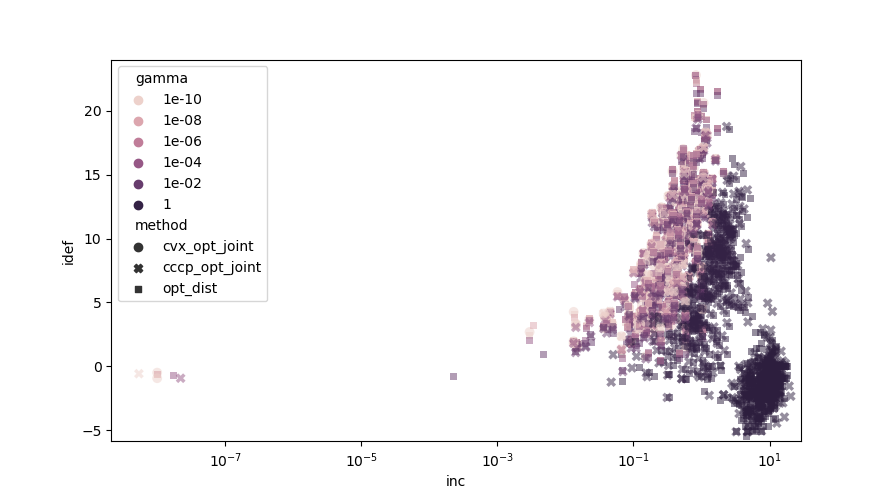
\includegraphics[width=\linewidth]{figs/inc-idef2}
    \caption{An illustration of the trade-off between $\OInc$ and $\SInc_{}$. Darker collors correspond to larger $\gamma$.}\label{fig:inc-idef}
\end{figure}

%joe9
%We now Consider, for example, consider a PDG $\dg M$ containing three
Consider a PDG $\dg M$ containing three
hyperarcs 
$
    \Ar = \{ \ed0XY, \quad \ed{1}{}{X}, \quad \ed2{}Y  \}.
$
% which are associated, respectively, with probabilities $p_1(X), p_2(Y)$, and $p_3(Y|X)$. 
Suppose that the first two contain only structural information, 
while the last contains only observational information. 
Formally, this means that we have $\alpha_1 = \alpha_2 = 1$ while $\alpha_0 = 0$;
and also $\beta_1 = \beta_2 = 0$ (so it doesn't matter what $p_1(X)$ or $p_2(Y)$ are), while $\beta_0 > 0$ and $p_0(Y|X)$ is some conditional distribution on $Y$ given $X$. 

The structure of this PDG asserts that $X$ and $Y$ are independent.
But unless $p_0(Y|X)$ gives the same distribution on $Y$ for every value of $X$, the structural and observational information in this PDG appear to be inconsistent.
This is not quite true, because $X$ might be deterministic, making it independent of $Y$ no matter what. 
In this case, for all $\gamma > 0$ and also in the observational limit, 
$\bbr{\dg M}^*_\gamma$ consists of all disitributions $\mu(X,Y) = \mu(X)p_0(Y|X)$ in which
$p_0(Y|x)$ is identical for all $x$ in the support of $\mu(X)$.

Note that there was no \obslimit\ here, which is possible 
because the condition $\bbeta > 0$ was not met.  Let's tweak the problem slightly, 
and suppose that $\beta_1 > 0$.

Now on the one extreme, we now have an \obslimit\
\[
    \bbr{\dg M}^*_{\epsilon} = p_1(X) p_0(Y|X)
\]
since the observational information alone is enough to determine a unique distribution.
At the other extreme, as $\gamma \to \infty$, the PDG represents those distributions 
in which $\mu(X)$ and $\mu(Y)$ are independent, but come closest to matching.
If, in addition, we assume $\beta_0 = \beta_1$, then we can conclude that
\[
    \bbr{\dg M}^*_{\nf1\epsilon} = p_1(X) p_0(Y) 
\]
where $p_0(Y) := \Ex_{x \sim p_1}[ p_0(Y|x) ]$.
% An illustration of how this can make a difference 
See \cref{fig:inc-idef} for a visual illustration of how this trade-off can happen.
\end{example}


\section{Larger
    \texorpdfstring{$\boldsymbol\gamma$}{Gamma} and the Convex-Concave Procedure (CCCP)}
    \label{sec:larger-gamma}

% Now, suppose we're no longer
Next, let's consider the case where $\gamma$ is
larger, meaning that the structural term $(\SInc_{})$,
becomes more important.
Because 
% $\SInc_{}$
this term can express features of a distribution like indepenedence, it cannot be convex. 
(It is easy to see that the set of distributions that make $X$ and $Y$ is independent is not convex: note that they are independent if either $X$ or $Y$ is deterministic, so if this set were convex, it would include all distributions.)
    % \footnote{one can easily verify that set of distributions that make $X$ and $Y$ independent is not convex.}
Nevertheless, \eqref{eq:altscore} still gives us a way to proceed because it is a decomposition into a sum of a convex and a concave function, meaning that we can apply the convex-concave procedure, or CCCP \parencite{yuille2003concave}.
% The first line is the sum of a linear term and a convex one,
In more detail: and each individual term on the second line is either convex or concave, depending on the sign of the quantity $\gamma \alpha_a - \beta_a$.
Once we sort the terms into convex terms $f(\mu)$ and strictly concave terms $g(\mu)$, we can choose an initial guess $\mu_0$, and iteratively use the convex solver as in \cref{sec:small-gamma} to compute
%
\begin{align*}
    \mu_{t+1} &:= \argmin_{\mu} f(\mu) + (\mu - \mu_{t})^{\sf T}
        \nabla g(\mu_t).
\end{align*}

This can be quite slow becaues each iteration of this algorithm is very expensive, but it is guaranteed to make progress, since
\def\tplus1{{t\mskip-2mu+\mskip-2mu1}}
\begin{align*}
    f(\mu_\tplus1) \!+\! g(\mu_\tplus1) &<  f(\mu_\tplus1) \!+\! (\mu_\tplus1 \!-\! \mu_t)^{\sf T} \nabla g(\mu_t) \!+\! g(\mu_t)
        % &\text{(concavity of $g$)}
        \\
    &\le  f(\mu_t) + (\mu_t - \mu_{t})^{\sf T}\nabla g(\mu_t)  + g(\mu_t)
        % &\text{(defn of argmin)}
    \\
&= f(\mu_t) + g(\mu_t)
\end{align*}
and eventually find an optimum, because the concave terms are bounded (since they are conditional entropies of a finitely supported distribution).
Furthermore, it does better than black-box optimizers when the problem has a concave component.

\subsection{Implementation and Experiments with the CCCP}

In our impementation, one will notice that there is no 
method corresponding to problems \eqref{prob:joint-small-gamma} or \eqref{prob:cluster-small-gamma} --- rather, we have only implemented the CCCP. 
This is because they are special cases of the CCCP, for when the problem happens to satisfy $\bbeta \ge \gamma \balpha$. In this case, the concave part of the function $g$ is identically zero, and one needs precisly one iteration. 


One can see in \cref{fig:gamma-v-gap-fine}, for example, that when $\gamma = 2 > 1 = \max_a {(\beta_a / \alpha_a)}$, 
CCCP performs better than the other methods. One big reason it doesn't do significantly better than it currently does, is because only allow it five iterations, which is already time-consuming.
For combinations of larger $\gamma$ and more worlds, however, this is not nearly enough to converge, while the black-box optimizers are both faster and attain better objective values.

\section{Details on the Empirical Evaluation}\label{sec:expt-setup}
Imagine a very steep $V$-shaped canyon, and inside a small slow-moving stream at a gentle incline. The end of the river may be very far away, and the whole landscape may be smooth and strongly convex, but the gradient will still almost always point perpendicular to it, and rather towards the center of the river.
This intuition may help explain why, even though $\bbr{\dg M}_\gamma$ is infinitely differentiable in $\mu$ and $\gamma$-strongly convex, it can still be challenging to optimize, especially when the $\beta$'s are very different, or when $\gamma$ is small.
For example, a solution to \eqref{prob:cluster-inc} finds a minimizer of $\OInc$, but such minimizers may be very far away from $\bbr{\dg M}_{0^+}^*$, despite sharing an objective value.

We now see how this is true even when working with very small PDGs and joint distributions.

% One interesting feature of this class of problems is that they do not seem to be
% amenable to the same kinds of generic modeling techniques that
%joe4*: this feels like the werong story, but I would need to know
%exactly hwat experiments are performed to know the "right" story.
%oli4: fair enough; this will probably be rewritten. Still, I want to defend the core
% of it. If we could just use gradient descent or other standard black-box optimization
% tools used to train neural networks, at these problems, that would severely undercut
% the story of our paper.  The contrapositive of that is that this is a very expressive
% class of optimization problems (and, I have argued, includes most of probabilistic
% modeling in ML). Not only do those methods have no guarantees, but also it seems they
% do not perform well in practice. This would mean we have found an important class of
% problems on which we can emperically outperform the standard methods!
%joe5: please run a spellchecker.  There are mistakes tha you make
%consistently (like "emperically").  "Empirically" is unrelated to
%"emperors"! 
%oli5: haha it's good to finally know what "emperical" means after using it for all these years! I've replaced the remaining few of these and will run a complete spell check in the next iteration. 

\begin{figure}
    % 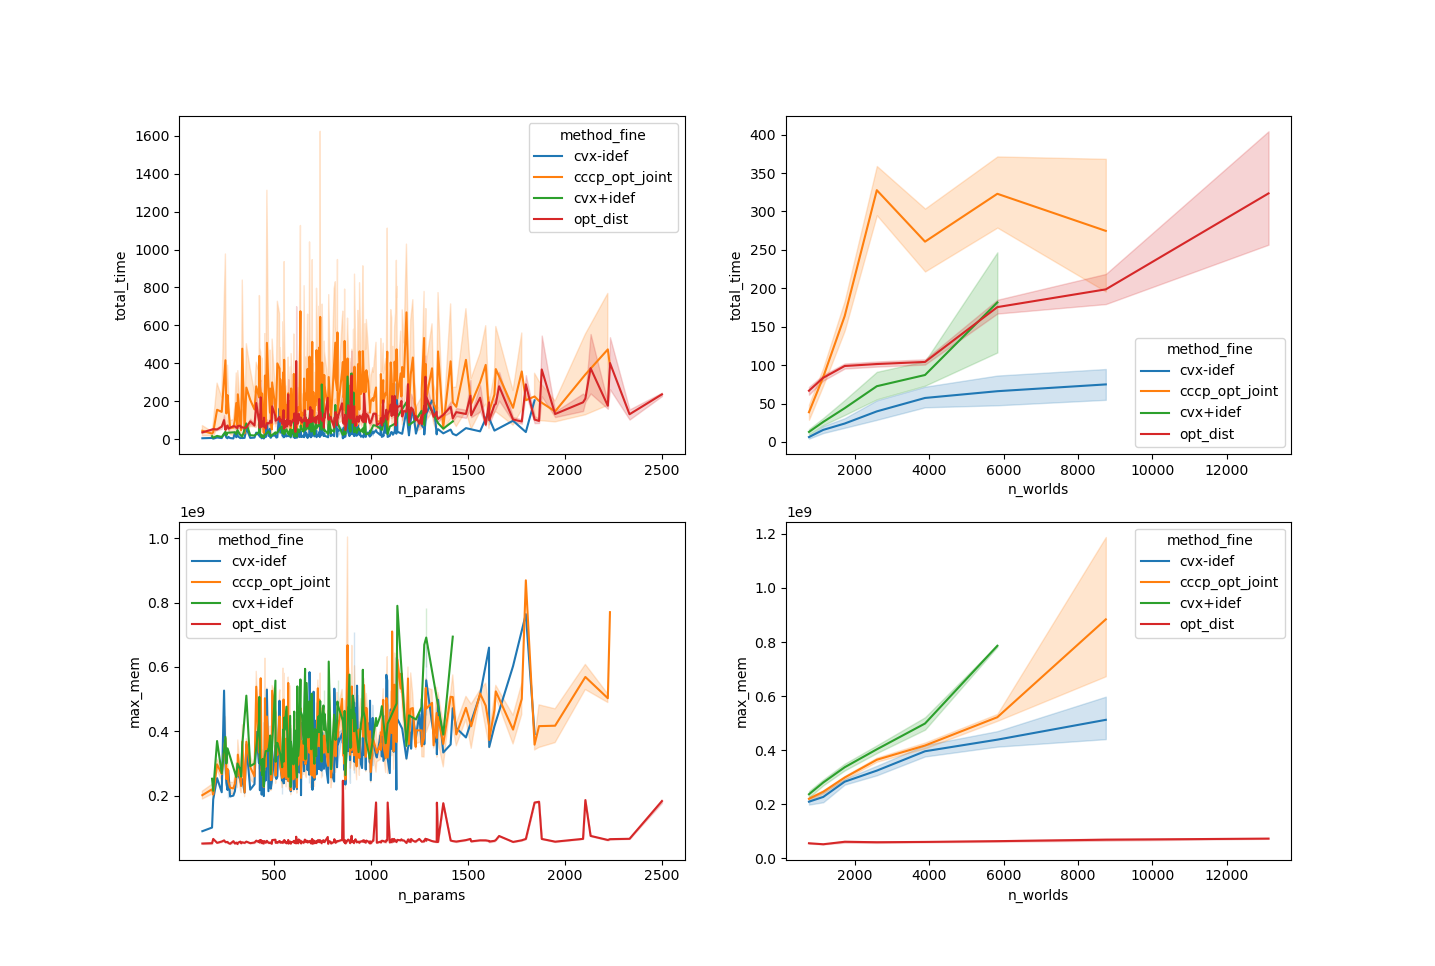
\includegraphics[width=\linewidth]{figs/resources-fine}
    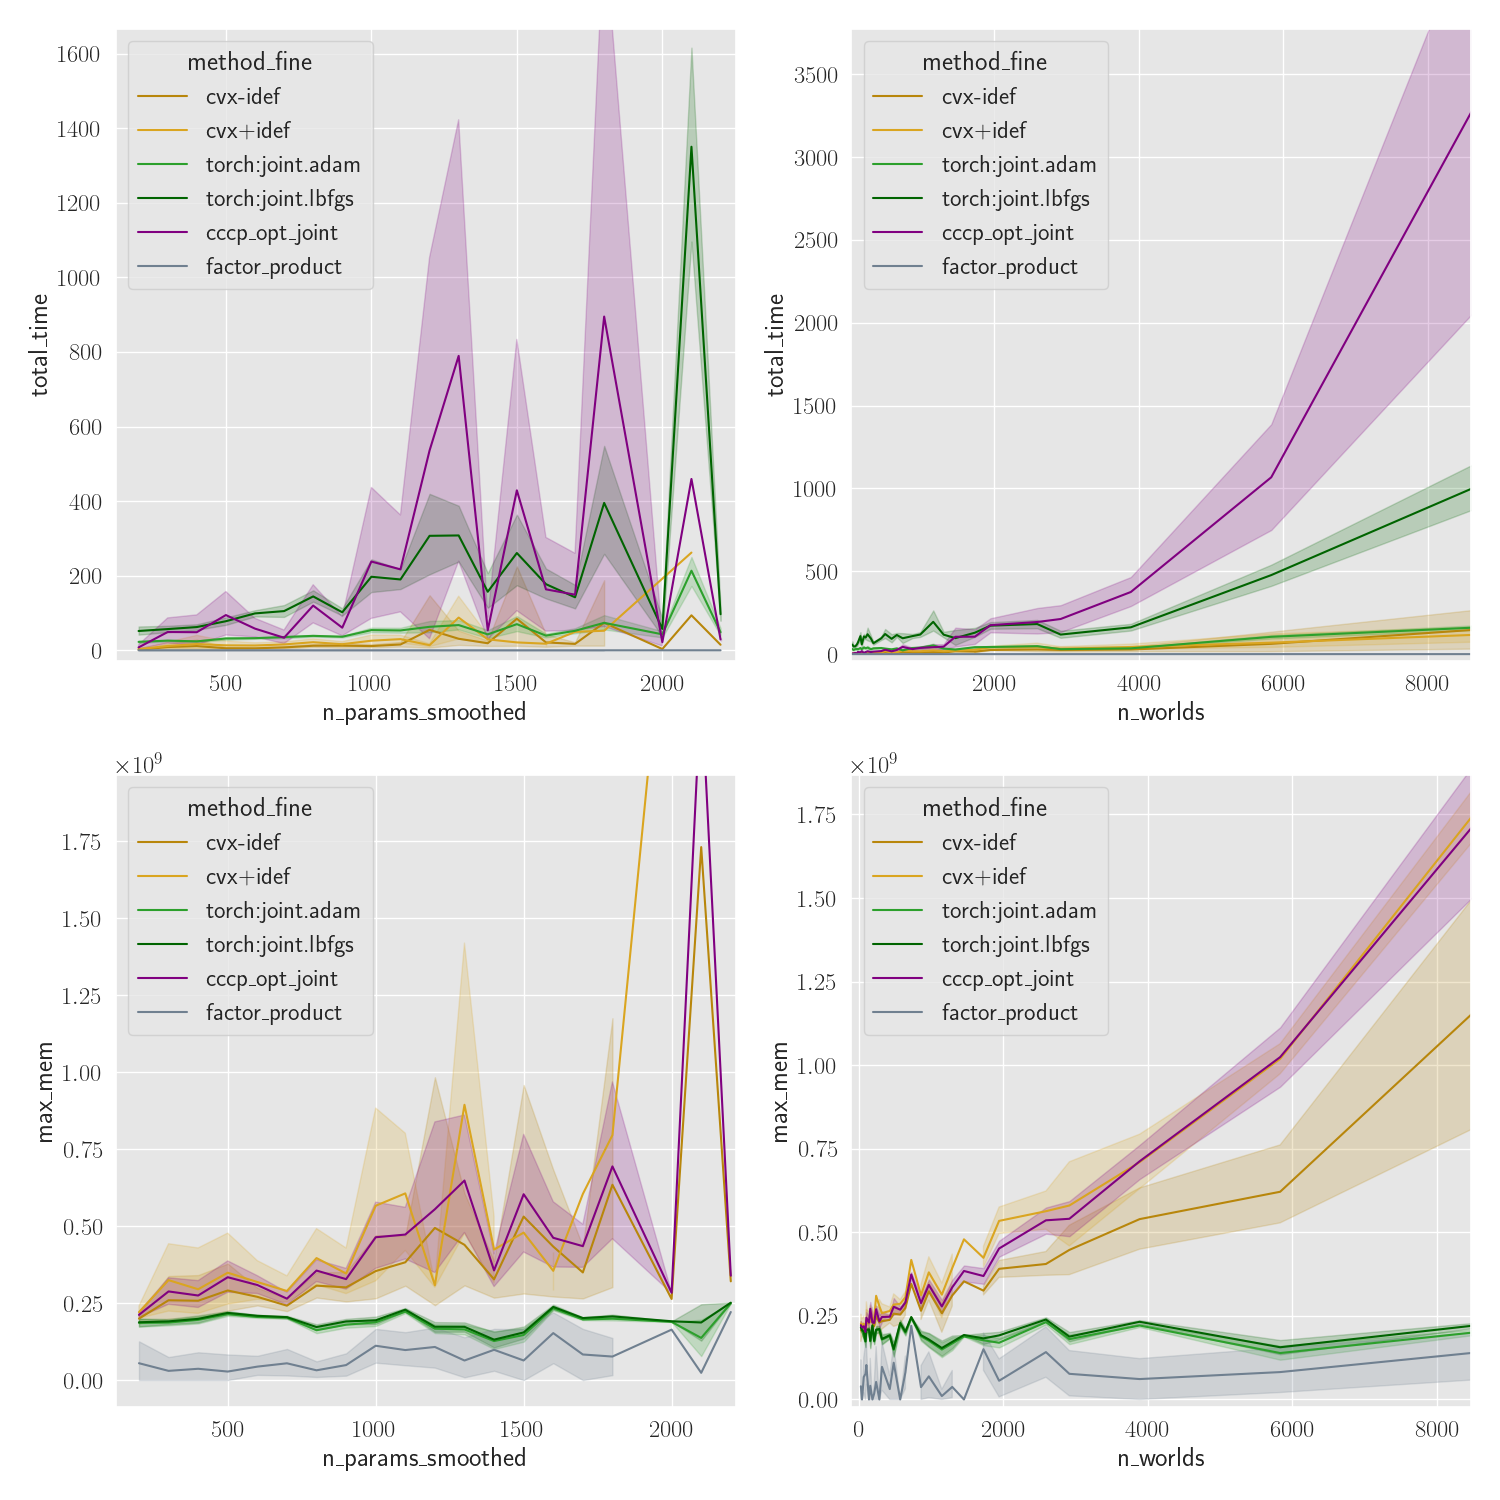
\includegraphics[width=\linewidth]{figs/rand-joint/resource-costs}
    \caption{\small
        Resource costs for the joint-distribution optimization setting of \cref{sec:inf-as-cvx-program}.
        We measure computation time (\texttt{total\_time}, top) and maximum memory usage (\texttt{max\_mem}, bottom) for the various optimization methods (by color), as the size of the PDG increases, as measured by the number of parameters in the PDG (\texttt{n\_params}$\,=\V\!\Ar$, left), and the size of a joint distribution over its variables (\texttt{n\_worlds}$\,=\V\!\X$, right).
        Note that the convex solvers for the 0 and $0^+$ semantics are significantly faster than LBFGS, and on par with Adam.
        % However, the small-$\gamma$ method (\verb|cccp_opt_joint|)
        However, all three convex-solver based approaches require significantly more memory than the black-box optimizers.
     }\label{fig:resources}
\end{figure}



% \textbf{Comparison to Black-Box Optimizers, on Joint Distributions. }
\subsection{Synthetic Experiment: Comparison with Black-Box Optimizers, on Joint Distributions.} \label{sec:joint-expt-details}
% Even without the fancier construction 
% From an optimization perspective, 
% one interesting feature of PDG inference
% is that, despite having incredibly nice properties
% We begin with some results on joint distributions; 
% the experimental setup is described in \cref{sec:expt-setup}.
 % applying black-box optimization methods such as gradient descent and LBFGS, do not seem to reliably find minima of \eqref{eqn:scoring-fn}.
% \textit{Resources.}
\begin{wrapfigure}{R}{4.8cm}
    \centering
    \vspace{-3ex}
    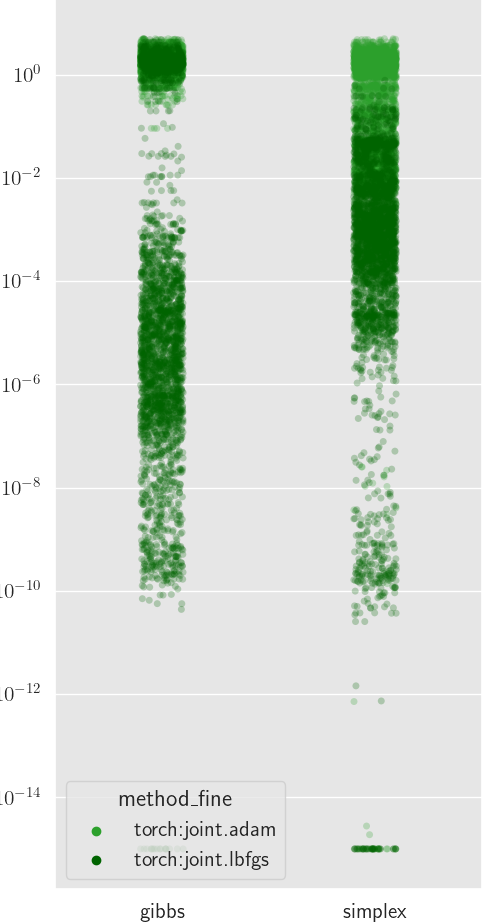
\includegraphics[width=4.5cm]{figs/rand-joint/representation}
    \caption{\small differences in performance between the Gibbs and simplex parameterizations of probabilities.}%
    \label{fig:representation}%
\end{wrapfigure}


Here is a more precise description of our first synthetic experiment,
on joint distributions, which contrasts the convex optimization approaches of \cref{sec:inf-as-cvx-program} with black-box optimizers.



\begin{itemize}
    \item generate 300 PDGs, each of which has the following quantities, to each of which we choose the following natural numbers uniformly at random:
    \begin{itemize}
        % [nosep,label={$\blacktriangleright$}]
        \item the number $N \in \{5,\ldots,9\}$ of variables
            (so that $\X := \{1, \ldots, N\}$),
        \item the number $V_X \in \{2, 3\}$ values per variable
            (so that $|\V X| = V_X$ for each $X \in \X$)
        \item the number $A \in \{7, \ldots, 14\}$ hyperarcs,
        each $a \in \{1, \ldots, A\} =: \Ar$ of which has
        \item $N^S_a \in \{0, 1, 2, 3\}$ sources, and
        \item $N^T_a \in \{1,2\}$ targets.
    \end{itemize}
    \item For each arc $a \in \Ar$, $N^S_a$ of the $N$ variables are choosen without replacement to be sources $S_a \subseteq N$, and $N^T_a$ of remaining variables are chosen to be targets. Finally, to each value of $S_a$ and $T_a$, a number $p_{a,s,t} \in [0,1]$ is chosen uniformly at random, and the cpd 
    \[
     \p_a(\Tgt a {=} t \mid \Src a {=} s) = \frac{p_{a,s,t}}{\sum_{t' \in \V(T)} p_{a,s,t'}}
     \qquad\text{ is given by normalizing appropriately.}
    \]
    This defines a PDG $\dg M = (\X, \Ar, \mathbb P, \mat 1, \mat 1)$, that
    has $\balpha = \bbeta = \mat 1$, which will allow us to comapre against
    belief propogation and other graphical models at $\gamma = 1$.
    The complexity of this PDG is summarized by two numbers:
    \begin{itemize}[nosep]
        % \item \texttt{n\_edges}, the number of edges in $\dg M$,
        \item \texttt{n\_params}$\,:= \V\!\Ar$, the total number of parameters in all cpds of $\dg M$, and
        \item \texttt{n\_worlds}$\,:= \V\!\X$, the dimension of joint distributions over $\dg M$'s variables.
    \end{itemize}
\end{itemize}

\begin{itemize}    
    \item Run MOSEK on \eqref{prob:joint-inc} to find a distribution that minimizes $\OInc$; we refer to this method as \texttt{cvx-idef}
    \item Use the result to run MOSEK on \eqref{prob:joint+idef} to
      find the special distribution $\bbr{\dg M}^*_{0^+}$; we refer to
%joe9*: Why not just call it cvxsinc and cut the remaining sentences?
      this method as \texttt{cvx+idef}. These names are due to the
      fact that $\SInc$ is called $\IDef{}$ in previous work
      \parencite{pdg-aaai,one-true-loss}; 
    thus, this refers to using the convex solver to compute minimizers of $\OInc$ with and without considering $\IDef{}$.
    
    \item Now for the torch baselines. 
    Let $\theta = [\theta_{\mat x}]_{\mat x \in \V\X} \in \mathbb R^{\V\X}$, be a vector of optimization variables, and choose a representation of the joint distribution, either by
    \[
    % $\displaystyle
        \Big(\begin{array}{c}\text{renormalized}\\
        \text{simplex}\end{array}\Big)\quad
        \mu_{\theta}(\mat x) = \frac{\max\{\theta_{\mat x}, 0\} }
            {\sum_{\mat y \in \V\!\X}\max\{\theta_{\mat y}, 0\} }
    % $.
    \qquad\text{or}\qquad
    \mu_{\theta}(\mat x) = \frac{\exp(\theta_{\mat x})}{\sum_{\mat y \in \V\!\X} \exp(\theta_{\mat y})}\quad(\text{Gibbs})
    \qquad\quad\text{(see \cref{fig:representation})}
    \]
    \item 
    Then, for each value of gamma: $\gamma \in \{0, 10^{-8}, 10^{-4}, 10^{-2}, 1\}$, and each learning rate $\texttt{lr} \in 1E-3, 1E-2, 1E-1, 1E0$, and each optimizer $\mathit{opt} \in \{\texttt{adam}, \texttt{L-BFGS}\}$, 
    run $\mathit{opt}$ over the parameters $\theta$ to minimize $\bbr{\dg M}_\gamma(\mu_{\theta})$
     until convergence (or a maximum of 1500 iterations)  
     
     \item We collect the following data about the resulting distribution and the process of computing it:
     \begin{itemize}[nosep]
         \item the total time taken to arrive at $\mu$;
         \item the maximmum memory taken by the process computing $\mu$;
         \item the objective and its component values:
         \vspace{-1ex}
         \[
            \texttt{inc} := \SInc_{\dg M}(\mu),
            \qquad \texttt{idef} := \SInc_{\dg M}(\mu),
            \qquad \texttt{obj} := \OInc_{\dg M}(\mu) + \gamma \SInc_{\dg M}(\mu) = \bbr{\dg M}_\gamma(\mu) 
        \]
     \end{itemize}
\end{itemize}



The numbers can then be recreated by running our experimental script as follows:
\begin{verbatim}
python random_expts.py -N 300 -n 5 9 -e 7 14 -v 2 3
    --ozrs lbfgs adam
    --learning-rates 1E0 1E-1 1E-2 1E-3
    --gammas 0 1E-8 1E-4 1E-2 1E0
    --num-cores 20
    --data-dir random-joint-data
\end{verbatim}
which creates a folder called \verb|random-joint-data|,
and fills it with \verb|.mpt| files corresponding to each distribution
and the method / parameters that gave rise to it. 

\textbf{Analyzing the Results.}
Look at  \cref{fig:resources}.  Our theoretical analysis, and in particular the proof of \cref{lem:cluster-inc-polytime}, suggest that the magnitudes of $\V\!\X$ and $\V\!\Ar$ play similar roles in the asymptotic complexity of PDG inference. 
Our experiments reveal that, at least for random PDGs, the number of worlds is the far more important of the two; observe how much more variation there is on the left side of the figure than the right---and now note that the left side has been smoothed, while the right side has not.
% Observe also that the time complexity of L-BFGS seemst to be growing at a larger rate than 
The black-box py-torch based approaches clearly have an edge in that they can handle larger models, as evidenced by the cut-offs on the right-hand side of \cref{fig:gap-resource-fine-old}, when with 5GB memory.

Note that the exponential-cone-based methods for the observational limit (gold) are actually faster than L-BFGS (the black-box optimizer with the lowest gap), and also seem to be growing at a slower rate.
However, they use significantly more memory, and cannot handle large models.
In addition to being faster, our techniques also seem to be more precise; they achieve objective values that are consistently much better than the black-box methods.
% Recall 


Now look at \cref{fig:joint-gap-vs-time-by-gamma},
which contains a break-down of the information in \cref{fig:joint-gap-time}. The bottom half of the figure is just the same information, but with each value of $\gamma$ separated out, so that the special cases of the factor product and $0^+$ inference become clear, while the top half shows why it's more important to look at the gap than the actual objective value for these random PDGs. 
\Cref{fig:joint-gap-vs-time-by-gamma} also makes it clearer how larger problems take longer, and especially so for \texttt{cccp} (violet), which solves the most complex version of the problem \eqref{prob:joint-small-gamma}.

\begin{figure}
    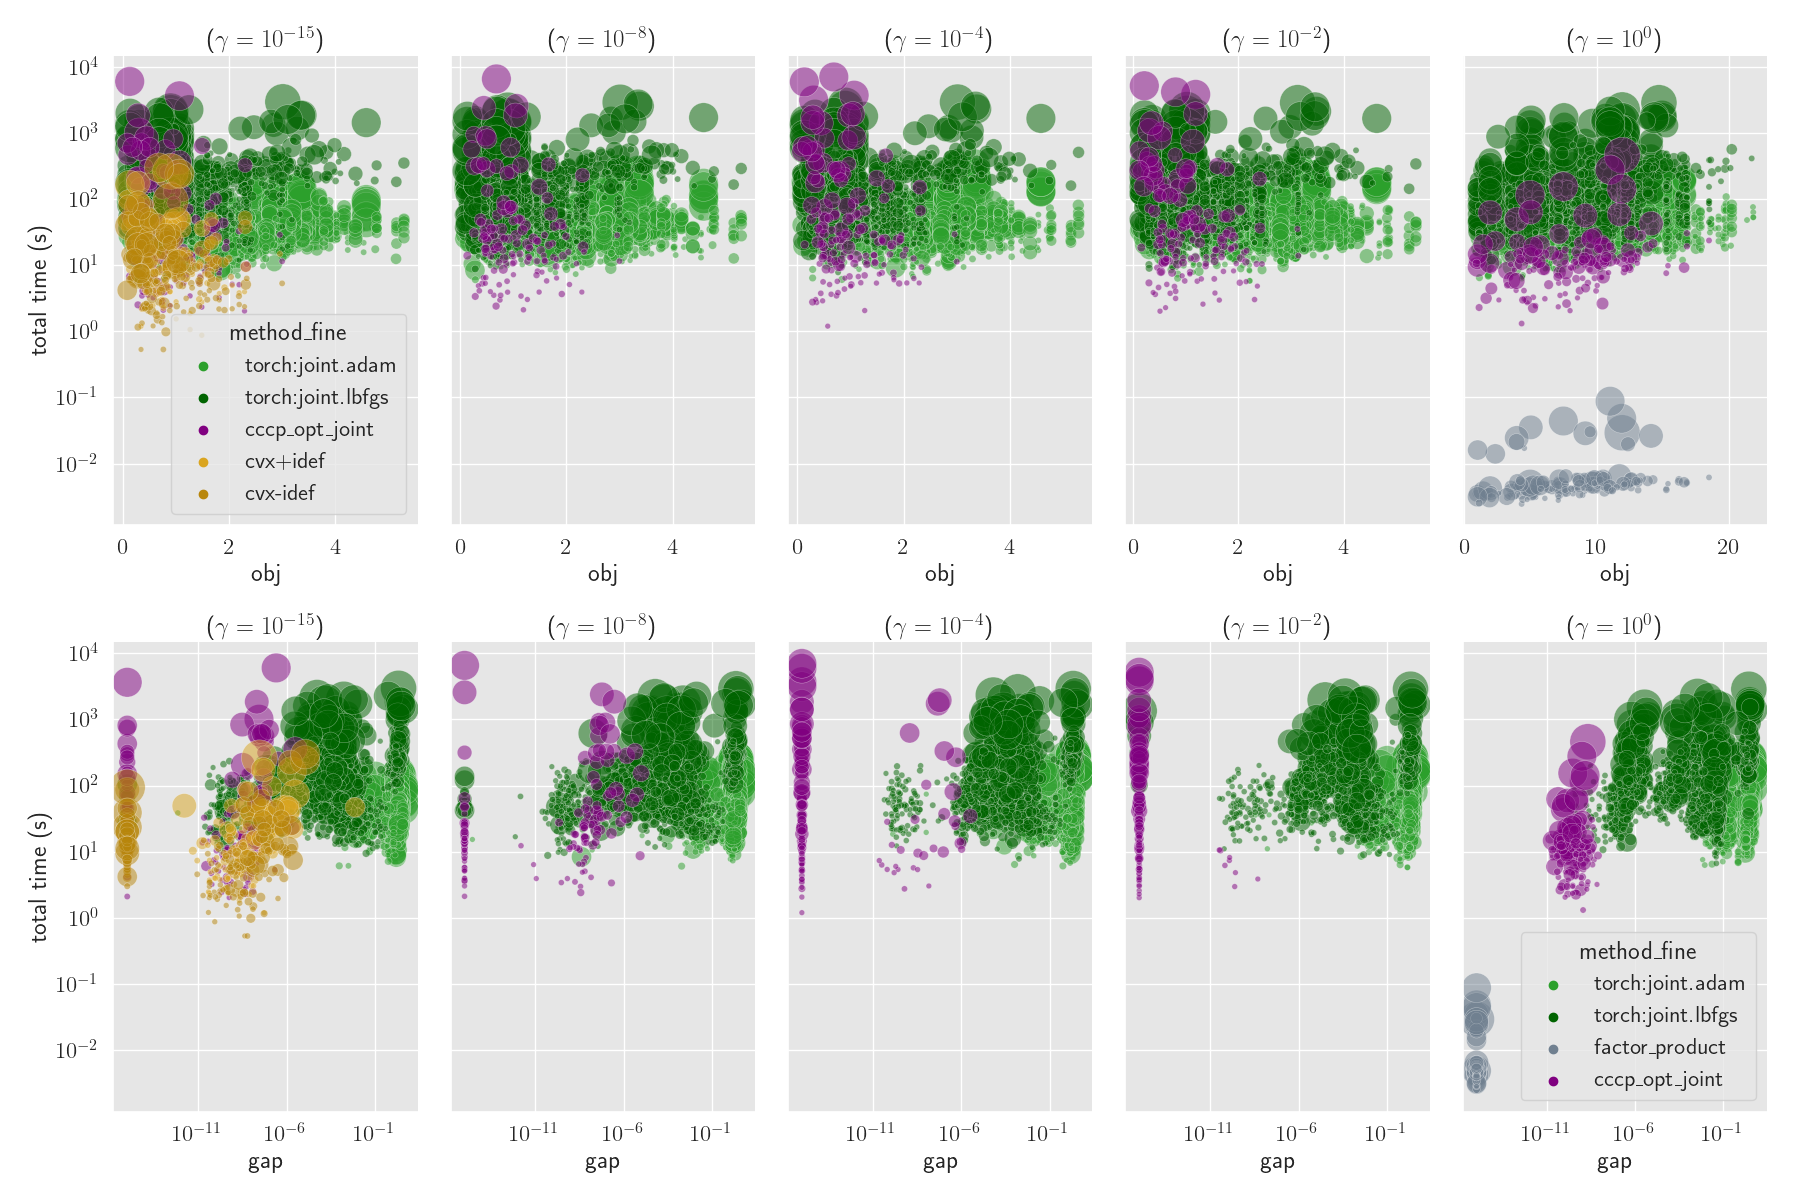
\includegraphics[height=0.45\textheight]{figs/rand-joint/gap-vs-time-by-gamma}
    \caption{\small
        An un-compressed version of the information in \cref{fig:joint-gap-time}, that groups by the value of $\gamma$, and also gives the absolute values of the objectives (top row) in addition to the relative gaps (bottom row).
    }\label{fig:joint-gap-vs-time-by-gamma}
\end{figure}




\discard{\begin{figure}
    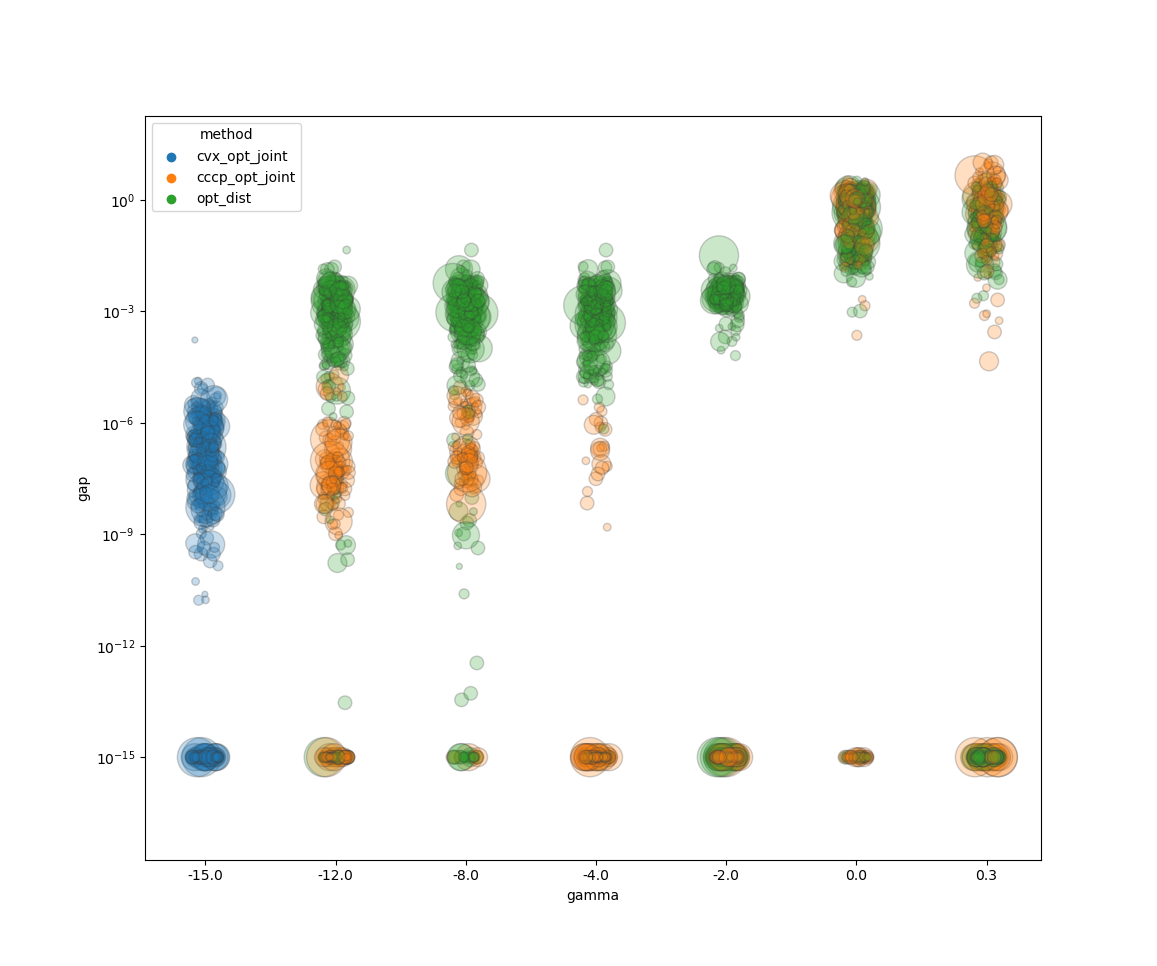
\includegraphics[height=0.45\textheight]{figs/gamma-vs-gap-bettergap}
    \caption{
        A graph of the gap (the difference between the attained objective value, and the best objective value obtained across all methods for that value of $\gamma$),
        as $\gamma$ varies. The x-axis is $\log_{10} ( \gamma + 10^{-15})$.
        As before, colors indicate the optimization method; here blue corresponds to \eqref{prob:joint+idef}, while orange corresonds to \eqref{prob:joint-small-gamma}, and green, as before, correponds to all optimization baselines.
        The size of the circle illustrates the relative number of worlds.
        See \cref{fig:gamma-v-gap-fine} for a more detailed breakdown.
    }\label{fig:gamma-v-gap}
\end{figure}}


\begin{figure}
    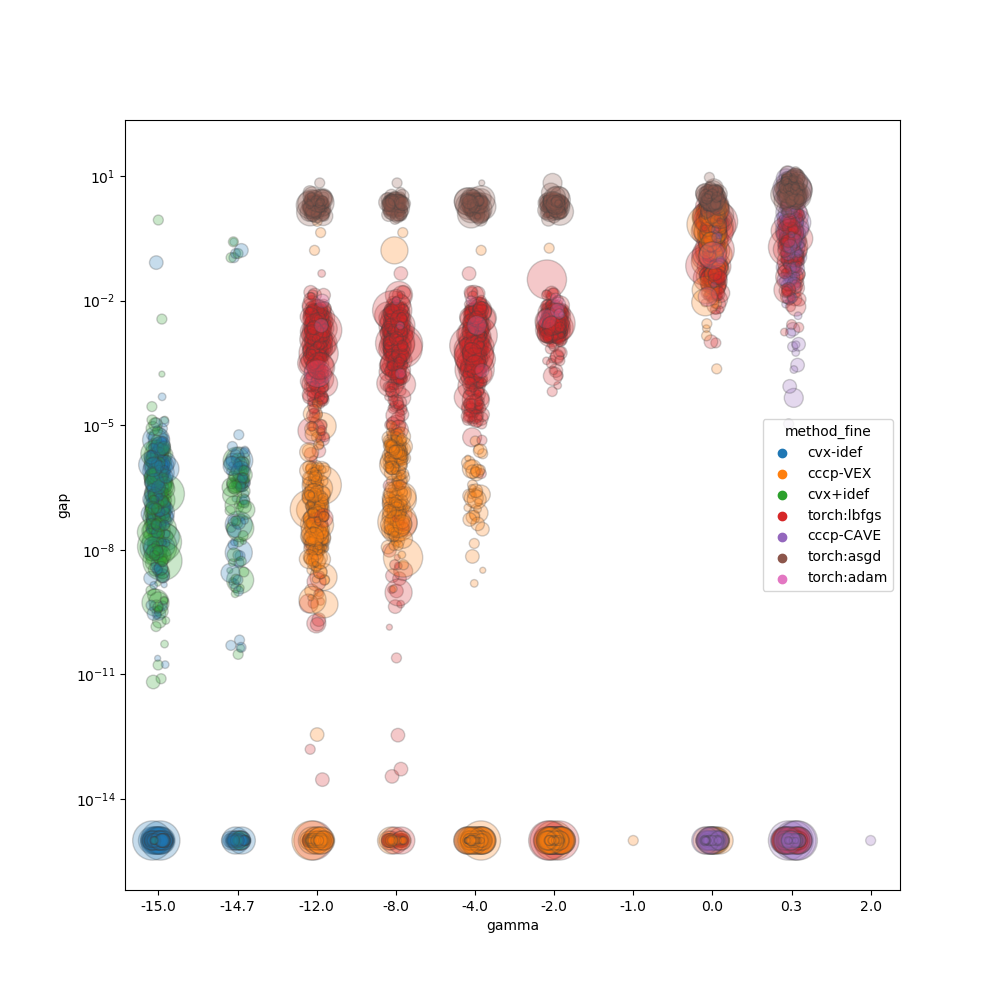
\includegraphics[width=\linewidth]{figs/2}
    \caption{
        A graph of the gap (the difference between the attained objective value, and the best objective value obtained across all methods for that value of $\gamma$),
        as $\gamma$ varies. The x-axis is $\log_{10} ( \gamma + 10^{-15})$.
        As before, colors indicate the optimization method, and
        the size of the circle illustrates the number of optimization variables (i.e., the number of possible worlds).
        % A fine-grained variant of \cref{fig:gamma-v-gap}, which splits each method into sub-groups.
        \texttt{cvx-idef} corresponds to just solving \eqref{prob:joint-inc}, and \texttt{cvx+idef} corresponds to then solving problem \eqref{prob:joint+idef} afterwards.
         % depending on whether or not it also computed the second step described in \cref{sec:empirical-limit} to account for $\SInc_{}$.
        The CCCP runs are split into regimes where the entire problem is convex ($\gamma \le 1$, \texttt{cccp-VEX}), and the entire problem is concave ($\gamma > 1$, \texttt{cccp-CAVE}).
        The optimization approaches \texttt{opt\_dist} are split into three different optimizers: LBFGS, Adam, and also a third one that is relatively poor: accelerated gradient descent.
        Note that for small $\gamma$, the exponential-cone based methods significantly outperform the gradient-based ones.
    }\label{fig:gamma-v-gap-fine}
\end{figure}


%joe9
%\subsection{Synthetic Experiment: Comparing with Black-Box Optimizers,
\subsection{Synthetic Experiment: Comparing with Black-Box Optimizers
  on Clique Trees} \label{sec:clus-expt-details} 

\begin{figure}
    \centering
    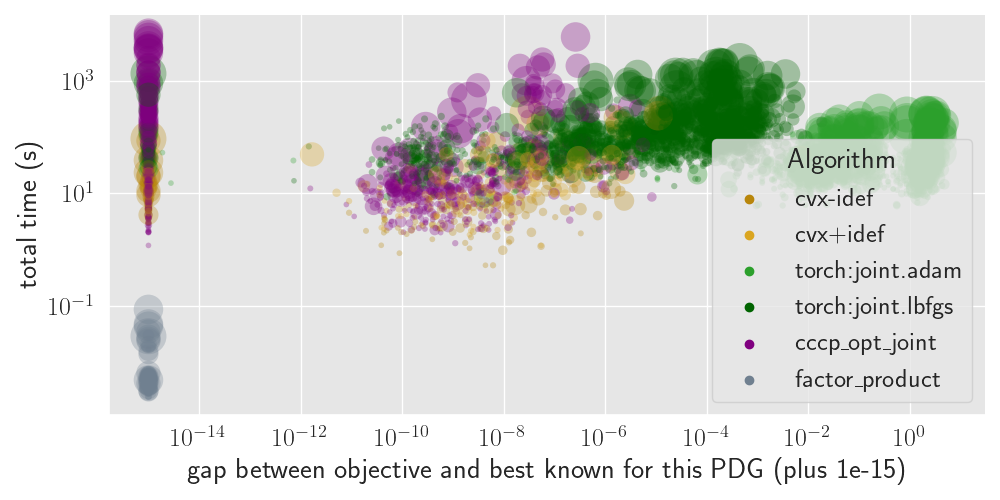
\includegraphics[width=0.67\linewidth]{figs/rand-clus/gap-vs-time}
    \caption{An analogue of \cref{fig:joint-gap-time}, for the cluster setting.
    Note that there is even more separation between the exponential-cone based approaches, and the black-box optimization based ones.
    The new grey points on the bottom correspond to belief propogation, which is both faster and typically the most accurate.}
    \label{fig:clus-gap-vs-time}
\end{figure}
\begin{figure}
    \centering
    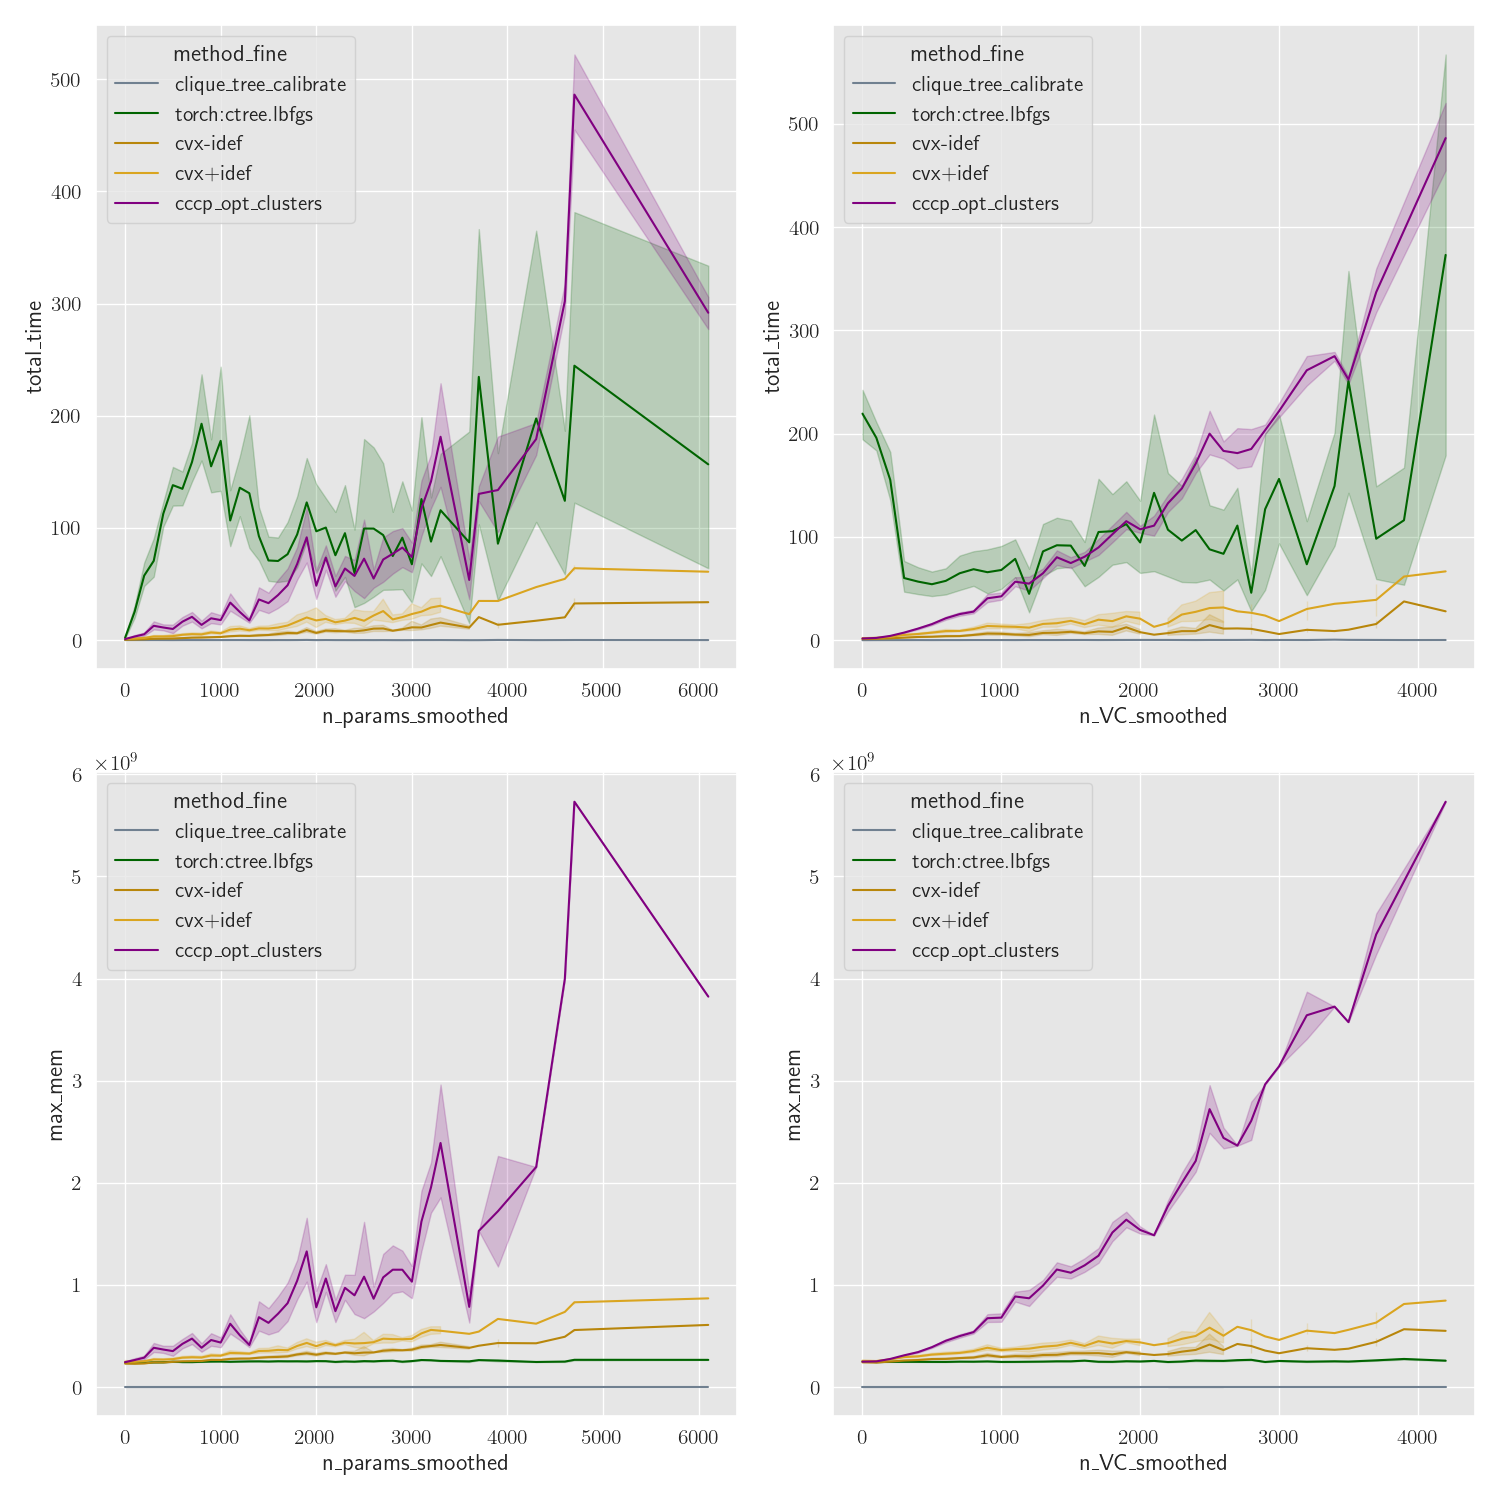
\includegraphics[width=0.67\linewidth]{figs/rand-clus/resource-costs}
    \caption{Resource costs for the cluster setting. Once again, the $\OInc$-optimimzing exponential cone methods are in gold, the small-gamma and CCCP is in violet, and the baselines are in green. The bottom line is belief propogation, which is significantly faster and requires very little memory, but also only gives the correct answer under very specific cirucumstances.}
    \label{fig:clus-resource-costs}
\end{figure}

%joe9*: You need a little glue here to give the reader the big picture.

\begin{enumerate}
    \item Choose a number of variables $N \in \{ 8, \ldots, 32 \}$, and a treewidth $k \in \{1, \ldots, 4\}$ uniformly at random. 
    Then, draw a random $k$-tree and corresponding tree of clusters $(\C, \mathcal T)$, as follows:
    \begin{enumerate}
        \item initialize $G \gets K_{k+1}$ to a complete graph on $k+1$ vertices, and $\C \gets\{ K_{k+1} \}$ to be set containing a single cluster, and $\mathcal T\gets \emptyset$.
        \item until there are $N$ vertices: add a new vertex $v$ to $G$, then randomly select a size $k$-clique (fully-connected subgraph) $U \subset G$, and add edges between $v$ and every vertex $u \in U$.
        Then, add $U \cup \{v\}$ to $\C$, and add edges to every other cluster $C \in \C$ such that $U \subset C$.
    \end{enumerate}
    % It is well-known that this procedure gives a tree; see, for instance,
    % \cite{}
    \item Then, draw the same parameters $V_X \in \{2,3\}$, $A \in \{8, \cdots, 120\}$, $N_a^S \in \{0,1,2,3\}$, and $N^{T}\in \{1,2\}$ 
    as in \cref{sec:joint-expt-details} uniformly at random.
    While $N_a^S + N^T_a > k+1$, for any $a$, resample $N_a^S$ and $N_a^T$.
    
    \item Form a PDG whose structure $\Ar$ can be decomposed by $(\C, \cal T)$, as follows: 
    for each edge $a \in \Ar$, sample a cluster $C \in \C$ uniformly at random; then select $N_a^S$ nodes from that cluster without replacement as sources, and $N_a^T$ nodes as targets; this is possible because each cluster has $k+1$ nodes, and $N_a^S + N_a^T \le k+1$ by construction.
    \item Fill in the probabilities by drawing uniform random numbers and re-normalizing, just as before, to form a PDG $\dg M$
    
    \item The black-box optimization baselines work in much the same way also, although now the optimization variables include not one distribution $\mu$ but a collection $\bmu$ of them; 
    this time, we use only the simplex representation of $\bmu_\theta$.
    More importantly, we want these clusters to share appropriate marginals; to encourage this, we add a terms to the loss function, so overall, it is
    \[
        \ell(\theta) := \bbr{\dg M}_{\gamma}(\bmu_{\theta}) + \sum_{C{-}D \in \mathcal T} \exp \left(\sum_{w \in \V(C\cap D)} \Big(\mu_C(C\cap D{=}w) - \mu_D(C \cap D {=}w)\Big)^2 \right) - 1.
    \]
    This is admittedly pretty ad-hoc; the point is just that it is zero and does not contribute to the gradient if $\bmu_\theta$ is calibrated, and otherwise quickly becomes overwhelmingly important.
    % \begin{enumerate}
    %     \item 
    % \end{enumerate}
\end{enumerate}

\textbf{Analyzing the Results.}
Observe in \cref{fig:clus-gap-vs-time} that the separation between the clique tree convex solver and the black-box algorithms is even more distinct. This is because, in this case, the penalty for violating constraints was too small, and the optimization effort was largely wiped out by the calibration before evalution. 


\begin{figure}
    \centering
    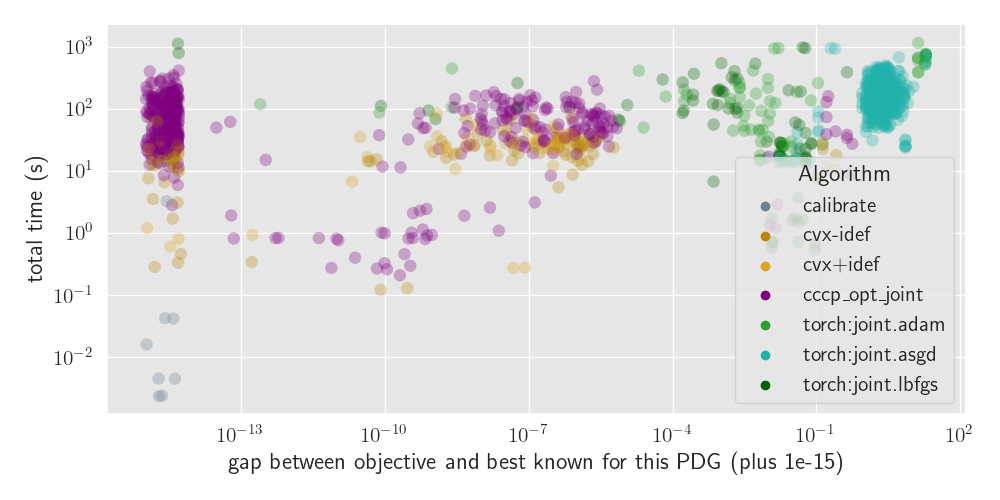
\includegraphics[width=0.7\textwidth]{figs/bn/gap-v-time}
    \caption{Gap vs inference time for the small PDGs in the \href{https://www.bnlearn.com/bnrepository/}{\texttt{bnlearn}} repository}
    \label{fig:bn-gap-v-time}
\end{figure}

This illustrates another general advantage that the convex solver has over black-box optimizers: it is much less brittle and reliant and exactly tuning parameters correctly. Note that even in this minimal example, there were many hyper-parameters that require tuning:
the regularization strengths that enforce soft constraints (clique tree calibration, normalization), as well as learning rate, not to mention
various other structural choices: the optimizer, the representation of the distribution, and the maximum number of iterations, none of which are clear-cut choices, but rather require first being tuned to the data.
While the convex solver does have internal parameters (tolerences and such) these do not need to be tuned to the problem under normal circumstances.

%joe9
%\subsection{Comparing to Belief Propagation, on Clique Trees.}
\subsection{Comparing to Belief Propagation on Clique Trees.}
    \label{sec:bn-expt-details}
 Since PDGs generalize other graphical models, one might wonder how
 our method stacks up against algorithms tailored to the more
%joe9: don't undercut your own paper!
% traditional models. In brief: our algorithm is much slower, and only
 % handle much smaller networks.
  traditional models. In brief: our algorithm is slower, and 
 handles only smaller networks.  
 Concretely, our methods can handle all of the ``small'' networks, and some of the ``medium'' ones, from the \href{https://www.bnlearn.com/bnrepository/}{\texttt{bnlearn}} repository. 
  In these cases, we have verified that the two methods yield the same results.
  \Cref{fig:bn-gap-v-time} contains the analogue of \cref{fig:joint-gap-time,fig:clus-gap-vs-time}
  for the Bayesian Nets. This graph looks qualitatively quite similar to the other graphs we've seen, suggesting that the results in our synthetic experiments hold more broadly for small real-world models as well.
  

  

 \begin{figure}
     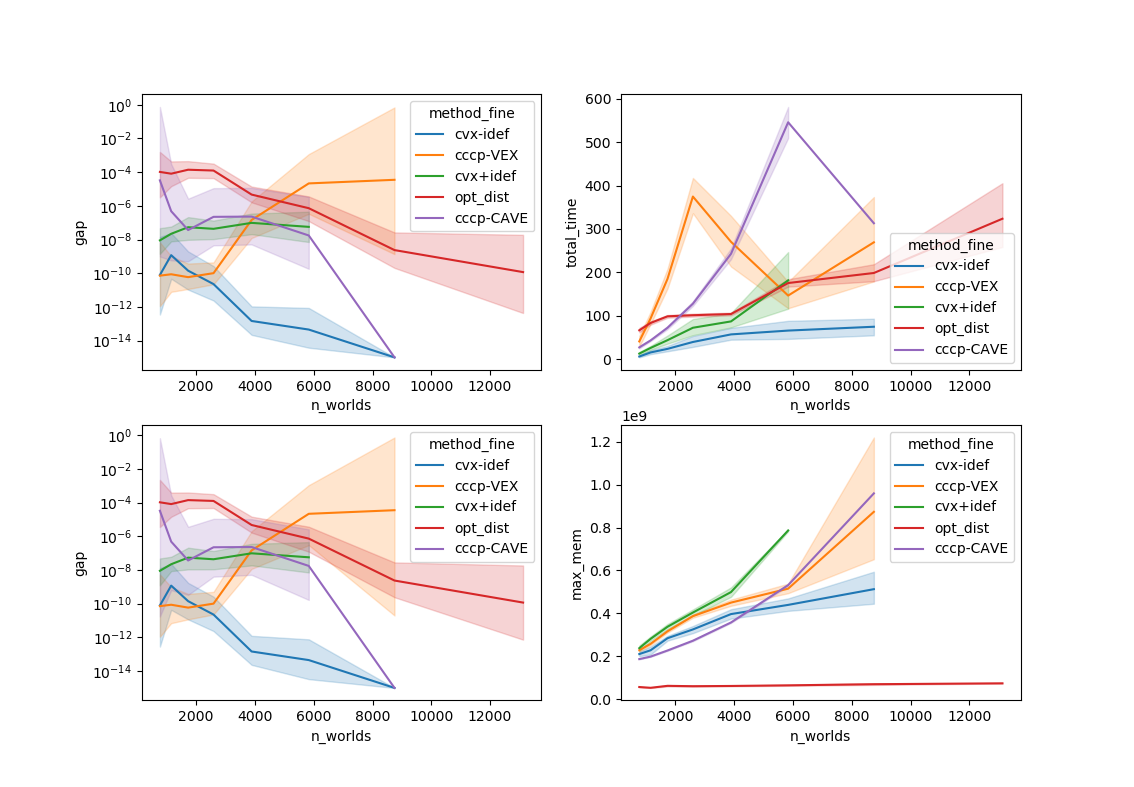
\includegraphics[height=0.45\textheight]{figs/1}
     \caption{
         A variant of \cref{fig:resources}, with 
         with gap (accuracy) information on the left, and slightly different parameter settings. 
     }\label{fig:gap-resource-fine-old}
 \end{figure}


%joe9: it seems silly to have an appendix to an appendix
 \section{Further Proofs, for Appendix Material}

\recall{prop:smooth-and-strictly-cvx}
\begin{lproof}\label{proof:smooth-and-strictly-cvx}
	% First, we deal with the convexity, for which we make use of \cref{lem:cvx2}.
	% \commentout{
	% 	\def\mw#1{{\mat w}_{\!_{#1}}}
	% 	\def\ofmw(#1|#2){(\mw{#1} | \mw{#2})}
	% 	\begin{align*}
	% 		\aar{\dg M \bundle p}_\gamma &= \inf_\mu \Big[ \OInc_{\dg M \bundle p}(\mu)
	% 			+ \SInc_{\dg M \bundle p}(\mu) \Big] \\
	% 		&=  \inf_{\mu} \Ex_{\mat w \sim \mu}
	% 			\left[\log \mu(\mat w) +
	% 			 	\beta_p \log \frac{\mu\ofmw(Y|X)}{p\ofmw(Y|X)} \; +  \!\sum_{\ed LAB} \beta_L \log \frac{\mu\ofmw(B|A)}{\bp\ofmw(B|A)} + \alpha_L \log \frac{0}{\mu\ofmw(B|A)}\right] \\
	% 		&= f
	% 	\end{align*}
	% }
	We start by expanding the definitions, obtaining
	\begin{align*}
		\aar{\dg M \bundle p}_\gamma &= \inf_\mu ~\bbr{\dg M \bundle p}_\gamma(\mu) \\
			&= \inf_\mu \left[ \bbr{\dg M }_\gamma(\mu)
				+ \Ex_{x\sim\mu_{\!_X}} \kldiv[\Big]{\mu(Y\mid x)}{p(Y\mid x)} \right]\\
			&= \inf_\mu \left[ \bbr{\dg M }_\gamma(\mu)
				+  \kldiv[\Big]{\mu(X,Y)}{p(Y \mid X)\, \mu(X)} \right].
	\end{align*}
	% % Choose $\gamma < \min (\{1\}\cup\{ \beta^{\dg M}_L : L \in \Ed^{\dg M}\})$.
	% Since $\bbr{\dg M}_\gamma$ is a $\gamma$-strongly convex function of $\mu$ for all
	% such $\gamma < \min_L \beta_L$, and
	% $\kldiv{\mu_{XY}}{\mu_X \; p_{Y\mid X}}$ is 1-strongly
	% convex in $p$ for fixed $\mu$ (\cref{lem:Dstrongcvx}),
	% % $\thickD$ is convex in both of its arguments,
	% their sum is $\gamma$-strongly convex in $\mu$ and in $p$.
	% By \cref{lem:cvx2} taking an infemum preserves this convexity,
	% and so
	% $
	%  	\inf_\mu \left[ \bbr{\dg M }_\gamma(\mu)
	% 	+  \kldiv[\big]{\mu_{XY}}{p_{Y \mid X}\; \mu_X} \right]
	% $, which equals $\aar{\dg M \bundle p}_\gamma$,
	% is $\gamma$-strongly convex in $p$.
	% % $\aar{\dg M \bundle p}_\gamma$ is smooth
	% % Smoothness.


	% Choose $\gamma < \min (\{1\}\cup\{ \beta^{\dg M}_L : L \in \Ed^{\dg M}\})$.
	Fix $\gamma < \min_L \beta_L$. Then we know that $\bbr{\dg X}_\gamma(\mu)$ is a $\gamma$-strongly convex function for every PDG $\dg X$, and hence there is a unique joint distribution which minimizes it.

	\textbf{Strict Convexity.}
	Suppose $p_1(Y \mid X)$ and $p_2(Y\mid X)$ are two cpds on $Y$ given $X$.
	Fix $\lambda \in [0,1]$, and set $p_\lambda = (1-\lambda) p_1 + \lambda p_2$.
	Let $\mu_1, \mu_2$ and $\mu_\lambda$ be the joint distributions that minimze $\bbr{\dg M \bundle p_1}_\gamma$, $\bbr{\dg M \bundle p_2}_\gamma$ and $\bbr{\dg M \bundle p_\lambda}_\gamma$, respectively.  Then we have
	\begin{equation*}
		\aar{\dg M \bundle p_\lambda}_\gamma
			= \bbr{\dg M}_\gamma(\mu_\lambda) + \kldiv[\Big]{\mu_\lambda(X,Y)}{p_\lambda(Y\mid X) \mu_\lambda( X)}.
	\end{equation*}
	By convexity of $\bbr{\dg M}$ and $\thickD$, we have
	\begin{align}
		\bbr{\dg M}_\gamma(\mu_\lambda)
		 	&\le (\lambda-1)\bbr{\dg M}_\gamma(\mu_1) + \lambda \bbr{\dg M}_\gamma(\mu_2)
			 	\label{eqn:score-cvx}\\
		\text{and}\qquad \kldiv[\Big]{\mu_\lambda(XY)}{p_\lambda(Y | X) \mu_\lambda( X)}
			&\le (1-\lambda)\kldiv[\Big]{\mu_1(XY)}{p_1(Y | X) \mu_1( X)} \nonumber \\
			&\qquad+ \lambda\;\;\kldiv[\Big]{\mu_2(XY)}{p_2(Y | X) \mu_2( X)}.
				\label{eqn:D-cvx}
	\end{align}
	If $\mu_1 \ne \mu_2$ then since $\bbr{\dg M}$ is strictly convex, \eqref{eqn:score-cvx} must
	be a strict inequality. On the other hand, if $\mu_1 = \mu_2$, then since $\mu_\lambda = \mu_1 = \mu_2$ and $\thickD$ is stricly convex in its second argument when its first argument is fixed (\Cref{lem:Dstrongcvx}), \eqref{eqn:D-cvx} must be a strict inequality.
	In either case, the sum of the two inequalities must be strict, giving us
	\begin{align*}
		\aar{\dg M \bundle p_\lambda}_\gamma &=
		\bbr{\dg M}_\gamma(\mu_\lambda) + \kldiv[\Big]{\mu_\lambda(XY)}{p_\lambda(Y | X) \mu_\lambda( X)} \\
		&<
		 (\lambda-1) \left[\bbr{\dg M}_\gamma(\mu_1)
			 	+ \kldiv[\Big]{\mu_1(XY)}{p_1(Y | X) \mu_1( X)} \right]
			 \\[-0.3em]&\qquad\qquad
			 + \lambda \left[ \bbr{\dg M}_\gamma(\mu_2)
			 	+ \kldiv[\Big]{\mu_2(XY)}{p_2(Y | X) \mu_2( X)}
			 	\right] \\
		 &= (\lambda-1) \aar{\dg M \bundle p_1} + \lambda\,\aar{\dg M \bundle p_2},
	\end{align*}
	which shows that $\aar{\dg M \bundle p}$ is \emph{strictly} convex in $p$, as desired.


	\textbf{Smoothness.}
	If $\bbr{\dg M \bundle p}_\gamma^*$ is a positive distribution, then by definition $\bbr{\dg M \bundle p}$ achieves its minimum on the interior of the probability simplex $\Delta \V(\dg M \bundle p)$, and so by \Cref{lem:cvx4}, we immediately find that $\aar{\dg M \bundle p}_\gamma$ is smooth in $p$.


    \discard{
	Now, suppose that $\bbr{\dg M \bundle p}_\gamma^*(\mat w) = 0$,  for some $\mat w \in \V(\dg M \bundle p)$.

	Applying \Cref{lem:cvx4} to the function $f = \bbr{\dg M}_\gamma$

	Now for the second case.

	\TODO

	If $x^*_b \in \partial X$, then we claim that either
	\begin{enumerate}[nosep]
		\item There is a subspace $T \subseteq \mathbb R^{m}$ with
			$\SD{}$
	 	\item There is a subspace $S \subseteq \mathbb R^{n}$ with
			$x^*_b \in S \cap \partial X$ such

	\end{enumerate}
    }

\end{lproof}

\begin{lemma}\label{lem:cvx4}
	Let $X$ and $Y$ be convex sets, and
	$f : X \times Y \to \mathbb R$ be a smooth $(C^\infty)$, convex function.
	If $f$ is strictly convex in $X$, and for some $y_0 \in Y$, $f(x, y_0)$ achieves its infemum on the interior of $X$.
	then $y \mapsto \inf_x f(x, y)$ is smooth $(C^\infty)$ at the point $y_0$.
\end{lemma}

\begin{lproof}%[Proof of \Cref{lem:cvx4}]
	% Let $f_y(x) = f(x,y)$.
	% Since $f$ is smooth and stritly convex, each restriction $f_y$ of $f$ to a
	% particular $y$ is also smooth and strictly convex.
	% As a result, each $f_y$ has a unique minimum $m_y := \inf_{x} f_y(x)$.
	% As $f_y$ is smooth, $m_y$ is either a boundary point, or
	% at a point where $\nabla f_y = 0$.
	%
	% Moreover, it is a constrained optimization problem, so
	% $\nabla_{x,y,\lambda} [ f(x,y) + \lambda (y_0 - y)] = 0$.
	%
	% \TODO
	Let $x_0^* := \arg\min_x f(x,y_0)$, which is achieved by assumption, and is unique because $f(-,y_0)$ is strictly convex.

	We will ultimately apply the implicit function theorem to give us a smooth function which is equal to this infemum, but to do so we must deal with the technicality that it requires an open set; the boundary is the most complicated part of this result.
	Here we have essentially required that the domain be open by fiat for $X$, but for $Y$ (which is a possibly non-open subset of $\mathbb R^m$), we use the Extension Lemma for smooth functions \cite[Lemma 2.26]{lee2013smooth}. In our context, it states that
	for every open set $U$ with $\overline{Y} \subseteq U \subseteq \mathbb R^m$,
	there exists a function $\tilde f : X \times \mathbb R^m \to \mathbb R$, such that $\tilde f |_{Y} = f$ (and $\supp \tilde f \subseteq U$).
	We only need a small fraction of this power: that we can smoothly extend $f$ to \emph{some} open set of $\mathbb R^m$, which we fix and call $\tilde Y$.

	% Similarly, for other $y \in Y$, let $x^*_y$ be the unique value of $x$ which minimizes $f(x,y)$.

	% \textbf{Smoothness.}
	% By assumption, $x^*_b$ is not a boundary point of $X$.
	%
	We claim that now all conditions for the Implicit Function Theorem are met if invoked with
		$\phi(y,x) := \vec\nabla_x \tilde f(x,y)$ and $(\mat b,\mat a) = (y_0, x^*_0)$.
	Concretely, we have $m = \mathop{dim} X$, $n = \mathop{dim} Y$, and $Z = (\tilde Y \times X)^\circ$, i.e., the interior of $\tilde Y \times X$, which is open and contains $(\mat b, \mat a)$.
	 Becuase $\phi$ is smooth, it is $k$-times differentiable for all $k$. We have $\vec\nabla_x \tilde f (y_0, x^*_0) = \vec 0$ because $x^*_0$ is a local minimum of the smooth function $\tilde f(-, y_0)$ which lies on the interior of $X$.

	Moreover, the Jacobian matrix
	\[ \mat J_{\nabla\!\tilde f, x}(y_0, x_0^*) = \left[ \frac{\partial^2 f}{\partial x_i \partial x_j}(x^*_0, y_0) \right]\]
	is the Hessian of the strictly convex funtion $f(-, b)$, and therefore positive definite (and in particular non-singular).
	Therefore, the Implicit Function Theorem guarantees us the existence of a neighborhood $U \subset \tilde Y$ of $y_0$ for which
	there is a unique $k$-times differentiable function $g: U \to X$ such that $g(y_0) = x^*_0$ and $\vec\nabla_x \tilde f(y, g(y)) = 0$ for all $y \in U$. Of course, this implies $g(y) = \argmin_x f(x,y)$ at every such point, and $\inf_x f(x,y) = f(g(y),y)$ is a composition of the smooth function $f$ with the $k$-times differentiable function $g \otimes \mathrm{id}_Y$.
	Therefore, $\inf_x f(x,y)$ is itself $k$-times continuously differentiable at $y_0$ for all $k$, or in other words, $\inf_x f(x,y)$ is smooth at $y=y_0$.
\end{lproof}



\discard{


%joe5*: this section should be cut.  At best, you can add a few
%sentences in the conlusion that discusses these results.
\section{OTHER APPROACHES TO PDG INFERENCE} \label{sec:other-inference}
% \section{EXTENSIONS}

\subsection{}
A stronger result than \cref{prop:markov-property} holds as well.
\begin{prop}\label{prop:same-set-dists}
    % For all $\gamma > 0$ and in the limit as $\gamma \to 0$,
    Let $\Ed$ be a set of (hyper)edges over $\X$.
    For every PDG $\dg M$ over $\X$ with edges $\Ed$, every $\gamma > 0$, and every optimum $\mu^* \in \bbr{\dg M}_\gamma^*$ of $\dg M$'s scoring function at $\gamma$,
    there is a factor graph $\Phi$ with factors along $\Ed$ such that $\Pr_\Phi = \mu^*$.
\end{prop}

In other words: every distribution that a PDG can pick out as optimal (for any choice of $\gamma > 0$ and also in the limit as $\gamma \to 0$), can also be described as a factor graph with the same structure as that PDG.
How do we square this with the \citeauthor{pdg-aaai}'s claim that PDGs are more general than factor graphs?

% This may be surprising, given how \citeauthor{pdg-aaai} position their model as strictly more expressive than other graphical models, because it implies that the optimal distribution
\TODO[TODO: answer this question.\\
    The short answer: PDGs still compose differently, and in a way that respects the meaning of the probabilities. And just because you can find a factor graph that would have given you the right distribution after the fact, doesn't mean you could have specified the component factors.]
% The answer is simply that


\TODO[Also: don't get lost; figure out how to continue as below:]
\cref{prop:same-set-dists} suggests another approach to avoiding an exponential representation of $\mu$: given a PDG, fit a factor graph that has the same structure to it.

\subsection{Approximate Inference}
% \subsubsection{Relaxing the Marginal Polytope}
\textbf{Relaxing the marginal polytope.}
Just as it is possible to do belief propagation on cluster graphs that are not trees (e.g., loopy belief propagation)
so too is it possible to drop the requirement that the cluster that we use is indeed a tree decomposition.
This program is smaller, and will converge, but it will only be an approximate solution.
Like the original PDG itself, it might be inconsistent.

\subsubsection{Variational Approaches}

% Because of the deep connection between variational approaches
% shown in \parencite{one-true-loss}, there's





}
